\documentclass[12pt,oneside, a4paper]{book}

\usepackage{etex}
\usepackage{xcolor}
\usepackage[pdftex]{graphicx}
\usepackage{rotating}
\usepackage{epsfig}
\usepackage{epstopdf}
\usepackage[T1]{fontenc}
\usepackage[utf8]{inputenc}
\usepackage{cmap}
\usepackage[english]{babel} % \usepackage[croatian]{babel}
\usepackage[unicode]{hyperref}
\usepackage{mathptmx}
\usepackage{amscd}
\usepackage{amssymb}
\usepackage{amsmath}
\usepackage{amsfonts}
\usepackage[left=2.5cm,right=2.5cm,top=2.5cm,bottom=2.5cm]{geometry}
\usepackage{setspace}
\usepackage{hhline}
\usepackage{enumerate}
\usepackage{delarray}
\usepackage{array}
\usepackage{tabularx}
\usepackage{multirow}
\usepackage[bf, font=small]{caption}
\usepackage[labelfont=small, font=small]{subcaption}
\usepackage{wasysym}
\usepackage{subeqnarray}
\usepackage{pdflscape} % setting page into landscape view
\usepackage{enumitem} % for itemize lists
\usepackage[toc,page]{appendix}
\newcommand{\HRule}{\rule{\linewidth}{0.5mm}}
\usepackage{makeidx}
\usepackage{nomencl}
\usepackage{listings}
\lstset{
  language=Python,
  basicstyle=\ttfamily\small,
  keywordstyle=\bfseries,
  commentstyle=\color{gray}\footnotesize,
  stringstyle=\slshape,
  identifierstyle=\ttfamily,
  numberstyle=\ttfamily\footnotesize,
  numbers=left,
  breaklines=true,
  frame=lines,
  showstringspaces=false
}
\usepackage{courier}
\usepackage{fancyhdr} % podesavanje izgleda zaglavlja i podnozja strana
\fancypagestyle{plain}{%
  \fancyhf{}% Clear header/footer
  \fancyfoot[OR]{{\thepage}}%
  \fancyfoot[EL]{{\thepage}}%
  \renewcommand{\headrulewidth}{0pt}%
}
\usepackage{algorithm}
\usepackage{algpseudocode}
\usepackage{float}

% required for printing index
% use \index{name} in text
%\usepackage{makeidx}
%\makeindex
% required for printing nomenclature
% use \nomenclature{symbol}{description} in text
%\usepackage{nomencl}
%\makenomenclature
%\renewcommand{\nomname}{Popis oznaka}

% opcionalno
%\linespread{1.3}
%\setlist{nolistsep} % setting for itemize lists
%\renewcommand{\thefootnote}{\fnsymbol{footnote}} % to get unnumbered footnotes

% adding a dot after chapter number in TOC
%\let\savenumberline\numberline
%\def\numberline#1{\savenumberline{#1.}}

%\pagestyle{fancyplain}

%\rfoot{\thepage}
% iskljucivanje broja strane iz sadrzaja, popisa slika i popisa tabela
\AtBeginDocument{\addtocontents{toc}{\protect\thispagestyle{empty}}}
\AtBeginDocument{\addtocontents{lof}{\protect\thispagestyle{empty}}}
\AtBeginDocument{\addtocontents{lot}{\protect\thispagestyle{empty}}}

%\rhead{\slshape \nouppercase \leftmark}
%\lhead{} %delete left header

% podesavanje izgleda referenci
\usepackage[square, numbers, sort]{natbib}

% promjena naziva pojedinih poglavlja sa hrvatskog na bosanski
% "Bibliography" u "Literatura"
% captionscroatian
\addto\captionsenglish{%
  \renewcommand{\bibname}{Bibliography} % Literatura
  \renewcommand{\tablename}{Table} % Tabela
  \renewcommand{\nomname}{List of Symbols} % Popis oznaka
  \renewcommand{\indexname}{Index} % Indeks pojmova
  \renewcommand{\lstlistingname}{Listing} % Program
  \renewcommand{\lstlistlistingname}{List of Listings}
}
% "Popis tablica" u "Popis tabela"
\addto\captionsenglish{\renewcommand{\listtablename}{List of Tables}} % Popis tabela
\addto\captionsenglish{\renewcommand\appendixname{Appendix}} % Prilog
\addto\captionsenglish{\renewcommand\appendixpagename{Appendices}} % Prilozi
\renewcommand\appendixtocname{Appendices} % Prilozi

\makeindex
\makenomenclature

%\usepackage{etoolbox}
%\patchcmd{\chapter}{\thispagestyle{plain}}{\thispagestyle{fancyplain}}{}{}

%%%%%%%%%%%%%%%%%%%%%%%%%%%%%%%%%%%%%%%%%%%%%%%%%%%%%%%%%%%%
%%%%%%%%%%%%%%%%%%%%%%%%%%%%%%%%%%%%%%%%%%%%%%%%%%%%%%%%%%%%
%%%%%%%%%%%%%%%%%%%%%%%%%%%%%%%%%%%%%%%%%%%%%%%%%%%%%%%%%%%%

\begin{document}
    \frontmatter

    \pagebreak
\thispagestyle{plain}

\begin{titlepage}
    \begin{center}
        
\includegraphics[width=0.25\textwidth]{figures/etf-logo.png}~\\[0.1cm]
        
        \textsc{\Large Univerzitet u Sarajevu}\\[0.2cm]
        \textsc{\Large Elektrotehnički fakultet}\\[0.2cm]
        \textsc{\Large Odsjek za Računarstvo i informatiku}\\[3cm]
        
        \HRule \\[0.5cm]
        {\huge \bfseries Vector Databases:\\[0.4cm]Use Cases, Algorithms and Key Features} \\[0.4cm]
        \HRule \\[0.5cm]
        
        \textsc{\Large Bachelor's Thesis}\\[0.4cm]
        \textsc{\Large - First Cycle of Studies - }\\[1.5cm]
        
        \textbf{
            \Large Student:\\
            \Large Kanita Kadušić\\[1cm]
            \Large Mentor:\\[0.2cm]
            \Large Prof. Dr. Haris Šupić
        }
        \vfill
        
        {\large Sarajevo,\\September 2025}
    \end{center}
\end{titlepage}

\clearpage
    \pagebreak
\thispagestyle{plain}

\section*{Abstract}

This thesis addresses the problem of approximate nearest neighbor (ANN) search in high-dimensional spaces, a core challenge in machine learning, computer vision, and natural language processing. Owing to the \textit{curse of dimensionality}, exact search algorithms soon become inefficient, prompting the widespread adoption of approximate methods that provide faster retrieval while incurring a small reduction in accuracy.

The theoretical part of the thesis examines three dominant paradigms for ANN search: hash-based, tree-based, and graph-based methods. The hash-based approach is represented through Locality-Sensitive Hashing (LSH), which leverages families of hash functions to group similar vectors into the same buckets. The tree-based approach is illustrated by the Annoy library, which constructs multiple trees using random projections, balancing query efficiency, memory consumption, and retrieval accuracy. Particular emphasis is placed on the graph-based Hierarchical Navigable Small World (HNSW) model, which achieves logarithmic search complexity by combining a hierarchical structure with the properties of navigable small-world networks.

The practical part of the thesis focuses on examining vector management systems and tools. Milvus and Weaviate are presented as representative vector databases that support storage of embeddings, index construction, and similarity-based querying. FAISS, a standalone library providing high-performance ANN search methods, is introduced to illustrate algorithmic functionalities. Using embeddings generated from a selected dataset, the thesis demonstrates the process of importing embeddings, constructing indices, and performing search queries. In this way, the work connects theoretical concepts with practical implementation, providing an overview of the core algorithmic solutions and the software infrastructure enabling their application in real-world scenarios.

\subparagraph{Keywords:}

high-dimensional data, approximate nearest neighbor (ANN), Hierarchical Navigable Small World (HNSW), vector databases, similarity search
    \pagebreak
\thispagestyle{plain}

\begin{flushleft}
    \textbf{Elektrotehnički fakultet, Univerzitet u Sarajevu}\\
    \textbf{Odsjek za Računarstvo i informatiku}\\
    \textbf{Red. prof. dr. Haris Šupić, dipl. ing. el.}\\
\end{flushleft}

\begin{center}
    \vspace{2cm}
    {\Large Postavka zadatka završnog rada I ciklusa:}\\[0.2cm]
    {\large \textbf{Vektorske baze podataka:\\slučajevi upotrebe, algoritmi i ključne karakteristike}}
    \vspace{1cm}
\end{center}

\subsection*{Cilj:}

Cilj rada je istražiti teorijske osnove i praktične primjere primjene vektorskih baza podataka, te opis popularnih alata i sistema za upravljanje vektorskim bazama podataka.

\subsection*{Opis:}

Tema završnog rada obrađuje vektorske baze podataka s naglaskom na njihovu primjenu u savremenim informacionim sistemima. U radu je potrebno opisati vektorsku reprezentaciju podataka. Posebnu pažnju treba posvetiti načinu indeksiranja i pretraživanja vektora unutar baza podataka, te razlikama u odnosu na klasične relacijske baze. U teorijskom dijelu prikazuju se osnovni algoritmi za pretraživanje po sličnosti, s naglaskom na metode \textit{nearest neighbor} i \textit{approximate nearest neighbor}. Nadalje, u praktičnom dijelu rada daje se pregled popularnih alata i sistema za upravljanje vektorskim bazama kao što su Weaviate, FAISS i Milvus, uključujući i opis konkretnih primjena vektorskih baza podataka. Mogući primjeri mogu uključivati npr. sisteme za preporučivanje, pretraživanje slika, \textit{chatbot}-ove, sisteme za analizu dokumenata, ili neke druge samostalno odabrane primjere.

\subsection*{Očekivani rezultati:}

\begin{itemize}
    \item Opis teorijske podloge vektorskih baza podataka, uključujući njihove prednosti i razlike u odnosu na tradicionalne baze podataka.
    \item Opis osnovnih algoritama za pretraživanje po sličnosti, s naglaskom na metode \textit{nearest neighbor} i \textit{approximate nearest neighbor}.
    \item Prikaz primjera primjene vektorskih baza podataka.
\end{itemize}

\newpage

\subsection*{Polazna literatura:}

\begin{itemize}
    \item[] [1] A. Gionis, P. Indyk, and R. Motwani, "Similarity Search in High Dimensions via Hashing," in \textit{Proceedings of the 25th International Conference on Very Large Data Bases}, September 1999, pp. 518-529.
    \item[] [2] N. Ukey, Z. Yang, B. Li, G. Zhang, Y. Hu, and W. Zhang, "Survey on Exact kNN Queries over High-Dimensional Data Space," \textit{Sensors}, vol. 23, no. 2, p. 629, January 2023.
    \item[] [3] A. Guttman, "R-Trees: A Dynamic Index Structure for Spatial Searching," \textit{ACM SIGMOD Record}, vol. 14, no. 2, pp. 47-57, June 1984.
\end{itemize}

\begin{center}
    \vspace{2cm}
    \makebox[8cm]{\hrulefill}\\
    Red. prof. dr. Haris Šupić, dipl. ing. el.\\
\end{center}

\clearpage
    \pagebreak
\thispagestyle{plain}

\begin{flushleft}
    \textbf{Univerzitet u Sarajevu}\\
    \textbf{Elektrotehnički fakultet}\\
    \textbf{Odsjek za Računarstvo i informatiku}\\
\end{flushleft}

\begin{center}
    \vspace{1cm}
    {\Large \textbf{Izjava o autentičnosti radova}}\\[0.3cm]
    {\Large Završni rad}\\[0.2cm]
    {\Large I ciklusa studija}
    \vspace{0.6cm}
\end{center}

\noindent{Ime i prezime: Kanita Kadušić}\\
\noindent{Naslov rada: Vektorske baze podataka: slučajevi upotrebe, algoritmi i ključne karakteristike}\\
\noindent{Vrsta rada: Završni rad Prvog ciklusa studija}\\
\noindent{Broj stranica: 42}\\

\subsection*{Potvrđujem:}

\begin{itemize}
    \item da sam pročitala dokumente koji se odnose na plagijarizam, kako je to definirano Statutom Univerziteta u Sarajevu, Etičkim kodeksom Univerziteta u Sarajevu i pravilima studiranja koja se odnose na I i II ciklus studija, integrirani studijski program I i II ciklusa i III ciklus studija na Univerzitetu u Sarajevu, kao i uputama o plagijarizmu navedenim na web stranici Univerziteta u Sarajevu;
    \item da sam svjesna univerzitetskih disciplinskih pravila koja se tiču plagijarizma;
    \item da je rad koji predajem potpuno moj, samostalni rad, osim u dijelovima gdje je to naznačeno;
    \item da rad nije predat, u cjelini ili djelimično, za stjecanje zvanja na Univerzitetu u Sarajevu ili nekoj drugoj visokoškolskoj ustanovi;
    \item da sam jasno naznačila prisustvo citiranog ili parafraziranog materijala i da sam se referirala na sve izvore;
    \item da sam dosljedno navela korištene i citirane izvore ili bibliografiju po nekom od preporučenih stilova citiranja, sa navođenjem potpune reference koja obuhvata potpuni bibliografski opis korištenog i citiranog izvora;
    \item da sam odgovarajuće naznačila svaku pomoć koju sam dobila pored pomoći mentora i akademskih tutora/ica.
\end{itemize}

\vspace{0.5cm}
\noindent {Sarajevo, septembar 2025.}

\begin{center}
    \vspace{1.2cm}
    Potpis:\\
    \vspace{0.5cm}
    \makebox[8cm]{\hrulefill}\\
    Kanita Kadušić\\
\end{center}

\clearpage

    %\clearpage
    \tableofcontents

    %\clearpage
    \listoffigures
    \addcontentsline{toc}{chapter}{List of Figures}

    %\clearpage
    \listoftables
    \addcontentsline{toc}{chapter}{List of Tables}

    %\clearpage
    \lstlistoflistings
    \addcontentsline{toc}{chapter}{List of Listings}
    
    \cleardoublepage % start new page
    \pagestyle{fancyplain} % puts headers/footers back on
    \fancyhf{}
    \lhead{\nouppercase{\fancyplain{}{\leftmark}}}
    \renewcommand{\chaptermark}[1]{\markboth{#1}{}}
    \renewcommand{\footrulewidth}{0.4pt} % draw foot line
    \lfoot{\slshape Kanita Kadušić, "Vector Databases: Use Cases, Algorithms and Key Features"}
    \rfoot{\thepage}
    \cfoot{}
    
    \mainmatter
    
    \chapter{Introduction}

\section{Background}

The study of vector databases and approximate nearest neighbor search has gained significant attention in recent years due to the rapid growth of unstructured, high-dimensional data in domains such as machine learning, computer vision, and natural language processing. Traditional relational databases and exact search methods often fail to provide efficient retrieval mechanisms in these contexts. This is primarily due to the \textit{curse of dimensionality}, which makes high-dimensional nearest neighbor search computationally expensive and impractical \cite{Ukey-Yang-Li-Zhang-Hu-Zhang-2023}.

Vector representations, referred to as embeddings, have become a central concept in enabling the effective processing and analysis of unstructured data. By mapping complex objects, such as images, text, or audio, into fixed-length numerical vectors, embeddings allow the application of geometric and algebraic techniques for similarity measurement and data retrieval. The proliferation of embeddings has, in turn, spurred the development of specialized algorithms and data structures to facilitate efficient similarity search, including hash-based, tree-based, and graph-based methods \cite{Grohe-2020}.

Vector databases, as platforms designed to store, index, and query embeddings at scale, represent a practical response to these challenges. They integrate algorithmic solutions with software infrastructure to provide high-performance retrieval while maintaining acceptable accuracy levels. Prominent systems, such as FAISS, Milvus, and Weaviate, exemplify the current state-of-the-art in vector data management, offering a range of functionalities from standalone libraries to fully managed database systems \cite{faiss-2024, milvus-2021, weaviate-weaviate}.

Given the increasing importance of similarity search across research and industry applications, including recommendation systems, image and video retrieval, chatbots, and document analysis, the exploration of both the theoretical and practical aspects of vector databases is timely and highly relevant. This thesis therefore investigates the foundational principles, representative algorithms, and practical tools that enable effective handling of high-dimensional vector data.

\newpage

\section{Problem Statement}

The increasing volume of unstructured data in modern information systems poses a significant challenge for efficient retrieval and analysis. Traditional relational databases and exact search methods struggle to scale when handling high-dimensional data representations, such as embeddings used in machine learning, computer vision, and natural language processing. As the dimensionality of the data grows, exact nearest neighbor search becomes computationally expensive and impractical.

Approximate nearest neighbor methods and vector database systems have emerged as practical solutions to address these challenges, offering efficient retrieval while maintaining acceptable levels of accuracy. Despite their growing adoption, a comprehensive understanding of the algorithms underlying these systems, as well as the practical considerations for their usage, is still required. This thesis addresses this gap by investigating both the theoretical foundations and the practical applications of vector databases, focusing on the principles, algorithms, and tools that enable efficient similarity search in high-dimensional spaces.

\section{Research Objectives}

The primary objective of this thesis is to investigate the theoretical foundations and practical applications of vector databases, focusing specifically on similarity search in high-dimensional vector spaces. The research aims to:

\begin{itemize}
    \item Provide an overview of vector data representation and the underlying principles for efficient manipulation and querying of unstructured data.
    \item Examine the fundamental algorithms for approximate nearest neighbor search and analyze their characteristics, advantages, and limitations.
    \item Explore prominent tools and systems for managing vector data, highlighting their functionalities and demonstrating their practical usage in real-world scenarios.
    \item Illustrate the application of vector databases through a practical example, thereby bridging the gap between theoretical concepts and their implementation.
\end{itemize}

\section{Methodology Overview}

The methodology of this thesis began with a preliminary investigation of vector databases to gain a general understanding of their significance, prevalence, and practical applications. HNSW, LSH, and Annoy were identified as widely cited and representative of different classes of approximate nearest neighbor methods. These algorithms were studied in depth through scientific literature as well as their official open-source implementations, to clarify their operational characteristics.

Insights gained from this investigation informed the development of the theoretical background, providing a structured overview of vector data representation and nearest neighbor search concepts.

The practical part of the study involved examining popular vector management systems and tools, namely FAISS, Milvus, and Weaviate. Embeddings were generated from a selected dataset to demonstrate the use of these systems for similarity search tasks in a controlled, illustrative setting.

\section{Structure of the Thesis}

The thesis is organized into four main chapters:

\begin{enumerate}
    \item \textit{Introduction}
    \item \textit{Theoretical Background}
    \item \textit{Selected Algorithms}
    \item \textit{Vector Databases in Practice}
\end{enumerate}

\paragraph{\textit{Introduction}}

The first chapter outlines the background, problem statement, research objectives, methodology overview, and the structure of the thesis. These sections provide the necessary context and motivation for the work.

\paragraph{\textit{Theoretical Background}}

The second chapter introduces the concept of unstructured data and highlights the importance of appropriate representations in facilitating their analysis and manipulation. It then defines the nearest neighbor (NN) search problem, beginning with the exact NN formulation and the challenges it poses in high-dimensional spaces, which motivates the introduction of approximate NN methods and the discussion of the efficiency-accuracy trade-offs they offer.
A foundation and motivation are thus established for studying approximate NN algorithms, some of which are examined in the following chapter.

\paragraph{\textit{Selected Algorithms}}

The third chapter examines selected approximate nearest neighbor algorithms in detail. It discusses LSH as a representative hash-based method, Annoy as a tree-based method, and HNSW as a graph-based method, thereby providing insight into each of the approaches.
This provides an understanding of the inner workings of vector databases, which are further explored in the following chapter.

\paragraph{\textit{Vector Databases in Practice}}

The fourth chapter presents the most prominent systems (Milvus, Weaviate) and tools (FAISS) for working with embeddings, highlighting practical use cases and illustrating their application through a demonstration example.
This effectively completes the thesis by linking theoretical concepts with practical implementation.
    \chapter{Theoretical Background}

\section{Unstructured Data}

Unstructured data refers to information that does not follow a predefined schema or tabular format, making it inherently more complex to process and analyze than structured (typically stored in SQL databases) or semi-structured (typically managed by NoSQL databases) data. Examples include text documents, images, audio and video files, sensor logs, scientific data, and code, which vary widely in format, size, and origin and often require specialized techniques to extract meaningful insights.

\subsection{Embeddings}

Embeddings are numerical representations of data mapped into a continuous vector space (Figure~\ref{fig:data-1-a}), where semantically similar objects are placed close together (Figure~\ref{fig:data-1-b}). They bridge the gap between discrete, symbolic data and differentiable machine learning models, representing complex objects as fixed-length vectors. High-quality embeddings capture relevant features of the original data, supporting tasks such as classification, clustering, and similarity search \cite{Grohe-2020}.

\subsection{Distance Metrics}

Choosing an appropriate distance metric (Table~\ref{tab:distance-metrics}) ensures that embeddings accurately reflect the semantic similarity of the original unstructured data.

\begin{figure}[h]
    \centering
    \begin{subfigure}[t]{0.48\textwidth}
        \centering
        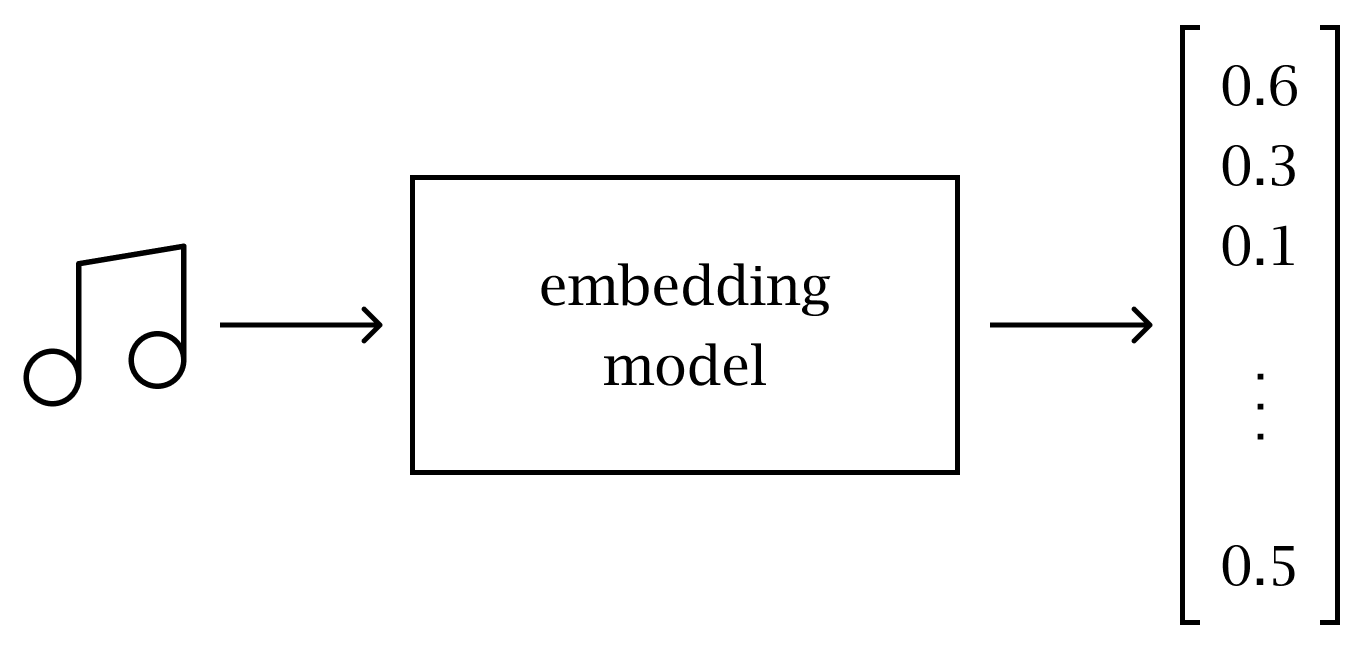
\includegraphics[width=\textwidth]{chapters/theory/data/figures/embedding.png}
        \caption{Unstructured data processed through a model to generate embeddings.}
        \label{fig:data-1-a}
    \end{subfigure}
    \hfill
    \begin{subfigure}[t]{0.48\textwidth}
        \centering
        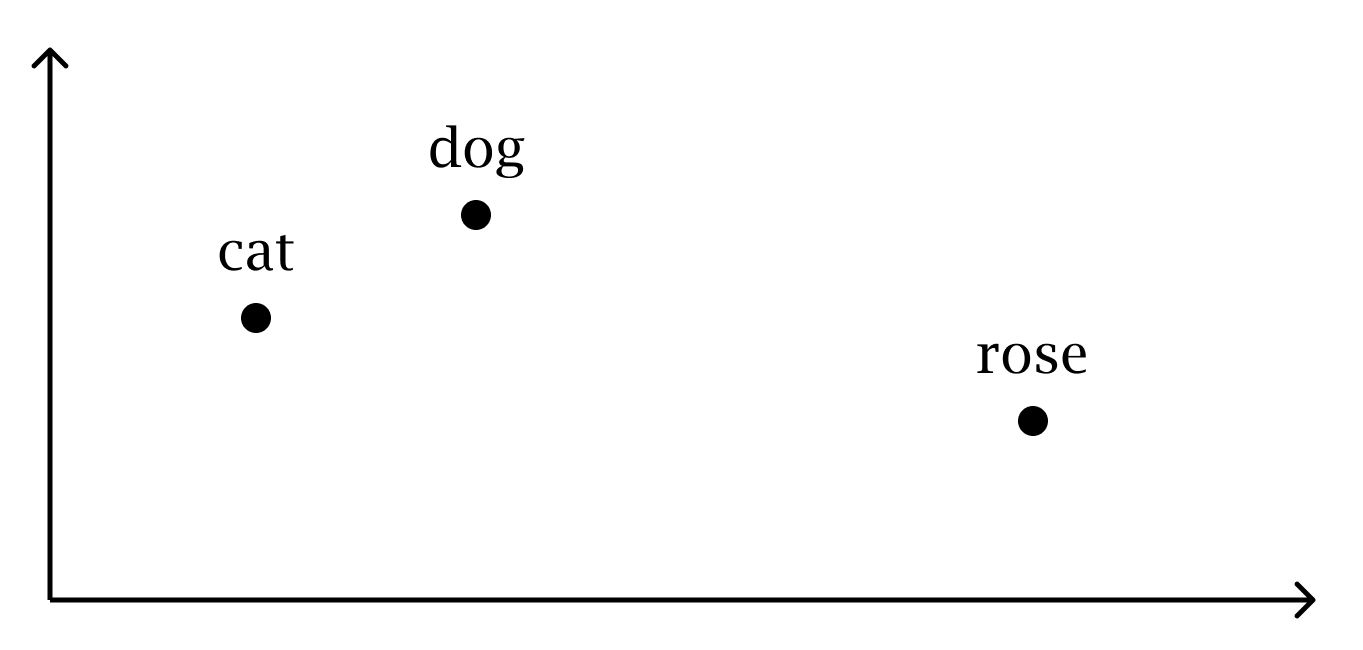
\includegraphics[width=\textwidth]{chapters/theory/data/figures/similarity.png}
        \caption{Semantically similar objects appear close together, while dissimilar ones are farther apart.}
        \label{fig:data-1-b}
    \end{subfigure}
    \caption{Illustration of the embedding process (a) and semantic similarity (b).}
    \label{fig:data-1}
\end{figure}

\begin{table}[h]
    \centering
    \renewcommand{\arraystretch}{2.3}
    \caption{Common similarity measures in vector databases.}
    \label{tab:distance-metrics}
    \begin{tabular}{|m{5cm}|m{8cm}|}
        \hline
        \textbf{Metric} & \textbf{Formula} \\ \hline
        $l_p$ (Minkowski) 
            & $\|x-y\|_p = \left(\sum_{i=1}^d |x_i-y_i|^p\right)^{1/p}$ \\ \hline
        $l_1$ (Manhattan) 
            & $\|x-y\|_1 = \sum_{i=1}^d |x_i-y_i|$ \\ \hline
        $l_2$ (Euclidean) 
            & $\|x-y\|_2 = \sqrt{\sum_{i=1}^d (x_i-y_i)^2}$ \\ \hline
        $l_\infty$ (Chebyshev) 
            & $\|x-y\|_\infty = \max_i |x_i-y_i|$ \\ \hline
        Cosine distance 
            & $d_{cos}(x,y) = 1 - (x \cdot y) / (\|x\|_2 \cdot \|y\|_2)
$ \\ \hline
        Dot (inner) product 
            & $s_{dot}(x,y) = \sum_{i=1}^d x_i \cdot y_i$ \\ \hline
        Hamming distance 
            & $d_{H}(x,y) = \sum_{i=1}^d 1(x_i \neq y_i)$ \\ \hline
    \end{tabular}
\end{table}
\section{Nearest Neighbor Search}

\subsection{Exact Nearest Neighbor Search}

\paragraph{Definition}

Given a set $P$ of points in a normed space $l_p^d$, preprocess $P$ so as to efficiently answer queries by returning a point $p \in P$ closest to a query point $q$.

This definition generalizes naturally to finding $k > 1$ nearest neighbors. In the $k$-NN search problem, $k$ points $p_1, \dots, p_k$ are returned such that each $p_i$ is the $i$-th closest point to $q$ \cite{Gionis-Indyk-Motwani-1999}.

\paragraph{Brute Force Approach}

The most straightforward approach for exact nearest neighbor search is the brute force (BF), or exhaustive search approach, which computes the distance between a query point and all points in the dataset to return the closest one. However, the computational cost of a single BF $k$-NN query using a chosen $l_p^d$ norm is $O(n \cdot d)$ \cite{Ukey-Yang-Li-Zhang-Hu-Zhang-2023}.

\paragraph{Structured Indexing Methods}

Several structured indexing methods have been proposed for exact $k$-NN search to efficiently handle low-dimensional datasets \cite{Ukey-Yang-Li-Zhang-Hu-Zhang-2023}:

\begin{itemize}
    \item \textbf{R-tree} and its variants (R*-tree, Hilbert R-tree, PR-tree): A height-balanced tree in which leaf nodes contain entries with an $n$-dimensional rectangle representing the bounding box of the associated spatial object, and non-leaf nodes contain entries that cover all rectangles in the entries of the lower node \cite{Guttman-1984}.
    \item \textbf{KD-tree}: A binary space-partitioning tree where each node stores a point from the dataset, and non-leaf nodes implicitly define a hyperplane that partitions the space into two child subtrees. At each level, the dimension with the largest spread is chosen, and the dataset is split at the median along that dimension \cite{Skrodzki-2019}.
    \item \textbf{Ball-tree}: A metric space-partitioning tree where each node defines a hypersphere containing a subset of the dataset. Each internal node is split in two steps: (1) the farthest point from the centroid of the points is selected as the first child centroid, and (2) the farthest point from this first centroid is selected as the second child centroid \cite{Dolatshah-Hadian-Minaei-2015}.
    \item \textbf{VP-tree} (and MVP-tree): A metric space-partitioning tree where each node selects a vantage point from its subset of points and partitions the points based on the median distance to this vantage point. Points closer than the median go to one child subtree, and points farther go to the other. This process is applied recursively, with distinct vantage points at each node, until leaf nodes containing a small number of points are reached \cite{Fu-Chan-Cheung-Moon-2000}.
\end{itemize}

\paragraph{Curse of Dimensionality}

As discussed above, these $k$-NN methods perform well in low-dimensional settings, but their efficiency degrades as the number of dimensions increases \cite{Ukey-Yang-Li-Zhang-Hu-Zhang-2023}.

The term \emph{curse of dimensionality} refers to the exponential growth of the volume of a space as the number of dimensions increases. This growth has significant implications for nearest neighbor search: as the dimensionality rises, data points become increasingly sparse. It causes distances between points to become increasingly similar, a phenomenon known as the \emph{concentration of measure}. As a result, the difference between the closest and farthest neighbors diminishes, reducing the effectiveness of standard distance metrics such as the $l_p^d$ norm.

Moreover, the impact of dimensionality depends on the relevance of the features: adding meaningful dimensions can improve contrast and preserve useful rankings of neighbors, while irrelevant dimensions reduce contrast and make distance-based queries less reliable \cite{Kouiroukidis-Evangelidis-2011}.

\subsection{Approximate Nearest Neighbor Search}

\paragraph{Definition}

Given a set $P$ of points in a normed space $l_p^d$, preprocess $P$ so as to efficiently answer queries by returning a point $p \in P$ for any given query point $q$, such that 
\[
d(p, q) \le (1 + \epsilon) \cdot d(q, P),
\]
where $d(q, P)$ is the distance from $q$ to its closest point in $P$.

This definition generalizes naturally to finding $k > 1$ approximate nearest neighbors. In the approximate $k$-NN search problem, $k$ points $p_1, \dots, p_k$ are returned such that the distance of $p_i$ to the query $q$ is at most $(1 + \epsilon)$ times the distance from the $i$-th nearest point to $q$ \cite{Gionis-Indyk-Motwani-1999}.

\paragraph{Motivation for Approximation}

In practical applications, the choice of features and distance metric is often heuristic, aiming to formalize what is fundamentally an intuitive notion of similarity. Consequently, insisting on exact nearest neighbors can be unnecessarily strict. Instead, determining an $\epsilon$-approximate nearest neighbor for a reasonable constant $\epsilon$ is usually sufficient for most purposes \cite{Indyk-Motwani-1998}.

Approximate nearest neighbor search aims to reduce the computational cost of similarity queries by relaxing the strict correctness requirement: the returned objects may not be the exact nearest neighbors. In practice, users often prefer faster responses that are sufficiently accurate rather than exact results, particularly in high-dimensional or large-scale datasets. The success of approximate methods relies on effectively balancing the trade-off between query efficiency and result quality \cite{Patella-Ciaccia-2009}.

\paragraph{Classification of Approximate Techniques}

Approximate nearest neighbor methods can be classified along several dimensions that reflect their applicability and design choices \cite{Patella-Ciaccia-2009}:

\begin{itemize}
    \item \textbf{Type of space} - Techniques can be specialized for different kinds of data spaces:
    \begin{itemize}
        \item Vector spaces with a specific $l_p^d$ distance.
        \item Vector spaces without restriction on the distance function.
        \item Metric spaces, where only the metric properties are assumed.
    \end{itemize}

    \item \textbf{Approximation mechanism} - How efficiency is achieved:
    \begin{itemize}
        \item Changing space: The search space is transformed or reduced (e.g., dimensionality reduction, bit approximations).
        \item Reducing comparisons: The search examines fewer candidates, either by
        \begin{itemize}
            \item aggressive pruning, or
            \item early stopping.
        \end{itemize}
    \end{itemize}

    \item \textbf{Quality guarantees} - Whether the method provides bounds on approximation errors:
    \begin{itemize}
        \item No guarantees: Heuristic approaches without formal bounds.
        \item Deterministic guarantees: Methods with provable maximum error bounds.
        \item Probabilistic guarantees: Techniques that guarantee correctness with a certain probability, either
        \begin{itemize}
            \item parametric, or
            \item non-parametric.
        \end{itemize}
    \end{itemize}

    \item \textbf{User interaction} - How parameters can be specified at query time:
    \begin{itemize}
        \item Static approach: Parameters are fixed at index construction; changing them requires rebuilding.
        \item Interactive approach: Users can adjust parameters dynamically at query time to trade off accuracy and efficiency.
    \end{itemize}
\end{itemize}

\begin{center}
    \vspace{0.5cm}
    *\hspace{2cm}*\hspace{2cm}*
    \vspace{0.3cm}
\end{center}

Unstructured data requires specialized representations to enable meaningful analysis. Embeddings map complex objects into a continuous vector space where semantic similarity can be quantified, while distance metrics determine how similarity is measured. Nearest neighbor search provides a framework for retrieving similar items, with exact methods offering precision and approximate methods trading some accuracy for efficiency. These concepts form the foundation for exploring specific algorithms for approximate nearest neighbor search, exemplified by hash-based, tree-based, and graph-based approaches.
    \chapter{Selected Algorithms}

\section{Locality-Sensitive Hashing (LSH)}

\subsection{Introduction to LSH}

Locality-Sensitive Hashing (LSH) is a hashing-based approach for approximate nearest neighbor (ANN) search. The concept of LSH was first introduced by Indyk and Motwani in 1998 \cite{Indyk-Motwani-1998} and later improved and generalized by Gionis, Indyk, and Motwani in 1999 \cite{Gionis-Indyk-Motwani-1999}.

The key idea of LSH is to design hash functions such that similar objects are mapped to the same bucket with high probability, while dissimilar objects are unlikely to collide. This property allows sublinear query time, as the search can be restricted to the elements stored in the buckets corresponding to the query point \cite{Gionis-Indyk-Motwani-1999}.

LSH significantly improved running time over previous methods for searching in high-dimensional spaces based on hierarchical tree decompositions \cite{Gionis-Indyk-Motwani-1999}. Although more recent graph-based and quantization-based methods, such as HNSW or IVF-PQ, often outperform LSH in practice, it remains a foundational algorithm with strong theoretical guarantees and continues to influence modern research in approximate nearest neighbor search.

\subsection{Description of LSH}

To simplify the presentation, the algorithm is described \cite{Gionis-Indyk-Motwani-1999} under two assumptions: (i) distances are measured with the $l_1$ norm, and (ii) all coordinates of the data points are positive integers. After these transformations, the minimum interpoint distance is guaranteed to be one.

Let $C$ be the largest coordinate value in all points in $P$. Each point 
$p = (x_{1}, \ldots, x_{d})$ is conceptually mapped to a binary vector in dimension $d' = C \cdot d$ by concatenating the unary representations of its coordinates:
\[
v(p) = \text{Unary}_{C}(x_{1}) \;\Vert\; \dots \Vert\; \text{Unary}_{C}(x_{d}),
\]
where $\text{Unary}_{C}(x)$ is a binary string of $x$ ones followed by $C - x$ zeros. This mapping preserves distances: the $l_1$ distance in the original space equals the $d_H$ distance in the Hamming space $H^{d'}$. In practice, the unary expansion is not materialized explicitly; it is used only as a conceptual framework for defining the algorithms.

\newpage

\paragraph{Hash Functions}

The LSH scheme uses $l$ different hash tables, each associated with its own hash function $g_{j}$, for $j = 1, \dots, l$. For each hash table, the function $g_{j}$ is defined by selecting $k$ coordinates uniformly at random (with replacement) from $\{1, \dots, d'\}$ and projecting the binary vector $v(p)$ onto these positions, producing $g_{j}(p)$. The parameter $k$ is chosen to maximize the probability that a point close to a query $q$ falls into the same bucket as $q$, while minimizing the probability that a distant point collides in the same bucket. Each point $p \in P$ is then stored in the corresponding bucket $g_{j}(p)$ across all $l$ tables (Figure~\ref{fig:lsh-1}).

Since the number of buckets can be very large, a second level of hashing is used to compress them into a hash table of fixed size $M$, with each bucket limited to a maximum capacity of $B$ \cite{Gionis-Indyk-Motwani-1999}. The selection of the parameters $l$ and $k$ is discussed in the next section.

\begin{figure}[H]
    \centering
    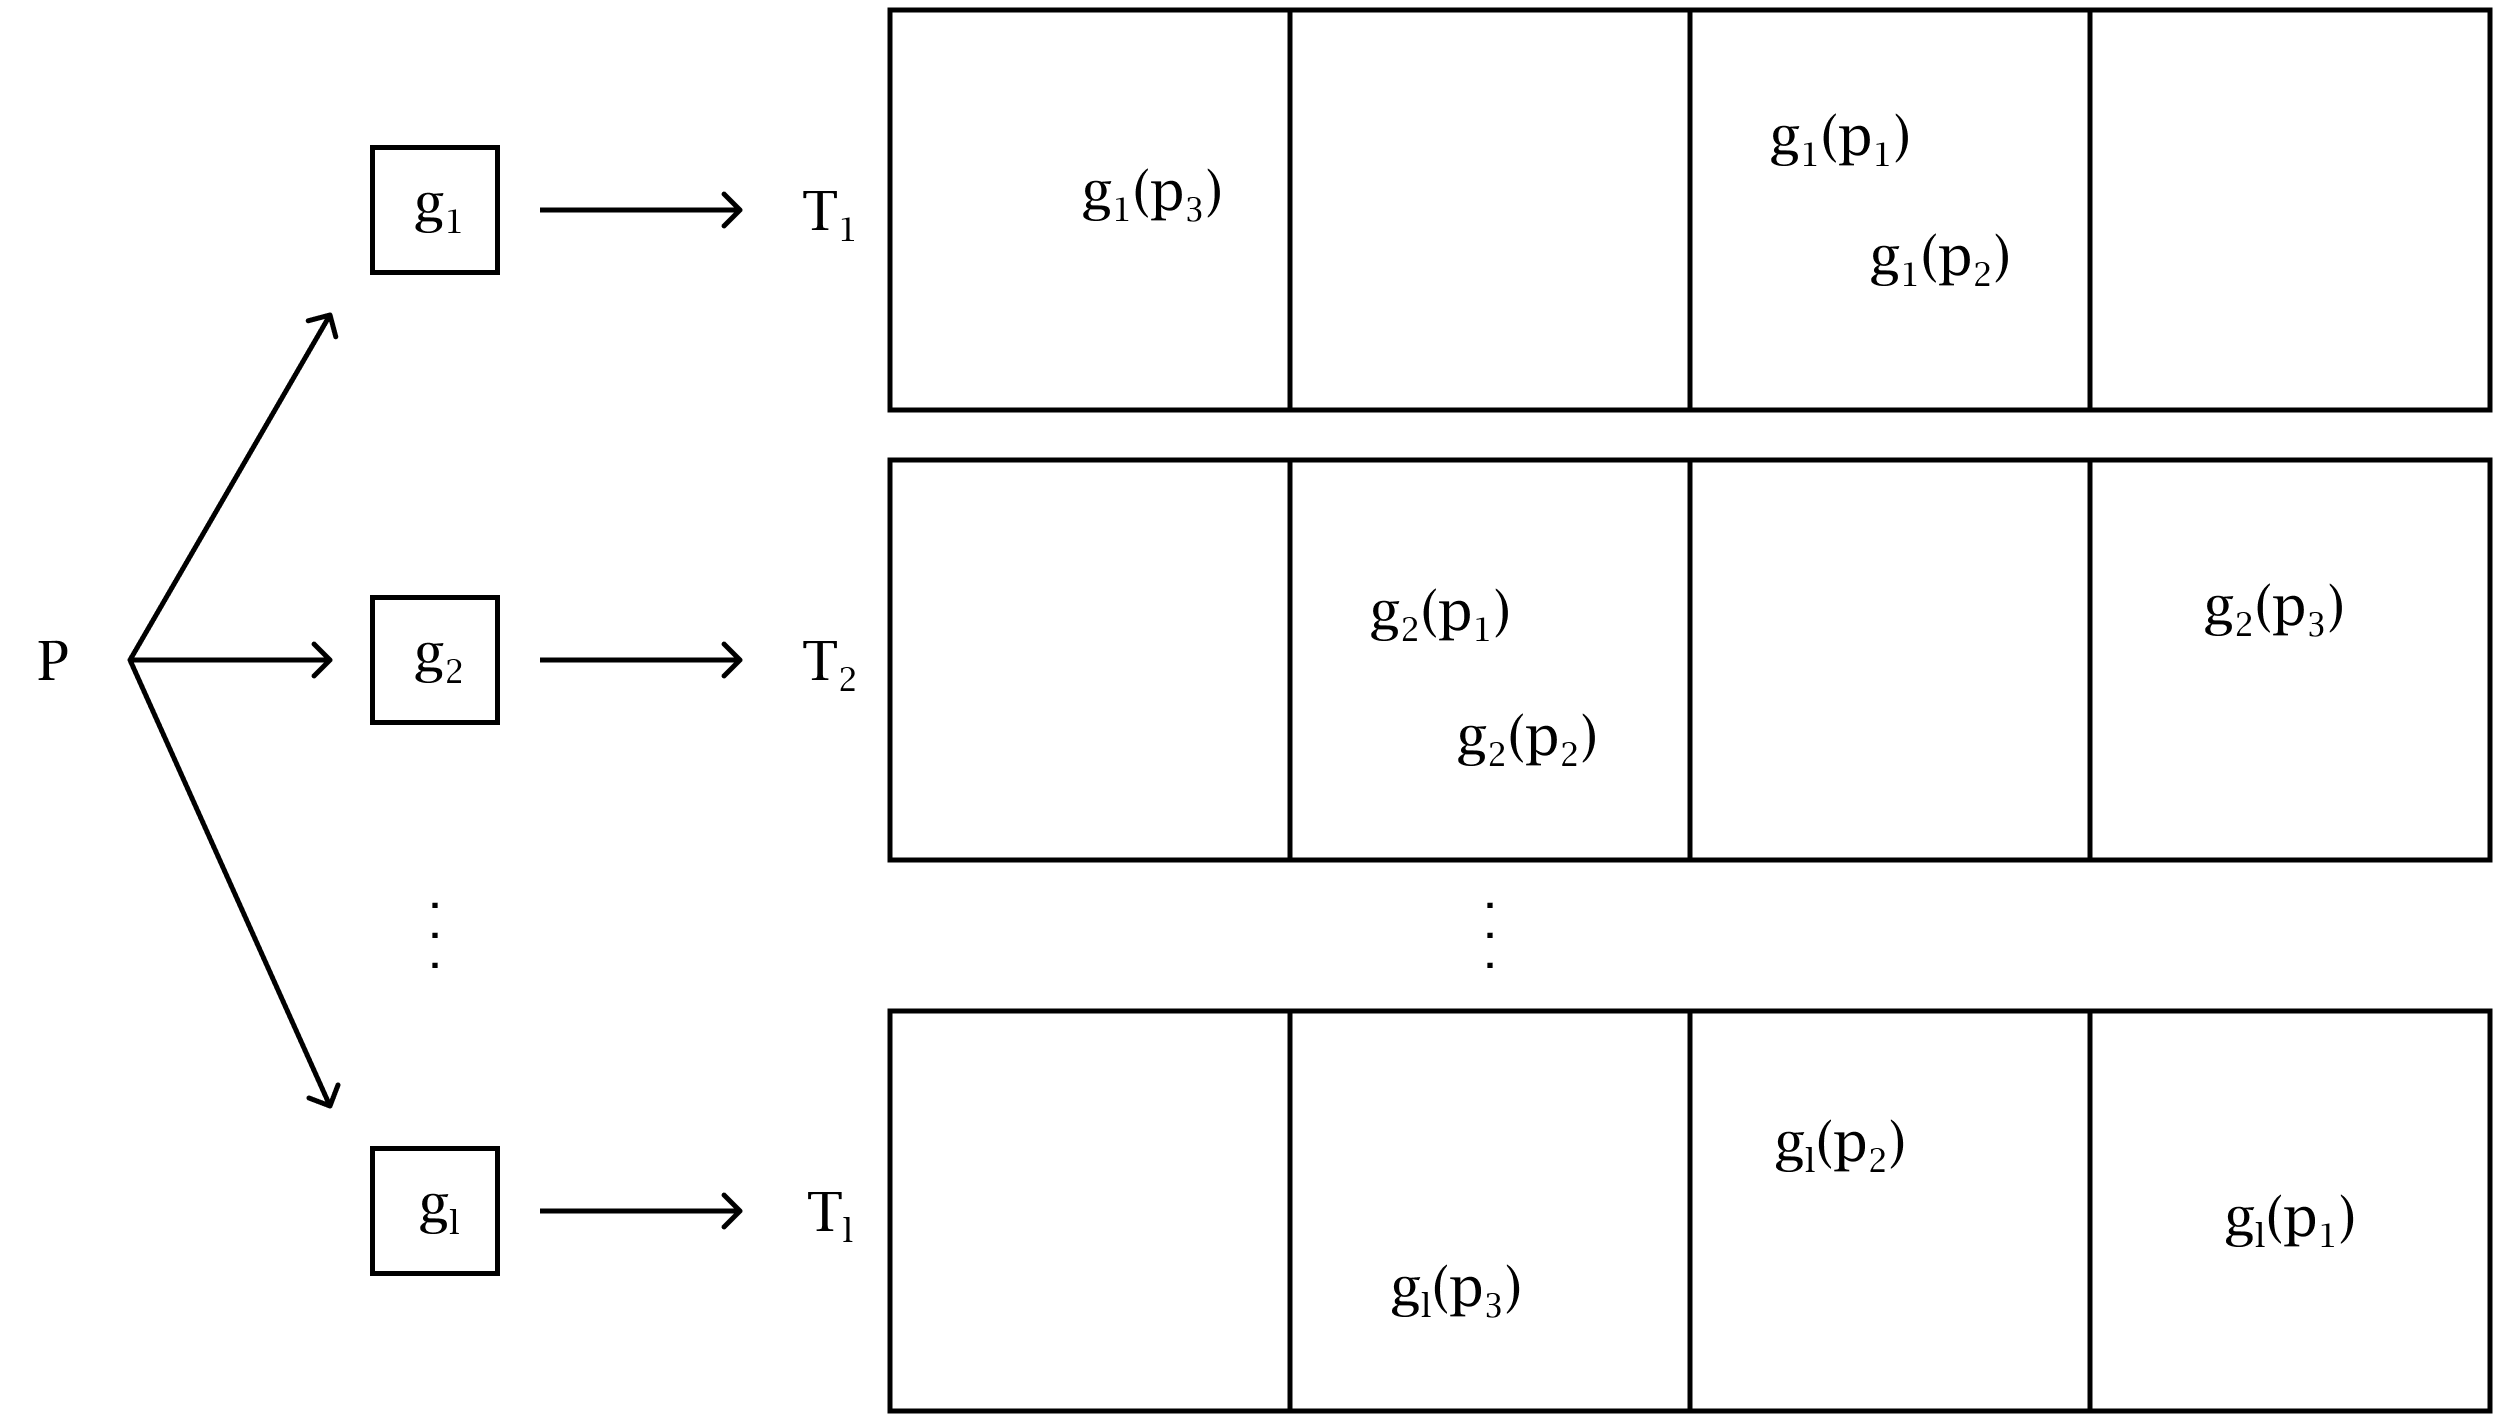
\includegraphics[width=0.9\textwidth]{chapters/algorithms/lsh/figures/hashing.png}
    \caption{LSH hashing process. Each data point $p \in P$ is projected via hash functions $g_j$ into buckets across $l$ hash tables.}
    \label{fig:lsh-1}
\end{figure}

\subsubsection{Indexing}

The indexing stage (Algorithm~\ref{alg:lsh-1}) constructs the $l$ hash tables and distributes the dataset points into the appropriate buckets:

\begin{algorithm}[H]
    \caption{BUILD-INDEX \cite{Gionis-Indyk-Motwani-1999}}
    \label{alg:lsh-1}
    \begin{algorithmic}[1]
        \Require points $P$, number of hash tables $l$
        \Ensure hash tables $T$
    
        \For{$i \gets 1 \dots l$}
            \State generate random hash function $g_i(\cdot)$ and initialize hash table $T_i$
            
            \For{each $p \in P$}
                \State store point $p$ in bucket $g_i(p)$ of hash table $T_i$
            \EndFor
        \EndFor
    \end{algorithmic}
\end{algorithm}

\subsubsection{Querying}

To answer a query, the algorithm (Algorithm~\ref{alg:lsh-2}) hashes the query point $q$ into each of the $l$ tables, retrieves candidate points from the corresponding buckets, and returns the $k$ nearest neighbors from the candidate set:

\begin{algorithm}[H]
    \caption{K-NN-SEARCH \cite{Gionis-Indyk-Motwani-1999}}
    \label{alg:lsh-2}
    \begin{algorithmic}[1]
        \Require $l$ hash tables $T$, query point $q$, number of nearest neighbors $k$
        \Ensure up to $k$ approximate nearest neighbors of $q$
        
        \State $S \gets \emptyset$ \Comment{candidate set}
        
        \For{$i \gets 1 \dots l$}
            \State $S \gets S \cup \{$points in bucket $g_i(q)$ of hash table $T_i\}$
        \EndFor
        
        \State \Return up to $k$ nearest neighbors of $q$ in $S$
    \end{algorithmic}
\end{algorithm}

\subsection{Analysis of LSH}

The main intuition behind LSH is that the probability of two points colliding in the same hash bucket decreases as the distance between them increases, which is formalized as follows \cite{Gionis-Indyk-Motwani-1999}. Let $D(\cdot, \cdot)$ be a distance function on a set $S$, and for any $p \in S$ let $\mathcal{B}(p, r)$ denote the set of elements from $S$ within distance $r$ from $p$. A family $\mathcal{H} = \{h: S \to U\}$ is called $(r_1, r_2, p_1, p_2)$-sensitive for $D(\cdot, \cdot)$ if for any $p, q \in S$:

\begin{itemize}
    \item If $p \in \mathcal{B}(q, r_1)$, then $\Pr_{\mathcal{H}}[h(q) = h(p)] \ge p_1$.
    \item If $p \notin \mathcal{B}(q, r_2)$, then $\Pr_{\mathcal{H}}[h(q) = h(p)] \le p_2$.
\end{itemize}

For a locality-sensitive family to be useful, it must hold that $p_1 > p_2$ and $r_1 < r_2$. This ensures that points close to the query are likely to collide in a hash bucket, while distant points are unlikely to.

\paragraph{Hamming Locality-Sensitive Family}

When the distance function is the Hamming distance, the family of projections on one coordinate is locality-sensitive. Specifically, let $S = H^{d'}$ and $D(p, q) = d_H(p, q)$ for $p, q \in H^{d'}$. Then for any $r, \epsilon > 0$, the family
\[
\mathcal{H}_{d'} = \Bigl\{ h_i : h_i\Bigl((b_1, \dots, b_{d'})\Bigr) = b_i, \; i = 1, \dots, d' \Bigr\}
\]
is 
\[
\Big(r, r(1 + \epsilon), 1 - \frac{r}{d'}, 1 - \frac{r(1 + \epsilon)}{d'}\Big)\text{-sensitive}.
\] 
That is, points within distance $r$ collide with probability at least $1 - r/d'$, while points farther than $r(1 + \epsilon)$ collide with probability at most $1 - r(1 + \epsilon)/d'$ \cite{Gionis-Indyk-Motwani-1999}.

\paragraph{Arbitrary Locality-Sensitive Family}

The algorithm can be generalized to any locality-sensitive family $\mathcal{H}$. In this case, each hash function is defined as
\[
g_i(p) = (h_{i_1}(p), \dots, h_{i_k}(p)),
\]  
where $h_{i_1}, \dots, h_{i_k}$ are randomly chosen from $\mathcal{H}$ with replacement. As before, $l$ such functions $g_1, \dots, g_l$ are constructed to build $l$ hash tables \cite{Gionis-Indyk-Motwani-1999}.

\paragraph{Correctness via the $(r, \epsilon)$-Neighbor Problem}

Formally, the algorithm is shown \cite{Gionis-Indyk-Motwani-1999} to correctly solve the so-called $(r, \epsilon)$-Neighbor problem, which asks whether there exists a point $p$ within a fixed distance $r_1 = r$ of the query $q$, or whether all points are at least distance $r_2 = (1 + \epsilon)r$ away. In particular, the LSH algorithm solves this problem for a proper choice of parameters $k$ and $l$, depending on $r$ and $\epsilon$. More precisely, for the set of points $P' \subseteq P$ farther than $r_2$ from $q$, the algorithm correctly solves the $(r, \epsilon)$-Neighbor problem if the following two properties hold:

\begin{itemize}
    \item[\textbf{P1}] If there exists a point within distance $r_1$ of the query, then at least one of the hash functions $g_1, \dots, g_l$ maps it to the same bucket as the query.
    \item[\textbf{P2}] The total number of hash buckets pointed to by the query that contain only points from $P'$ is bounded by $c \cdot l$, for some constant $c$.
\end{itemize}

Intuitively, P1 ensures that close points are likely to be retrieved by the query, while P2 guarantees that the number of far points incorrectly considered is limited, keeping the search efficient. As proven in \cite{Gionis-Indyk-Motwani-1999}, by choosing the parameters:

\[
k = \log_{\frac{1}{p_2}} \frac{n}{B}, \quad 
l = \left( \frac{n}{B} \right)^\rho, \quad 
\rho = \frac{\ln \frac{1}{p_1}}{\ln \frac{1}{p_2}}
\]

both properties P1 and P2 hold with probability at least $1/2 - 1/e \ge 0.132$, ensuring the correctness of the LSH algorithm.\newline

When instantiated for the Hamming locality-sensitive family, it can be shown that
\[
\rho \le \frac{1}{1 + \epsilon}
\]
under the assumption that $r < d'/\ln n$ which can be easily satisfied. Thus, the expected query time of the LSH algorithm is sublinear in the number of points $n$. Specifically, for a dataset of $n$ points in dimension $d$, the query time is $O\bigl(d \cdot n^{1 / (1 + \epsilon)}\bigr)$ \cite{Gionis-Indyk-Motwani-1999}.

\paragraph{Connection to the $\epsilon$-NNS Problem}

While the $(r, \epsilon)$-Neighbor problem is central for the theoretical analysis of LSH, in practice the main objective is to solve the $\epsilon$-Nearest Neighbor Search ($\epsilon$-NNS) problem. This problem can be reduced to a sequence of $(r, \epsilon)$-Neighbor instances for different values of $r$, specifically $r_0, r_0(1 + \epsilon), r_0(1 + \epsilon)^2, \dots, r_{\max}$, where $r_0$ and $r_{\max}$ denote the smallest and the largest possible distance between the query and the dataset, respectively \cite{Gionis-Indyk-Motwani-1999}. By testing successive $(r, \epsilon)$-Neighbor instances for increasing values of $r$, one can identify the smallest radius at which a neighbor is detected.

However, empirical evidence suggests that in most cases a single fixed value of $r$ is sufficient, since the distribution of distances between queries and the dataset typically depends more on the intrinsic properties of the data than on the particular query point. Consequently, in practice a fixed choice of $r$ is often adopted, which also fixes the values of $k$ and $l$ for the entire dataset \cite{Gionis-Indyk-Motwani-1999}.
\section{Approximate Nearest Neighbors Oh Yeah (Annoy)}

\subsection{Introduction to Annoy}

Approximate Nearest Neighbors Oh Yeah (Annoy) is a tree-based approach for approximate nearest neighbor (ANN) search. It was developed by Bernhardsson during Spotify's Hack Week in 2013 \cite{spotify-annoy} for music recommendation.

An Annoy tree is constructed using random projections: at each intermediate node, a hyperplane is defined by sampling two points from the subset and placing it equidistant from them, thereby dividing the space into two subspaces. The recursive process continues until a single tree is formed \cite{spotify-annoy}.

Although Annoy does not provide formal theoretical guarantees like LSH or HNSW, it has demonstrated good empirical performance. By offering a favorable trade-off between query speed, memory usage, and accuracy \cite{Li-Zhang-Sun-Wang-Zhang-Lin-2016}, it is often used in practice and is also referenced in research on approximate nearest neighbor search.

The Annoy implementation is available at GitHub\footnote{\url{https://github.com/spotify/annoy}}.

\subsection{Description of Annoy}

The description provided in this section is based on the official Spotify Annoy repository \cite{spotify-annoy} and Bernhardsson's presentation on Annoy \cite{erikbern-ann-presentation}.

\subsubsection{Indexing: Tree}

\noindent
To illustrate the construction of an Annoy index, a set of points representing vectors in the space is shown (Figure~\ref{fig:annoy-1}). For visualization purposes, a 2-dimensional example is used; in practice, vectors typically reside in much higher-dimensional spaces.

\begin{figure}[H]
    \centering
    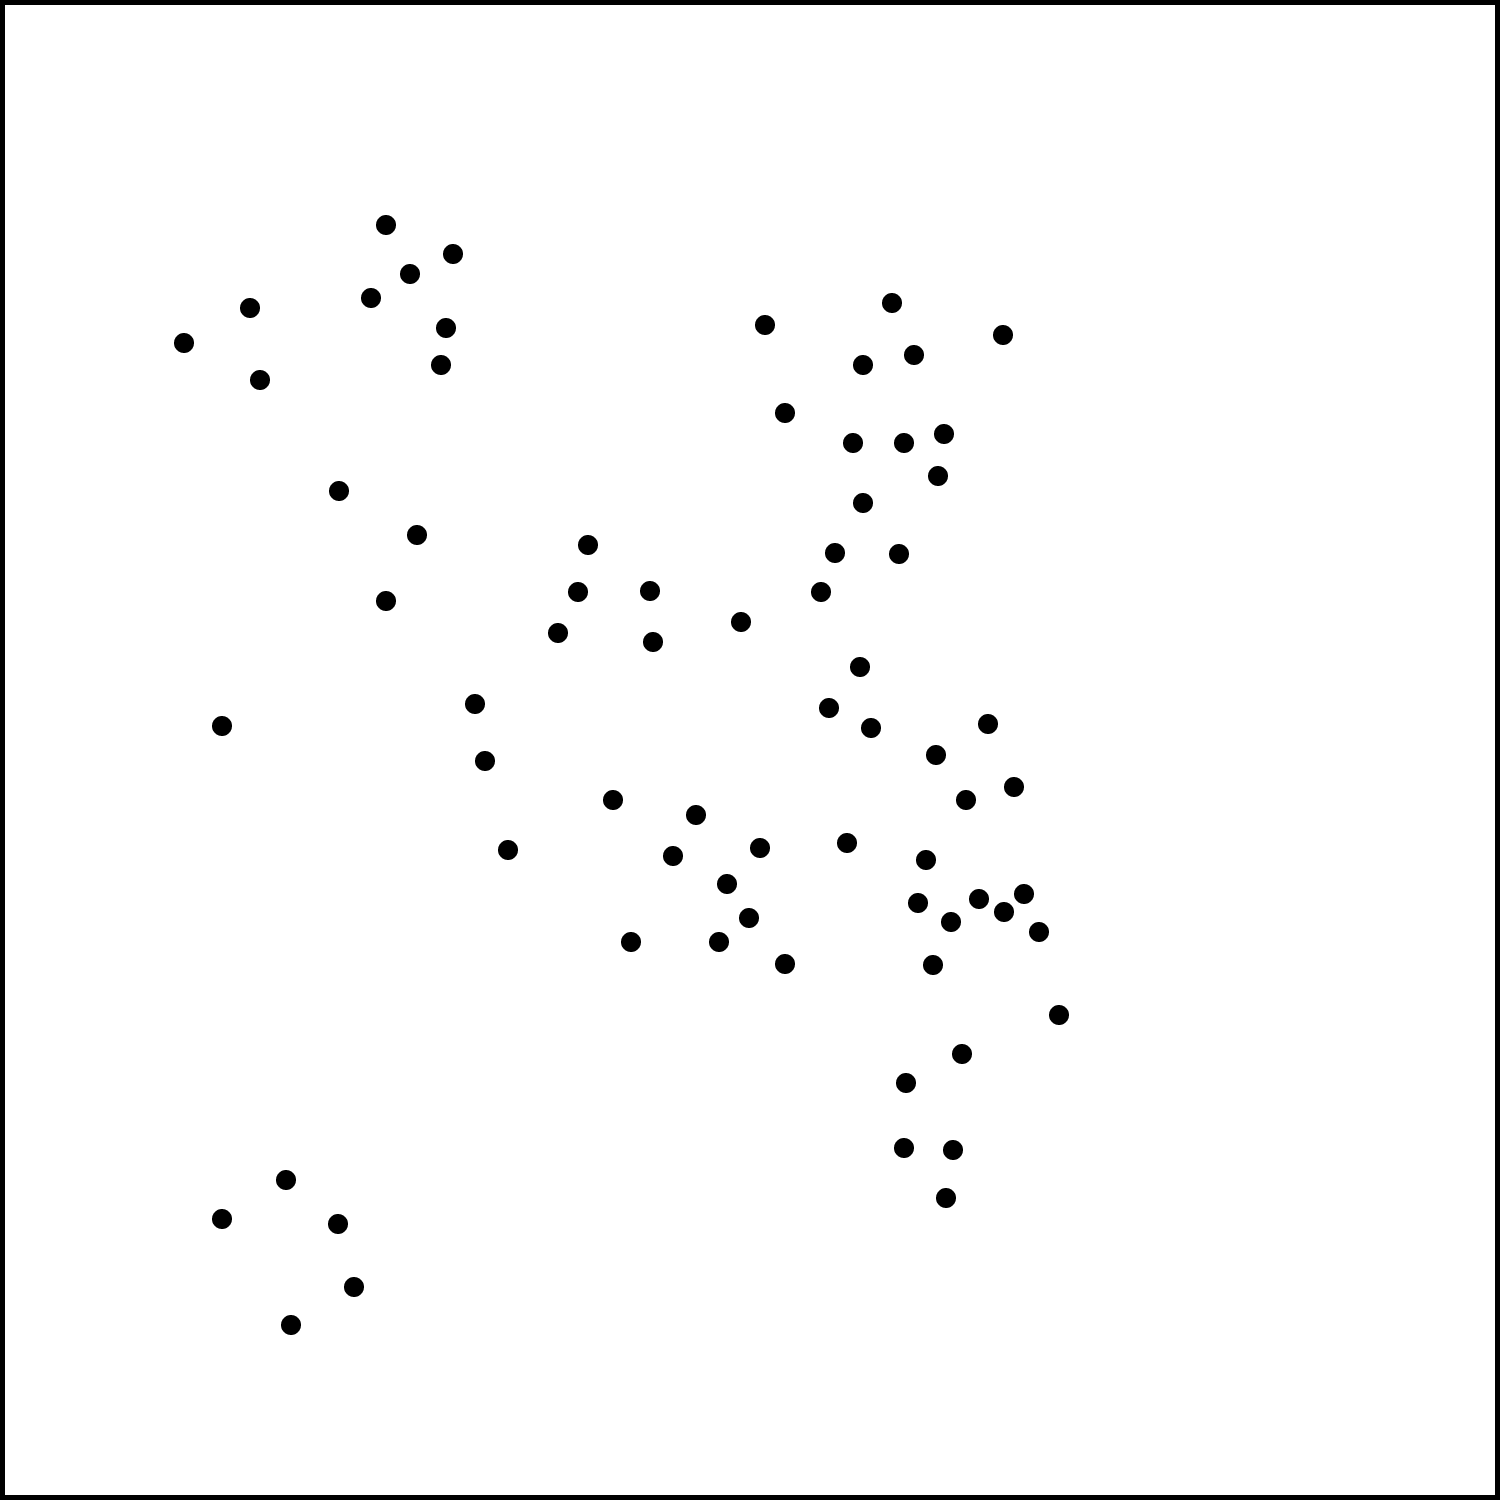
\includegraphics[width=0.48\textwidth]{chapters/algorithms/annoy/figures/points.png}
    \caption{Initial set of points in 2D space.}
    \label{fig:annoy-1}
\end{figure}

\newpage

\noindent
The goal is to construct a data structure that allows nearest neighbor queries to be answered in sublinear time. To support this, Annoy builds a binary tree in which each node represents a random partition of the space. The process begins with a single split of the space (Figure~\ref{fig:annoy-2-a}).

Each split is performed by randomly selecting two points and constructing a hyperplane equidistant from them. This hyperplane divides the current subspace into two halves, with each half assigned to a child node in the binary tree. The partitioning continues recursively for each resulting subspace (Figure~\ref{fig:annoy-2-b}). In practice, the hyperplane itself does not need to be explicitly computed; each vector is assigned to a side based on which of the two selected points it is closer to.

\begin{figure}[H]
    \centering
    \begin{subfigure}[t]{0.48\textwidth}
        \centering
        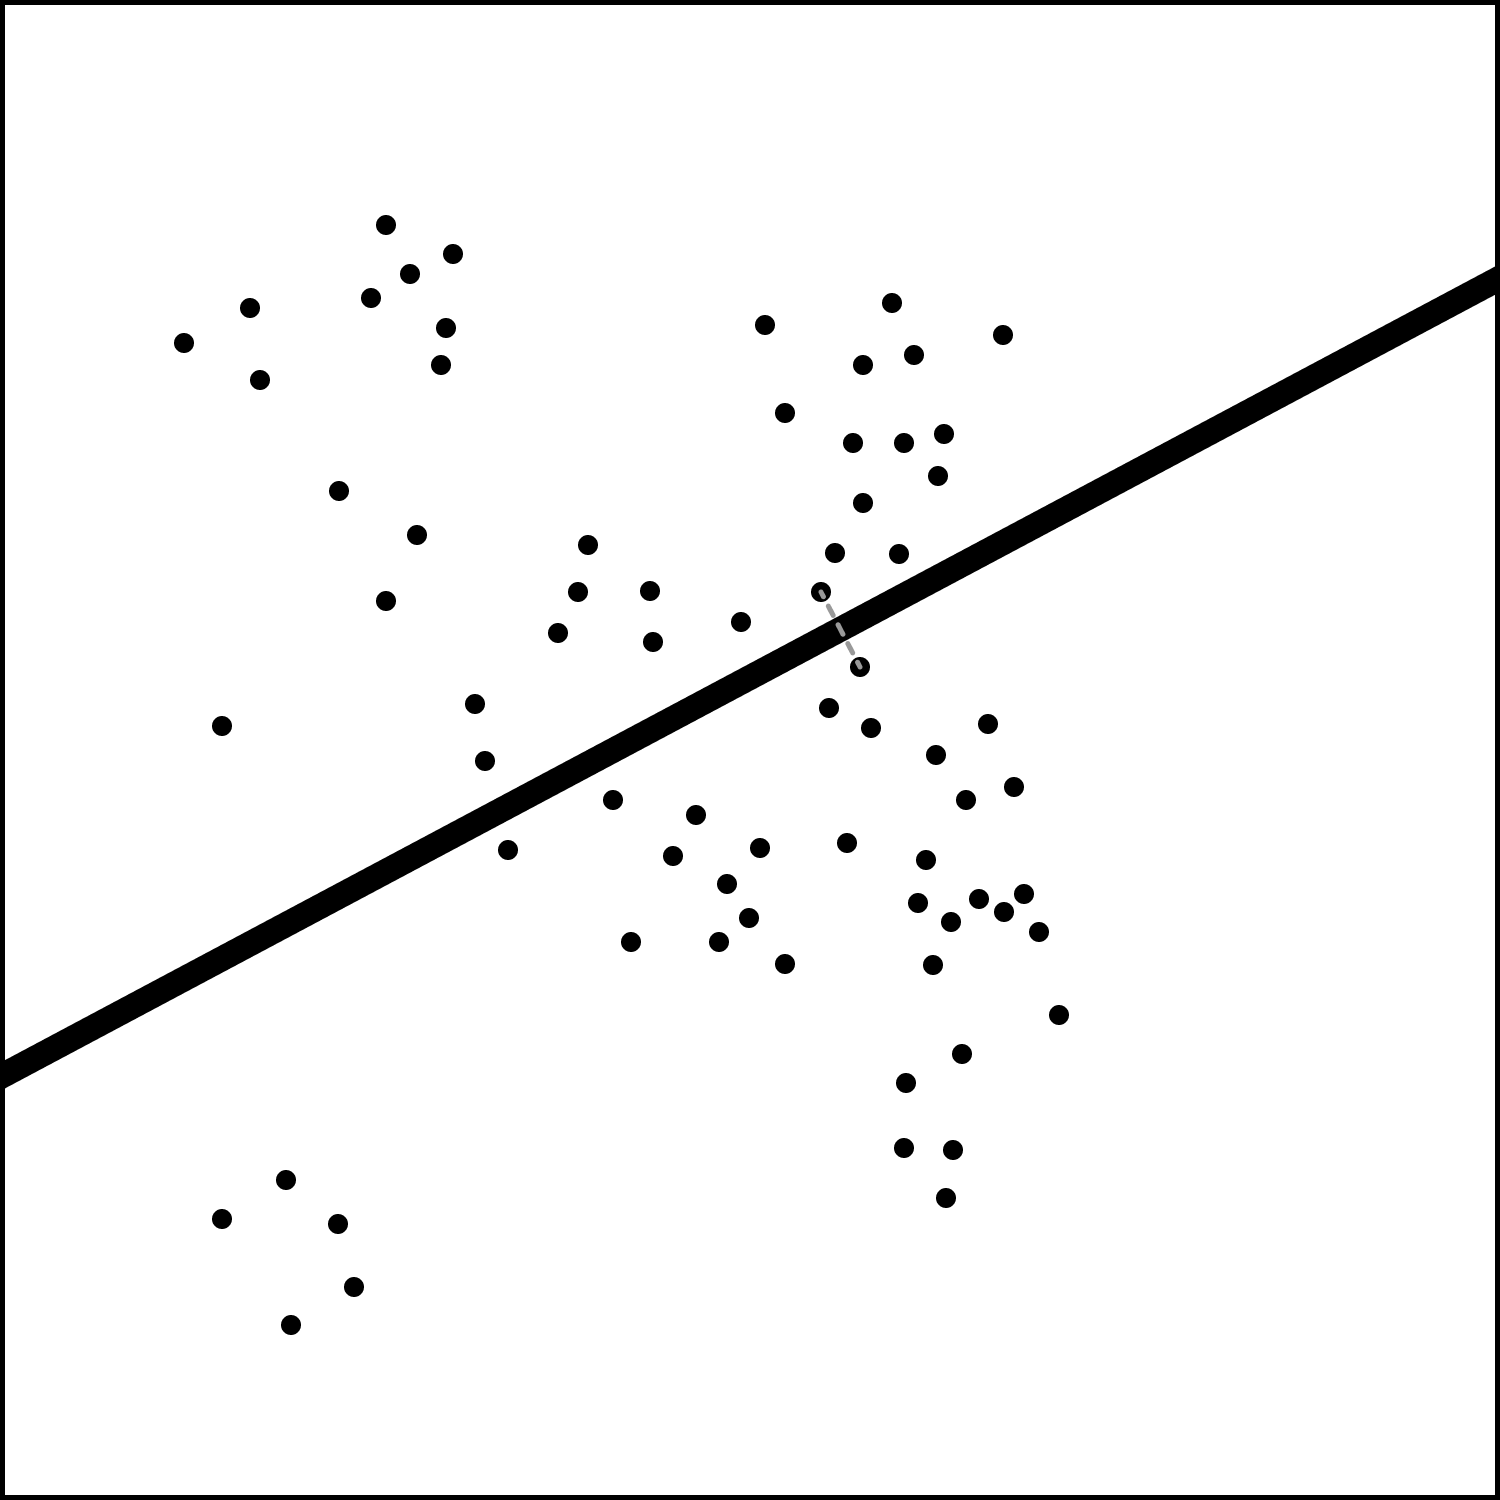
\includegraphics[width=\textwidth]{chapters/algorithms/annoy/figures/initial-split.png}
        \caption{Initial split of the space using a hyperplane.}
        \label{fig:annoy-2-a}
    \end{subfigure}
    \hfill
    \begin{subfigure}[t]{0.48\textwidth}
        \centering
        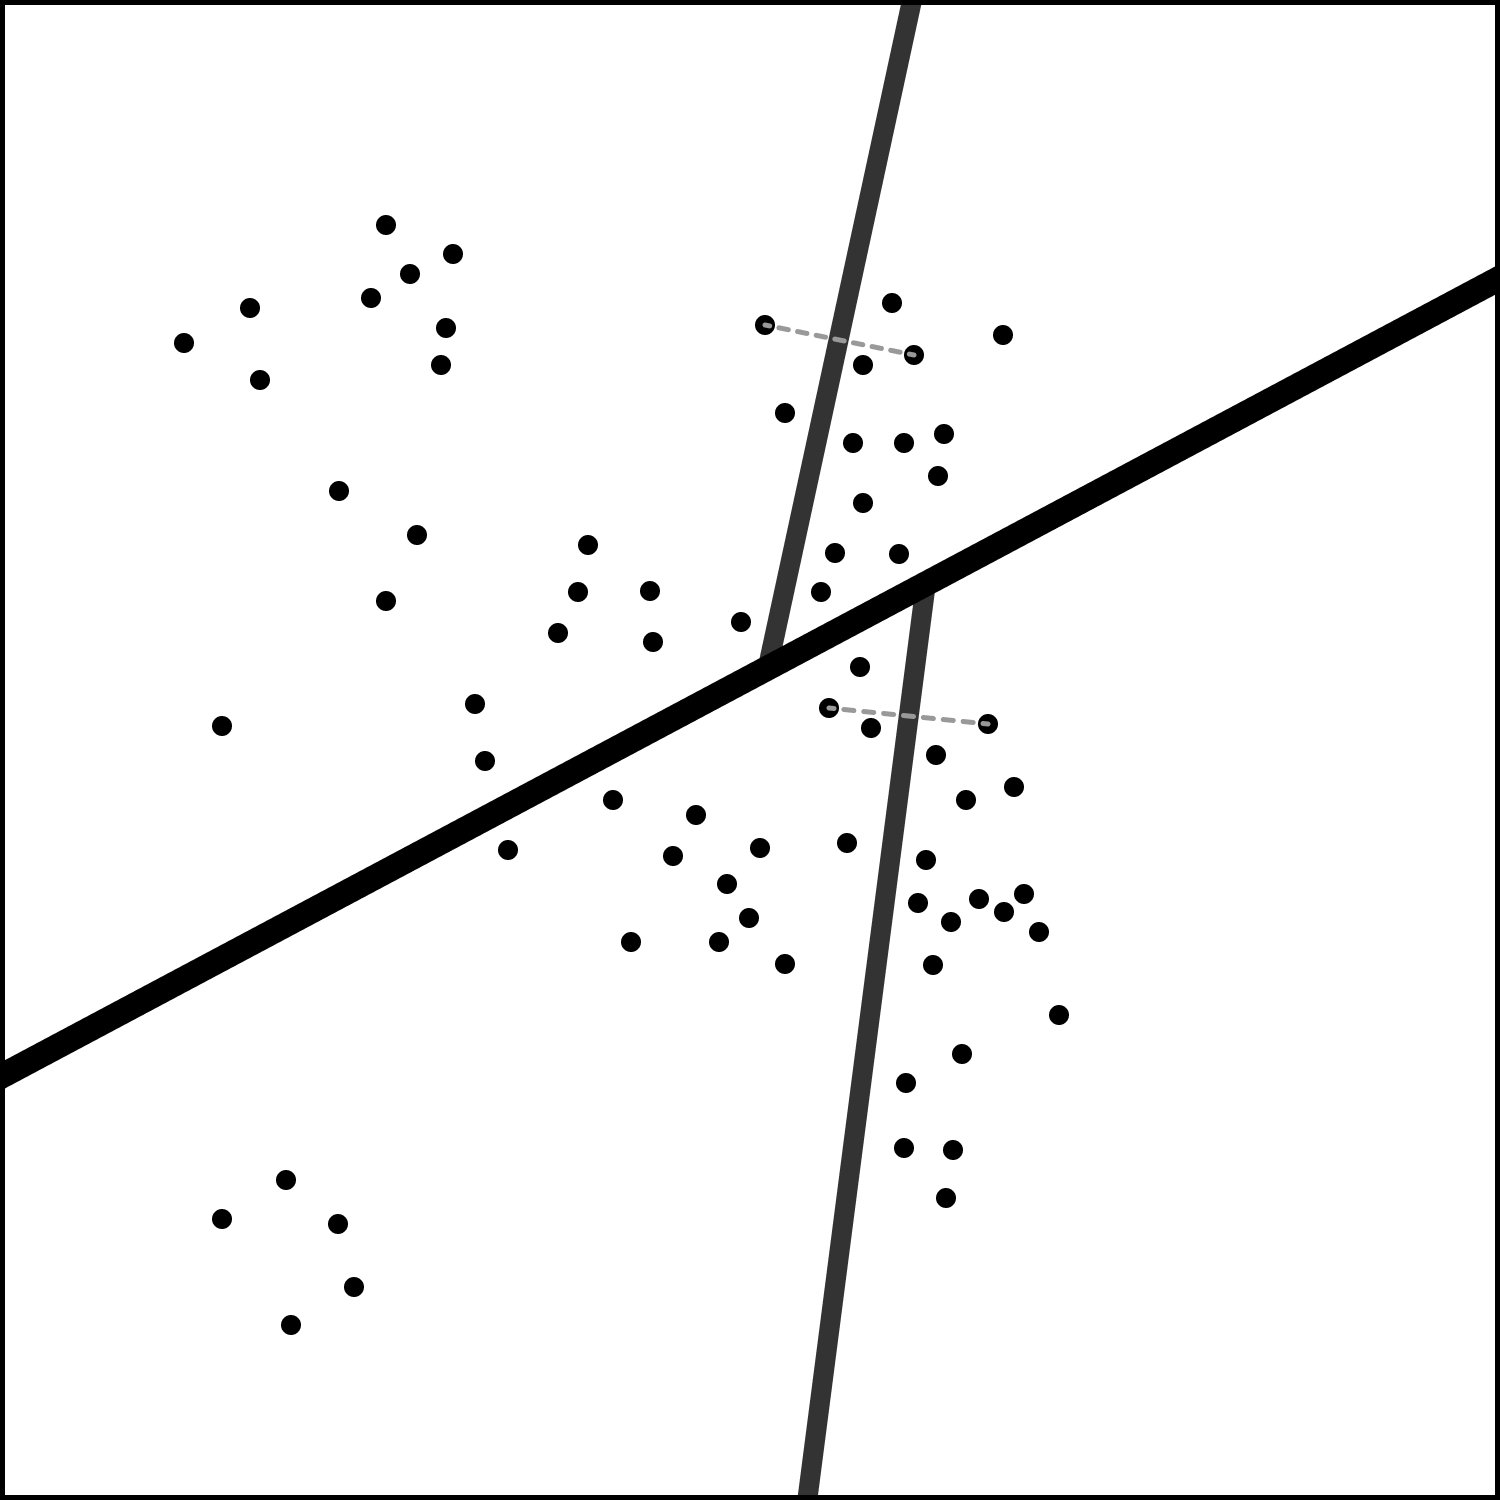
\includegraphics[width=\textwidth]{chapters/algorithms/annoy/figures/recursive-splits.png}
        \caption{Recursive splits of subspaces.}
        \label{fig:annoy-2-b}
    \end{subfigure}
    \caption{Initial and recursive splits in the construction of an Annoy tree.}
    \label{fig:annoy-2}
\end{figure}

\noindent
The recursive partitioning proceeds until each leaf node contains at most $K$ points (Figure~\ref{fig:annoy-3}).

\begin{figure}[H]
    \centering
    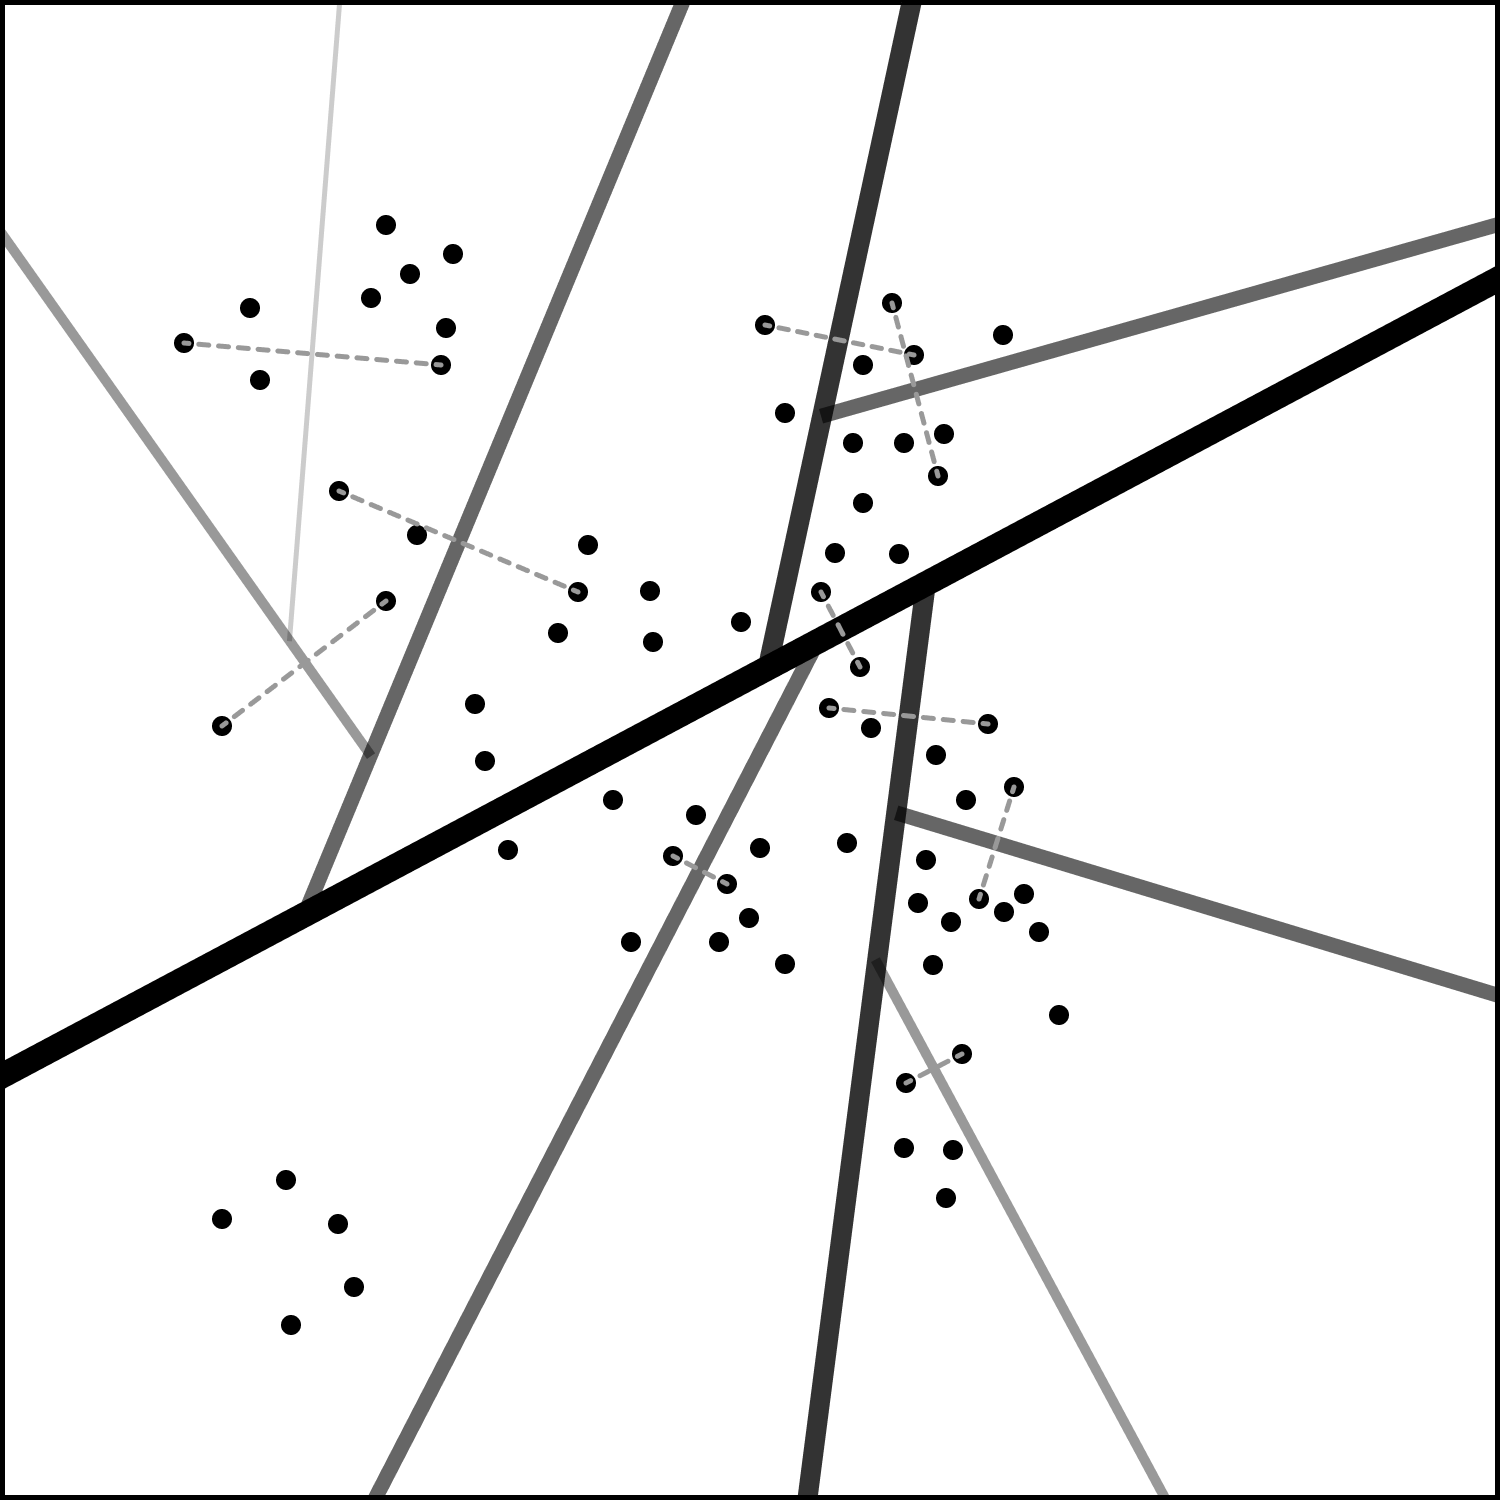
\includegraphics[width=0.48\textwidth]{chapters/algorithms/annoy/figures/final-splits.png}
    \caption{Final partitions of the space with a maximum of $K = 10$ points per leaf.}
    \label{fig:annoy-3}
\end{figure}

\noindent
The structure of the binary tree (Figure~\ref{fig:annoy-4}) reflects the hierarchical partitioning of the space. Each leaf node in the tree corresponds to one of the final subspaces.

\begin{figure}[H]
    \centering
    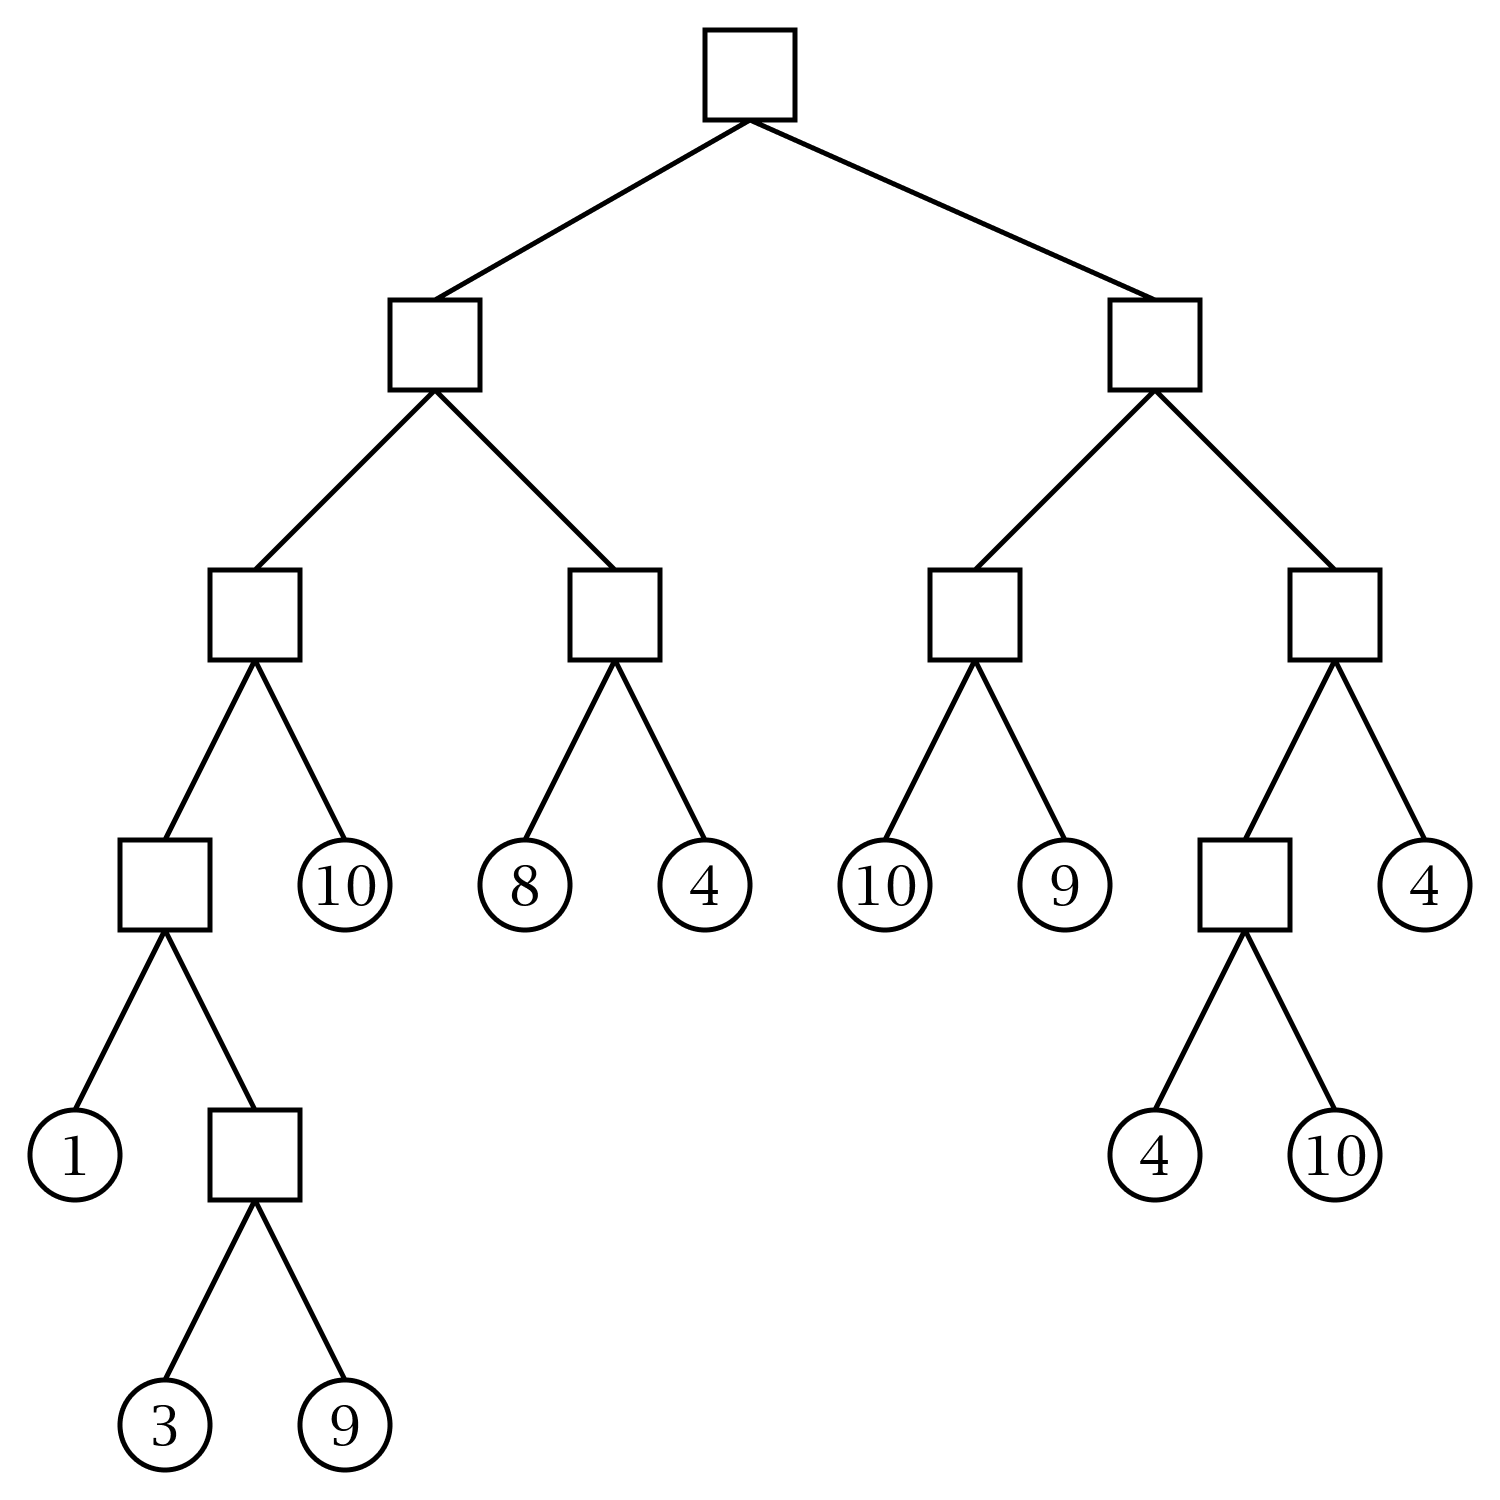
\includegraphics[width=0.48\textwidth]{chapters/algorithms/annoy/figures/tree-1.png}
    \caption{Binary tree corresponding to the final partitioning of the space.}
    \label{fig:annoy-4}
\end{figure}

\noindent
Points that are close to each other are likely to remain within the same or neighboring leaf nodes. Consequently, hyperplanes rarely separate points that are near each other, preserving local proximity within the tree structure.

\subsubsection{Querying}

\noindent
Once the space has been partitioned, a query point is evaluated within the structure to search for its nearest neighbors (Figure~\ref{fig:annoy-5}).

\begin{figure}[H]
    \centering
    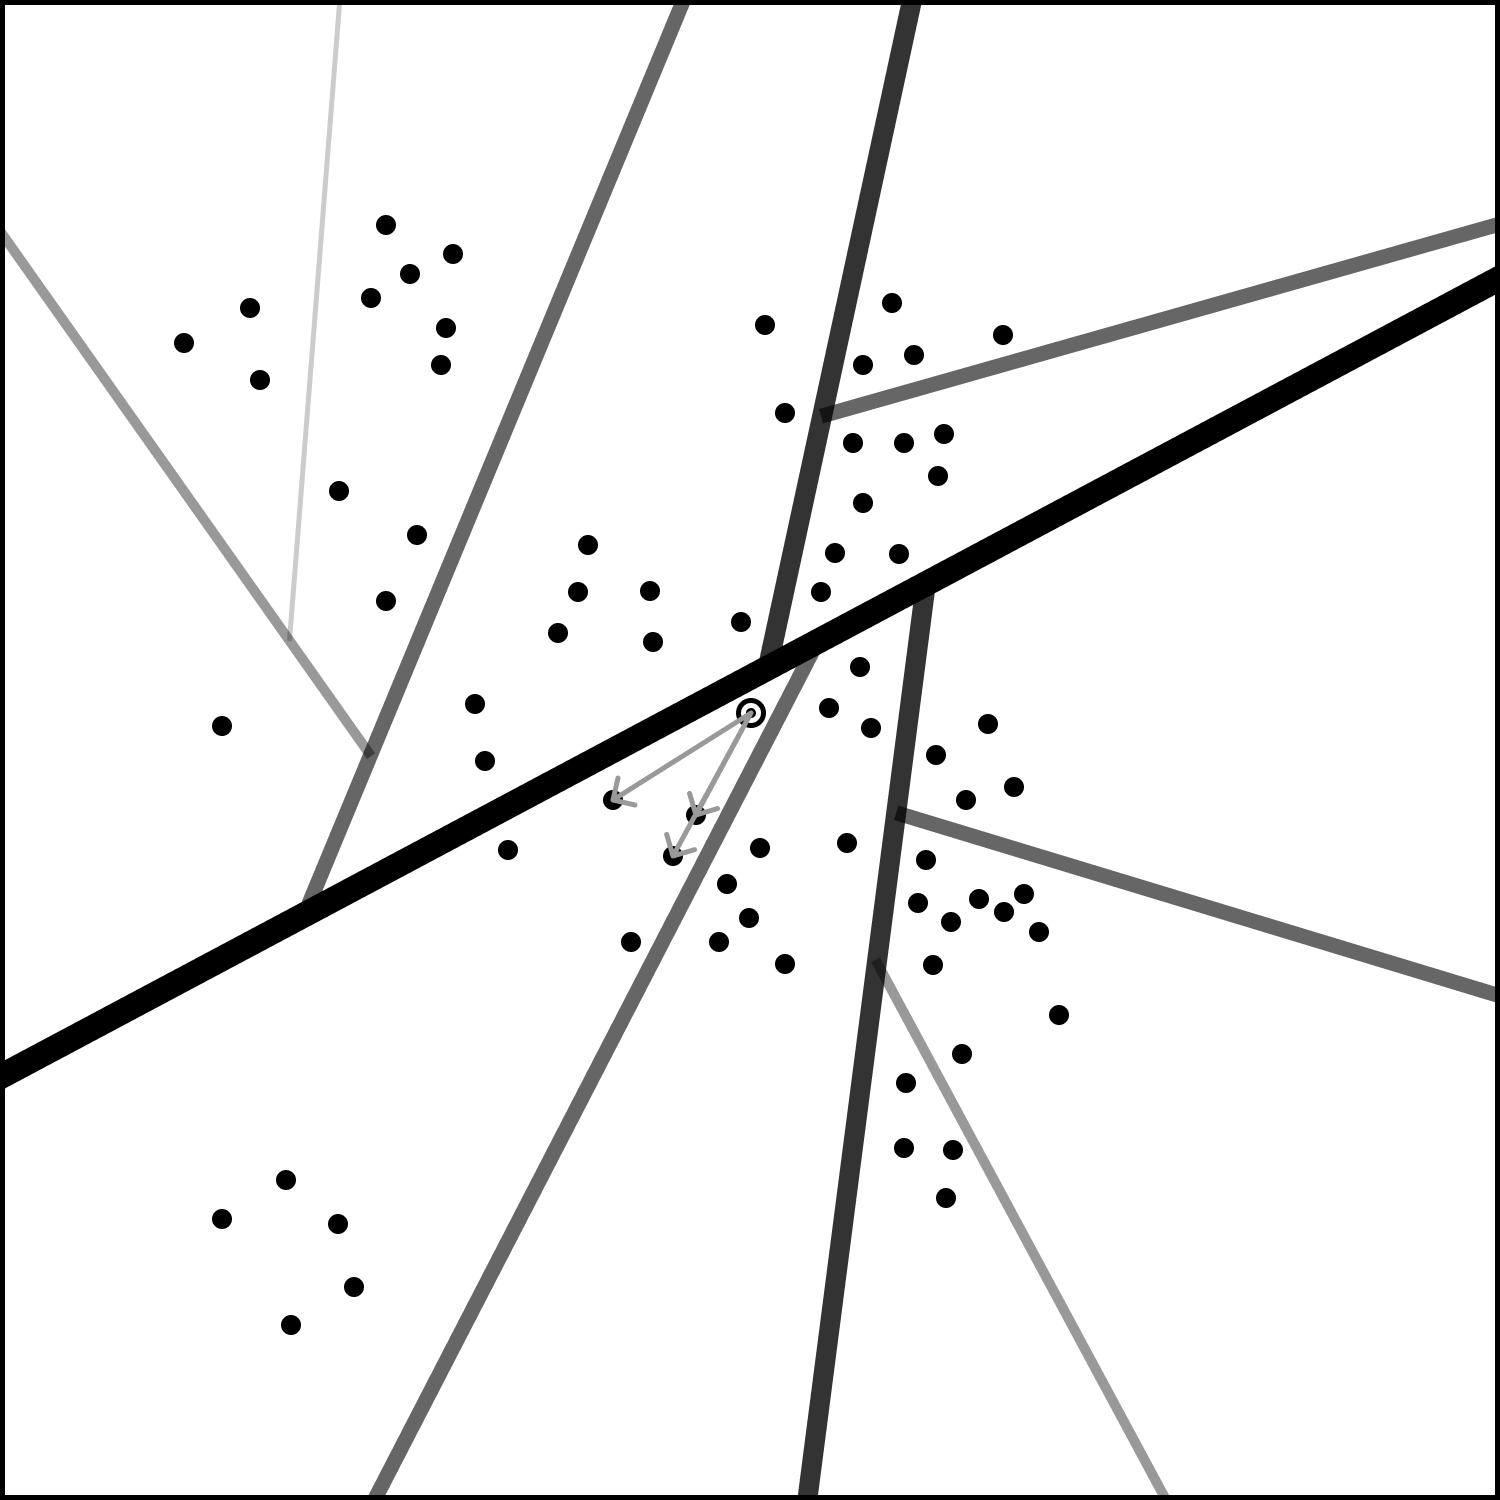
\includegraphics[width=0.48\textwidth]{chapters/algorithms/annoy/figures/query-1.png}
    \caption{Query point within the partitioned space.}
    \label{fig:annoy-5}
\end{figure}

\newpage

\noindent
To perform a query in the structure, the binary tree is traversed from the root (Figure~\ref{fig:annoy-6}). At each step, the query point is assigned to one of the two child nodes depending on which side of the hyperplane it lies. This decision can be made by comparing the distances from the query vector to the two reference vectors used to define the split. Since the height of the tree is logarithmic in the number of points, the traversal can be completed in logarithmic time complexity.

\begin{figure}[H]
    \centering
    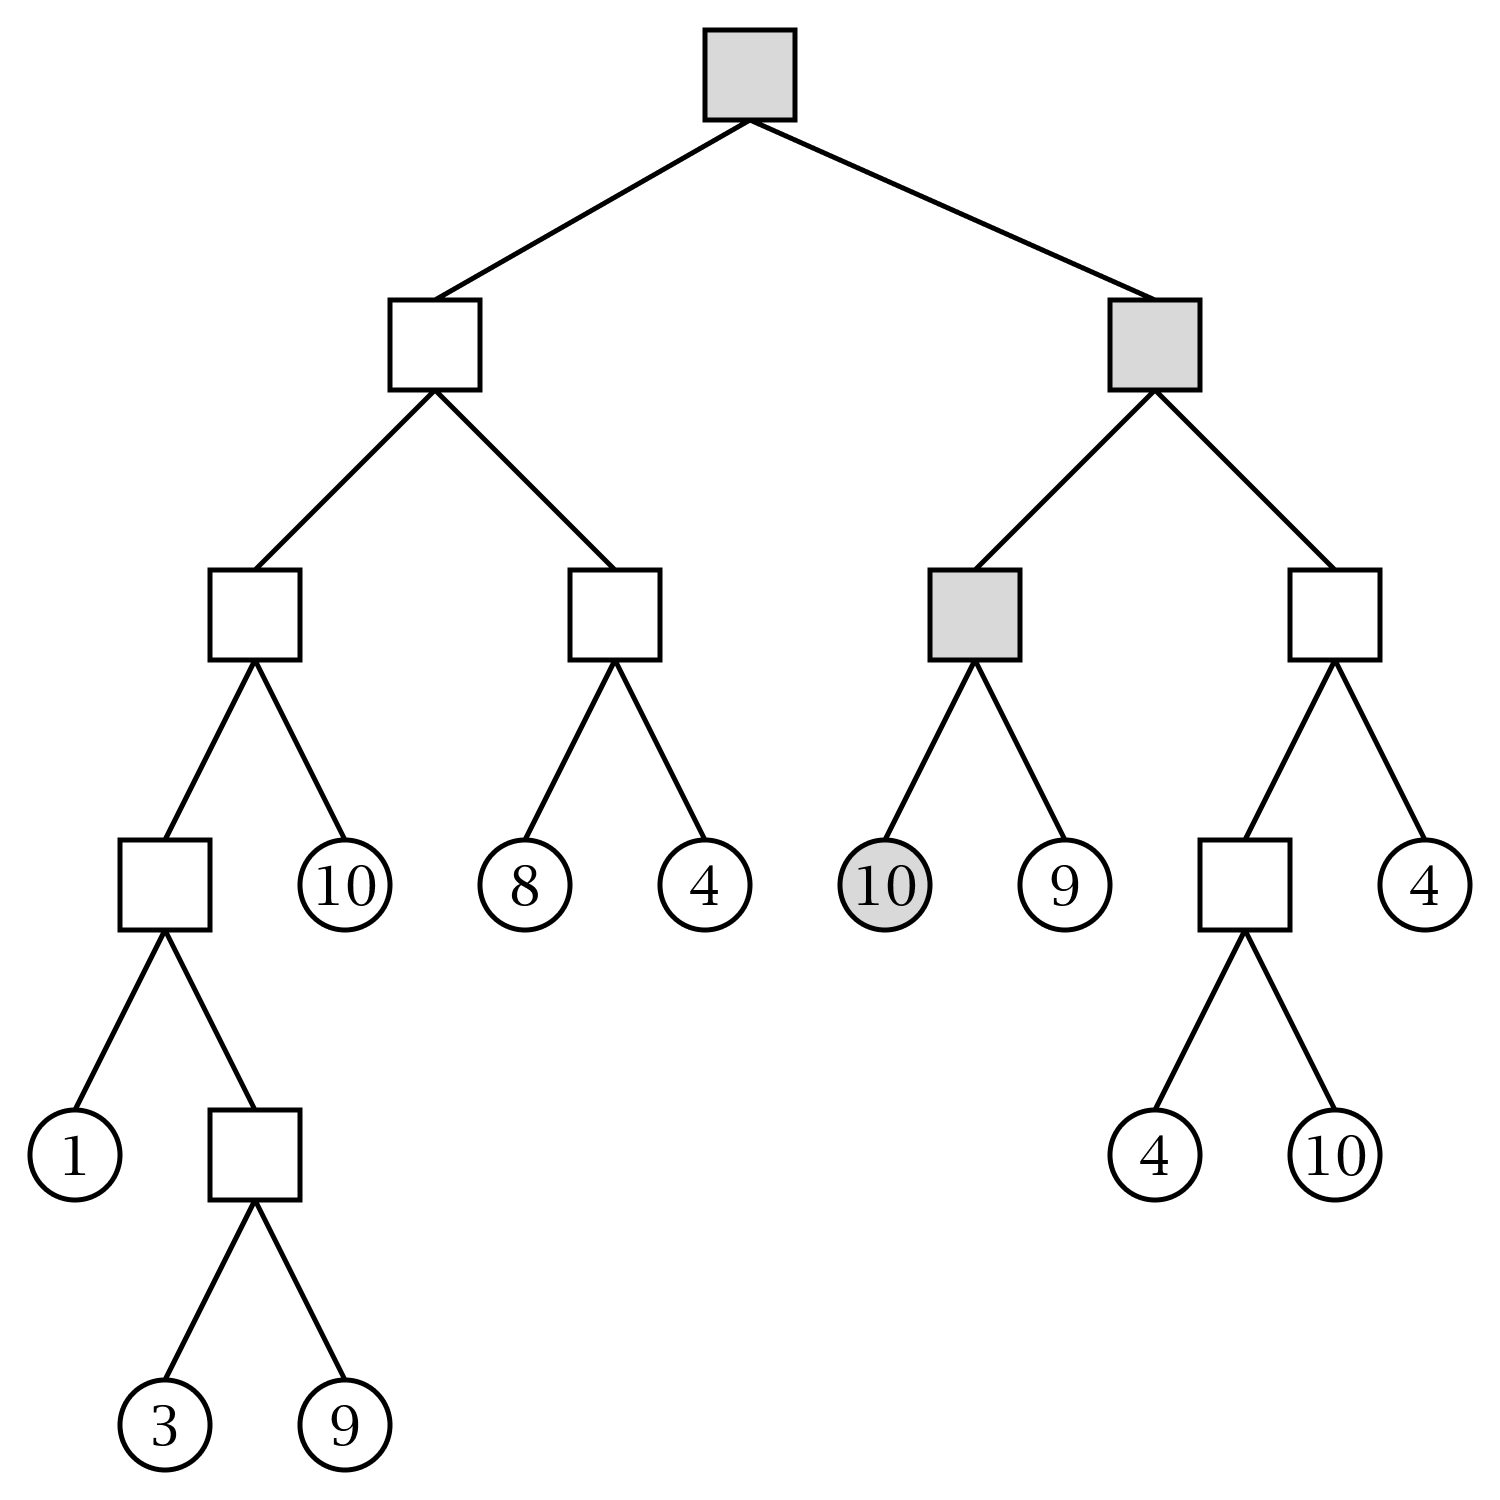
\includegraphics[width=0.48\textwidth]{chapters/algorithms/annoy/figures/traversal-1.png}
    \caption{Traversal path in the binary tree for the query point.}
    \label{fig:annoy-6}
\end{figure}

\noindent
This procedure, however, has two limitations. First, the number of neighbors retrieved is bounded by the capacity of the leaf node, which may be smaller than the desired number of nearest neighbors. Second, some true nearest neighbors may reside outside the leaf region reached by the query, leading to reduced accuracy.

\subsubsection{Indexing: Forest}

\noindent
To mitigate the limitations of individual trees and enhance search accuracy, multiple trees are constructed to form a forest (Figure~\ref{fig:annoy-7}). Each tree is generated independently using a different random set of splits, and a query is evaluated across all trees simultaneously.

\begin{figure}[H]
    \centering
    \begin{subfigure}[t]{0.48\textwidth}
        \centering
        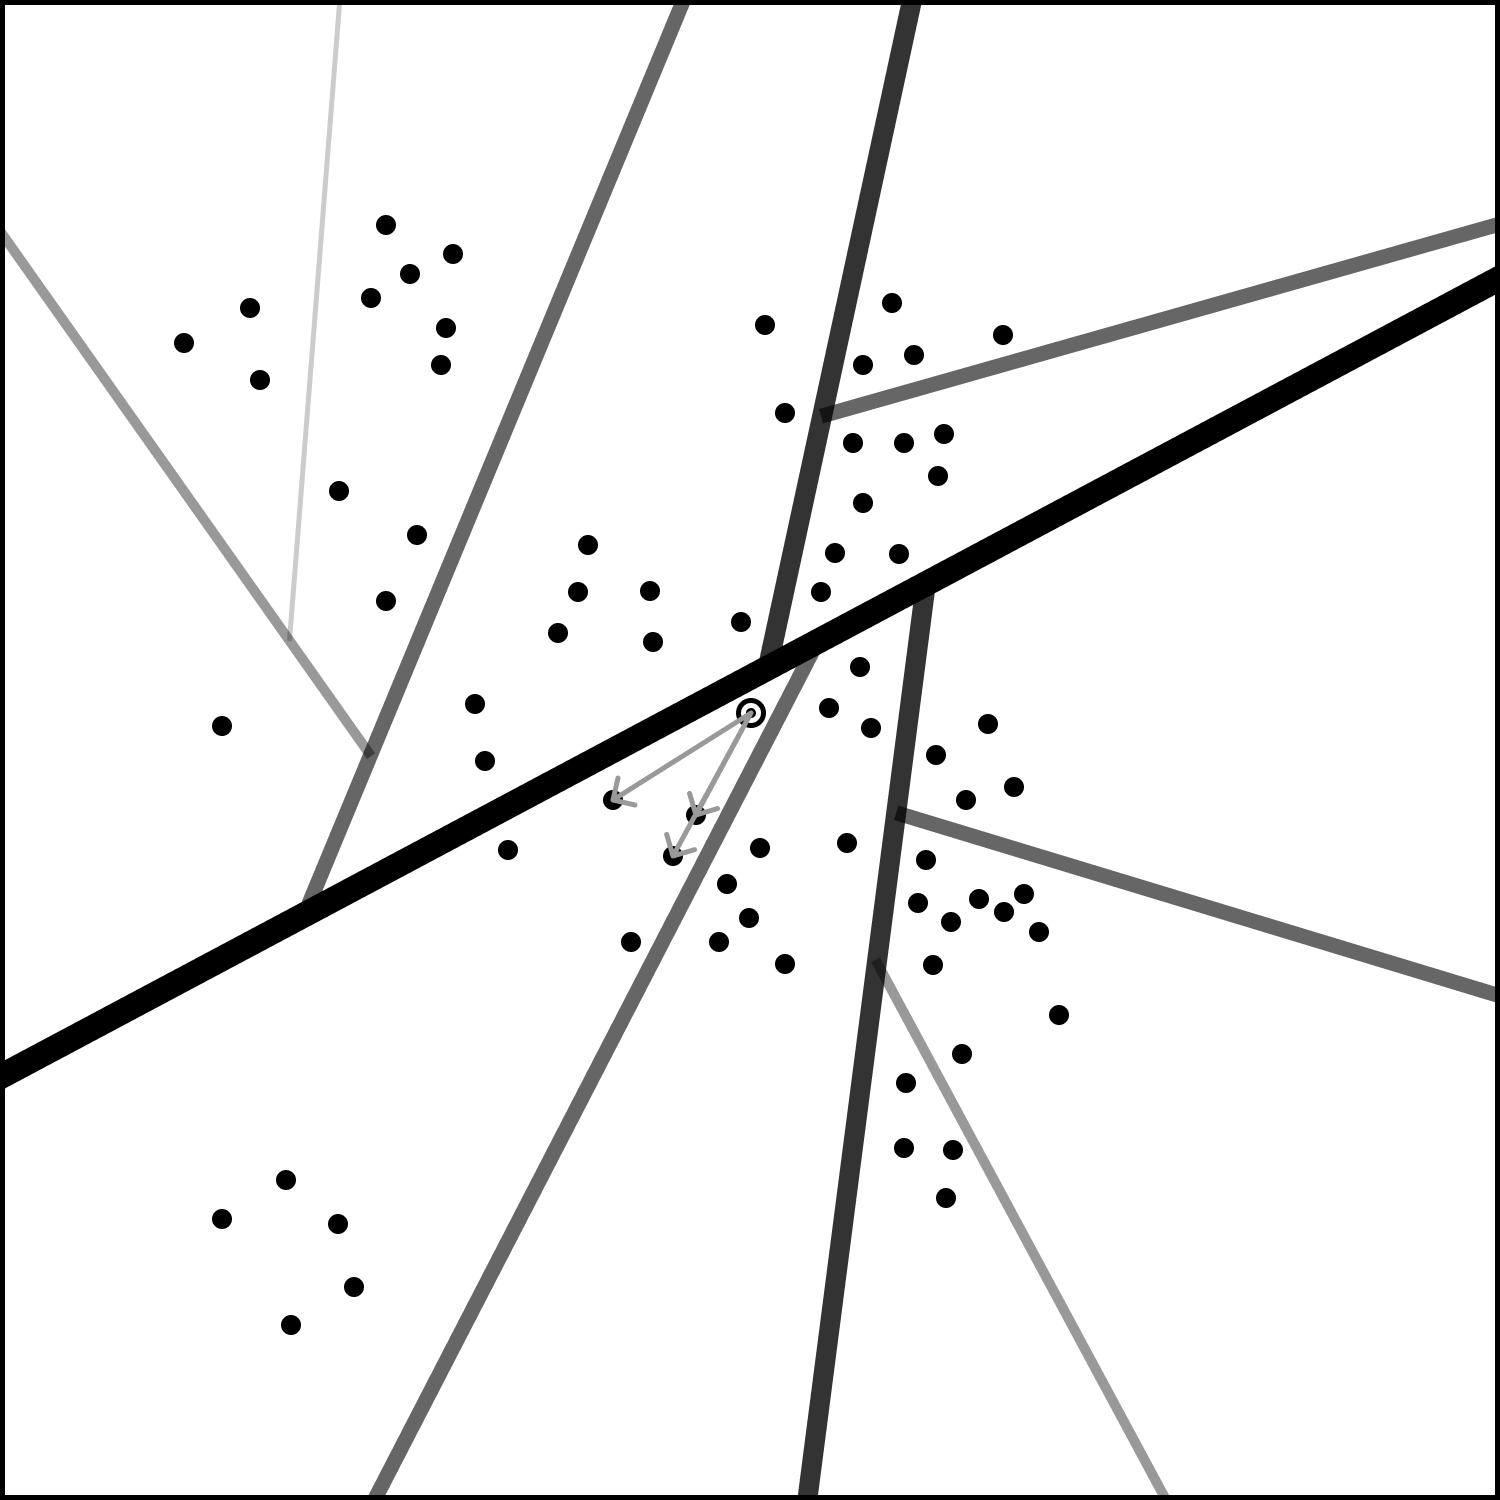
\includegraphics[width=\textwidth]{chapters/algorithms/annoy/figures/query-1.png}
        \caption{Final partitioning of the first tree.}
        \label{fig:annoy-7-a}
    \end{subfigure}
    \hfill
    \begin{subfigure}[t]{0.48\textwidth}
        \centering
        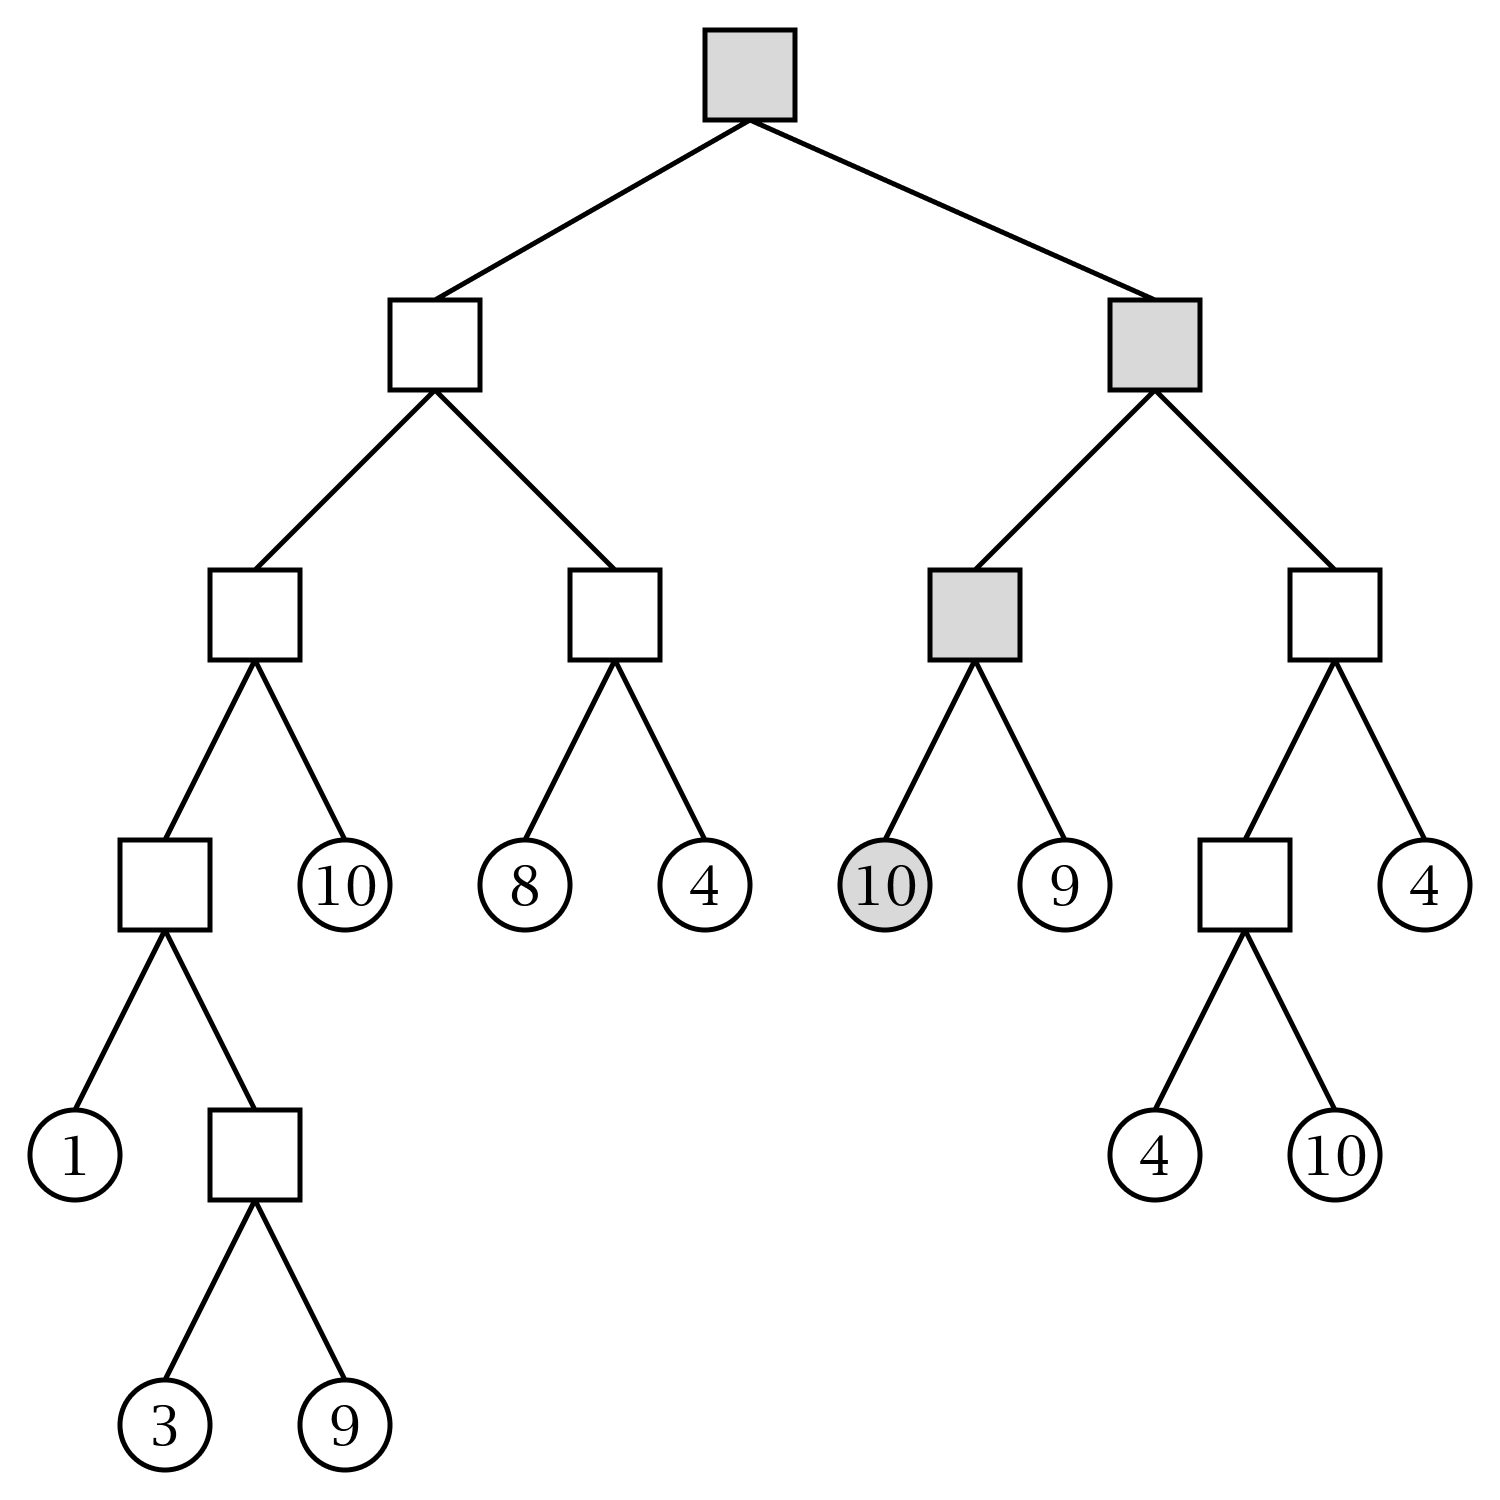
\includegraphics[width=\textwidth]{chapters/algorithms/annoy/figures/traversal-1.png}
        \caption{Binary tree corresponding to the first partitioning.}
        \label{fig:annoy-7-b}
    \end{subfigure}
    
    \vskip 0.3cm
    
    \begin{subfigure}[t]{0.48\textwidth}
        \centering
        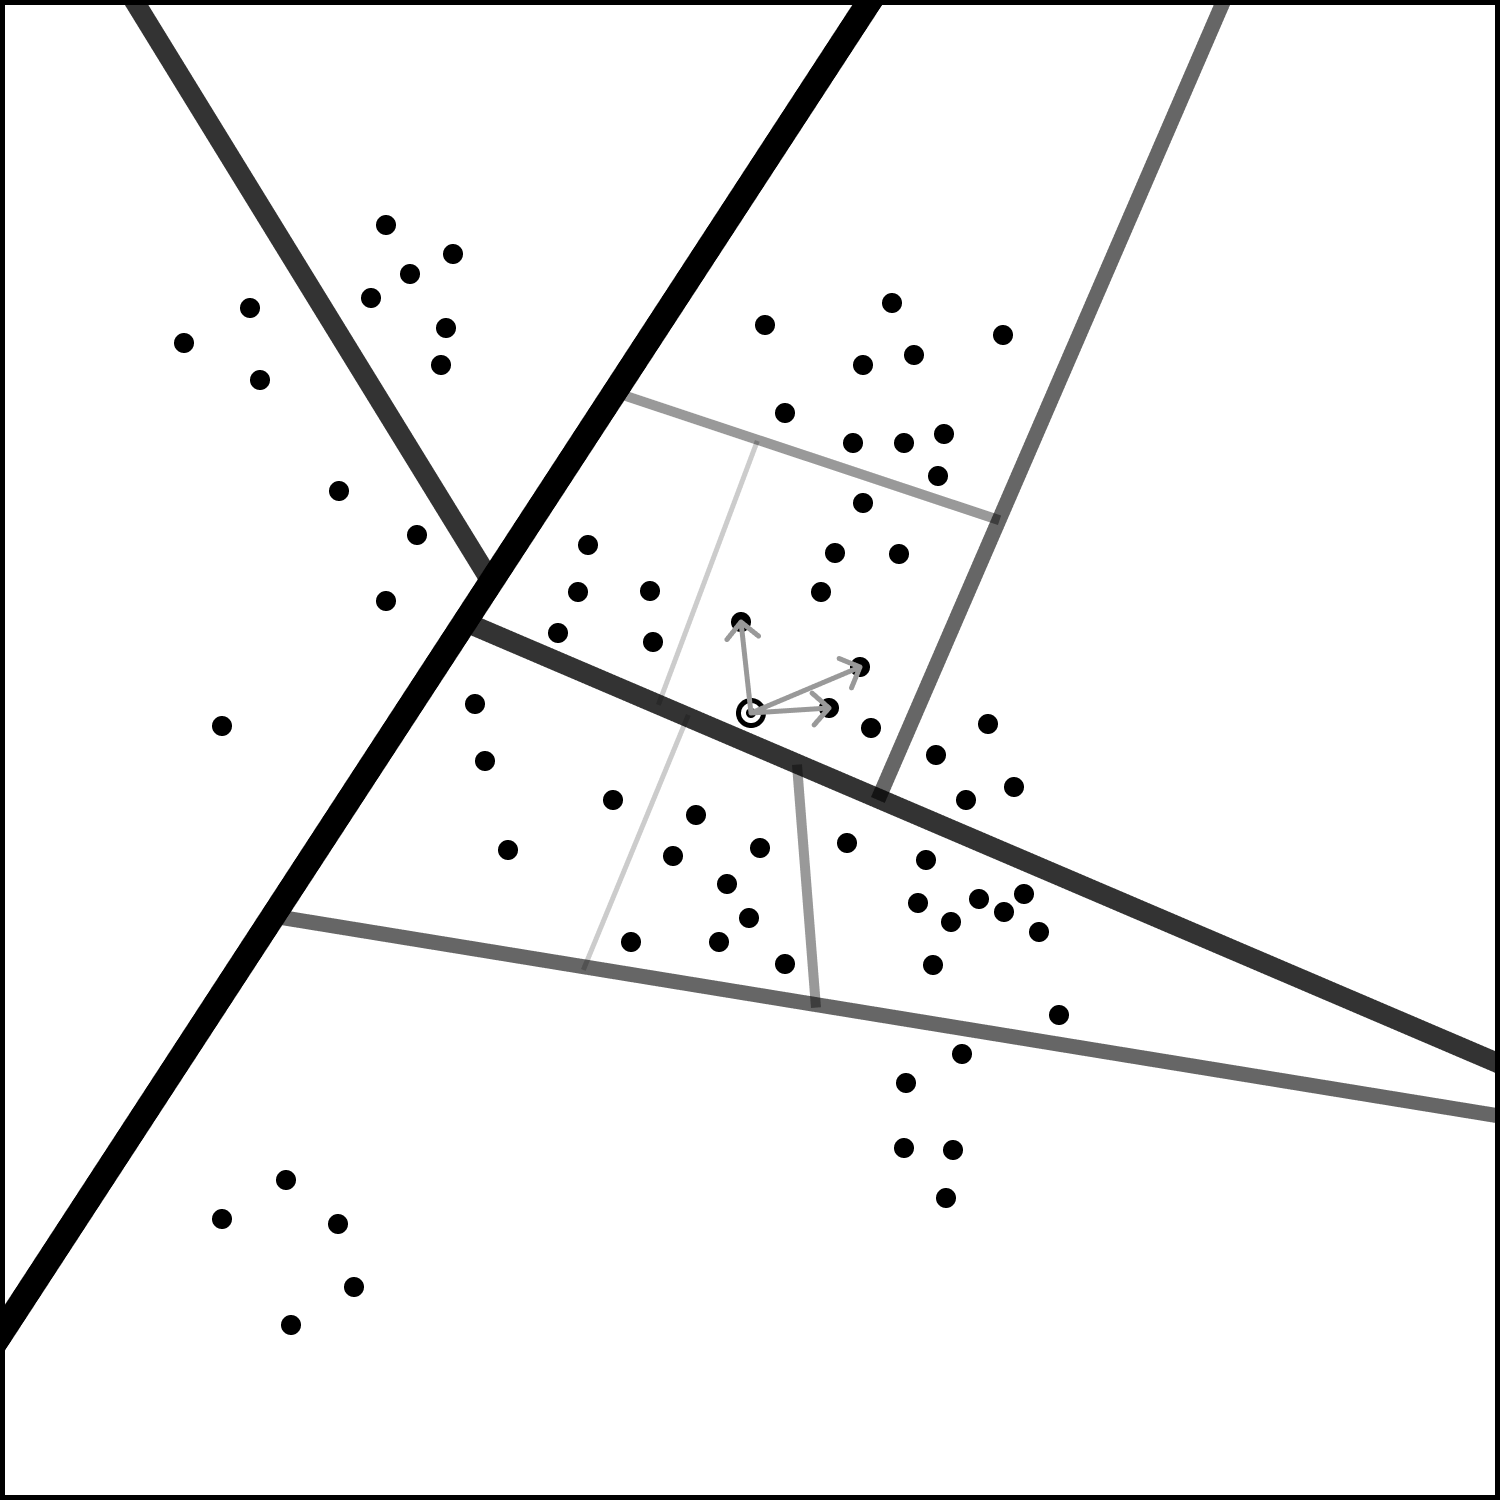
\includegraphics[width=\textwidth]{chapters/algorithms/annoy/figures/query-2.png}
        \caption{Final partitioning of the second tree.}
        \label{fig:annoy-7-c}
    \end{subfigure}
    \hfill
    \begin{subfigure}[t]{0.48\textwidth}
        \centering
        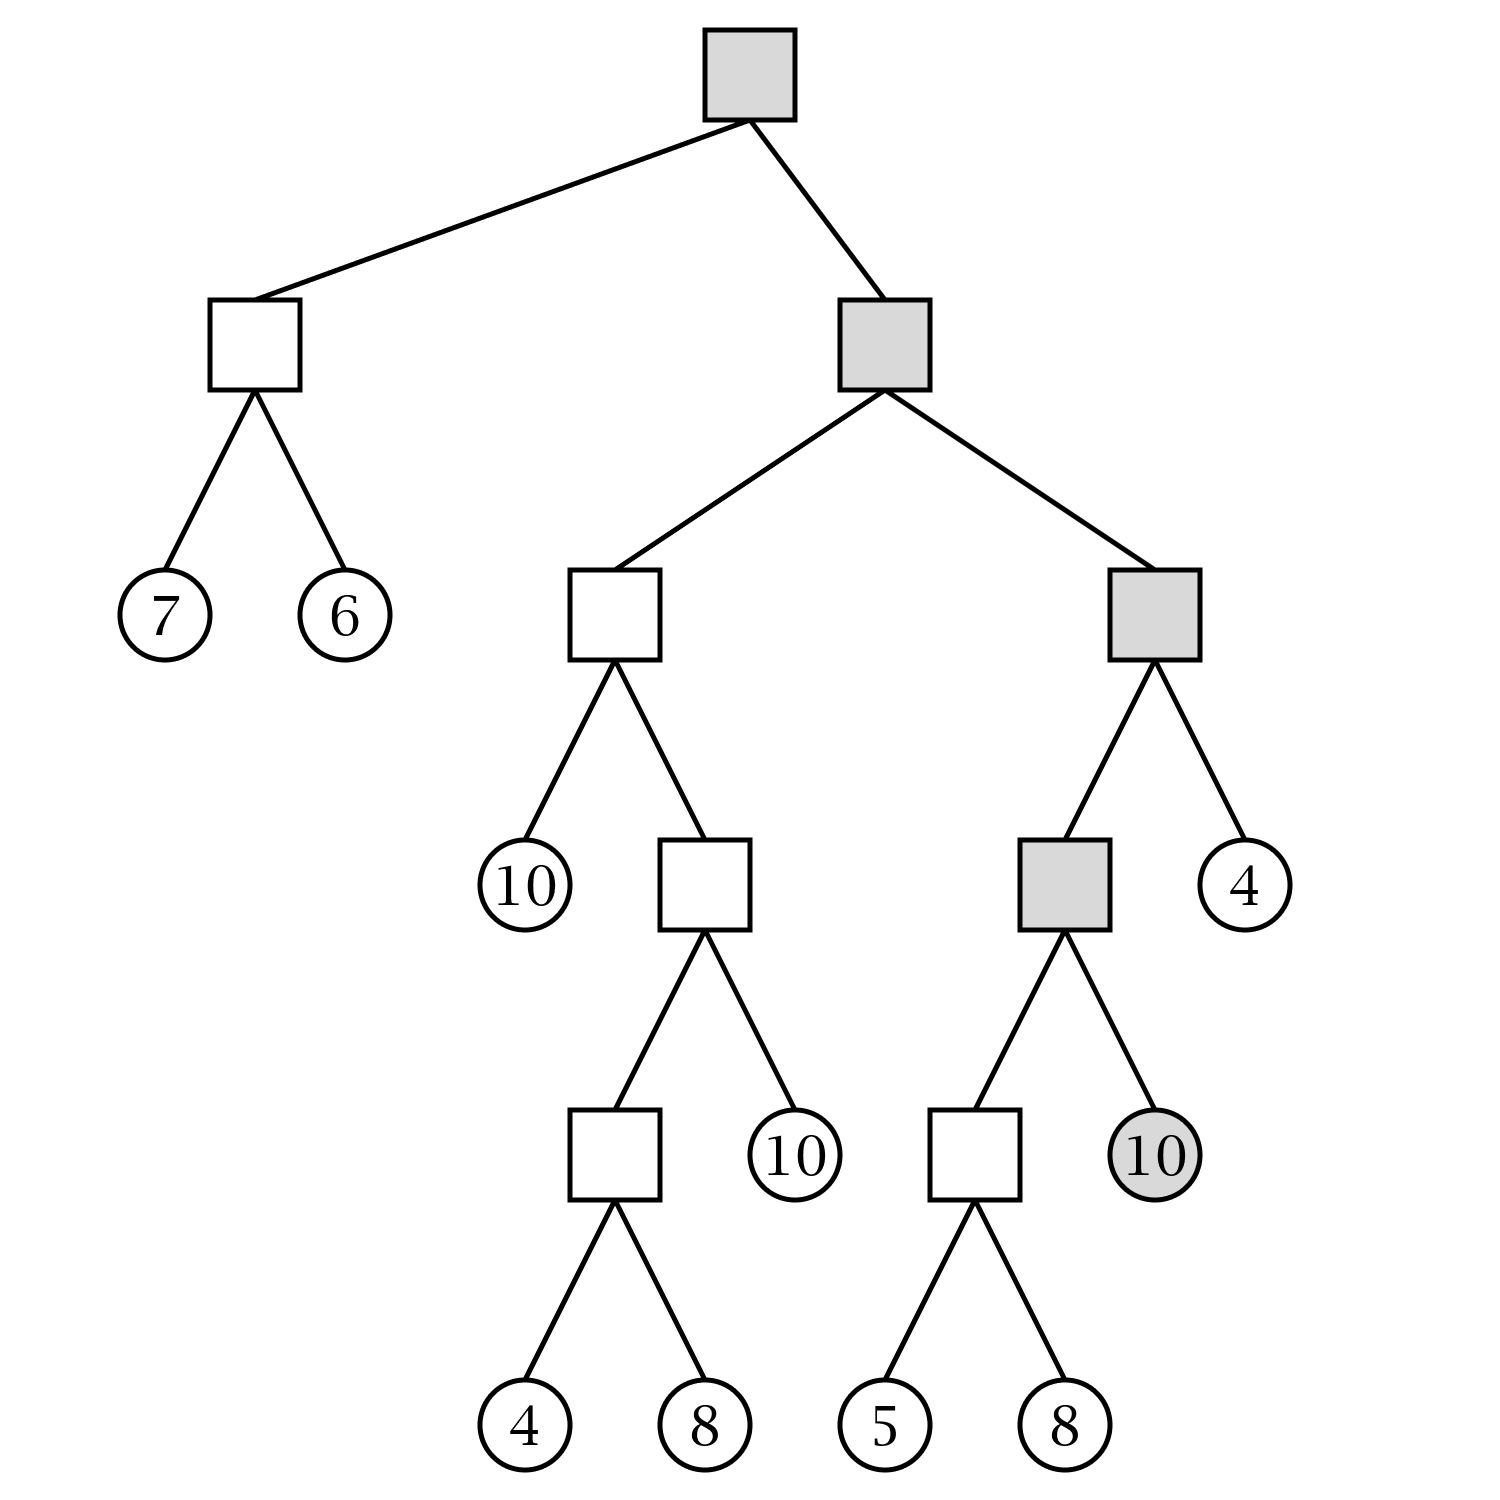
\includegraphics[width=\textwidth]{chapters/algorithms/annoy/figures/traversal-2.png}
        \caption{Binary tree corresponding to the second partitioning.}
        \label{fig:annoy-7-d}
    \end{subfigure}
    
    \caption{Two trees in the Annoy forest. Each tree is generated independently with a random set of splits.}
    \label{fig:annoy-7}
\end{figure}

\noindent
Since each tree contains all points, some points may appear in multiple leaf nodes across different trees. The union of these leaf nodes identifies candidate points that are likely to include the nearest neighbors (Figure~\ref{fig:annoy-8-a}).

Distances from the query point to these candidate points are computed during the simultaneous traversal of all trees, with a single priority queue prioritizing nodes and facilitating retrieval of the top $n$ nearest neighbors (Figure~\ref{fig:annoy-8-b}).

\begin{figure}[H]
    \centering
    \begin{subfigure}[t]{0.48\textwidth}
        \centering
        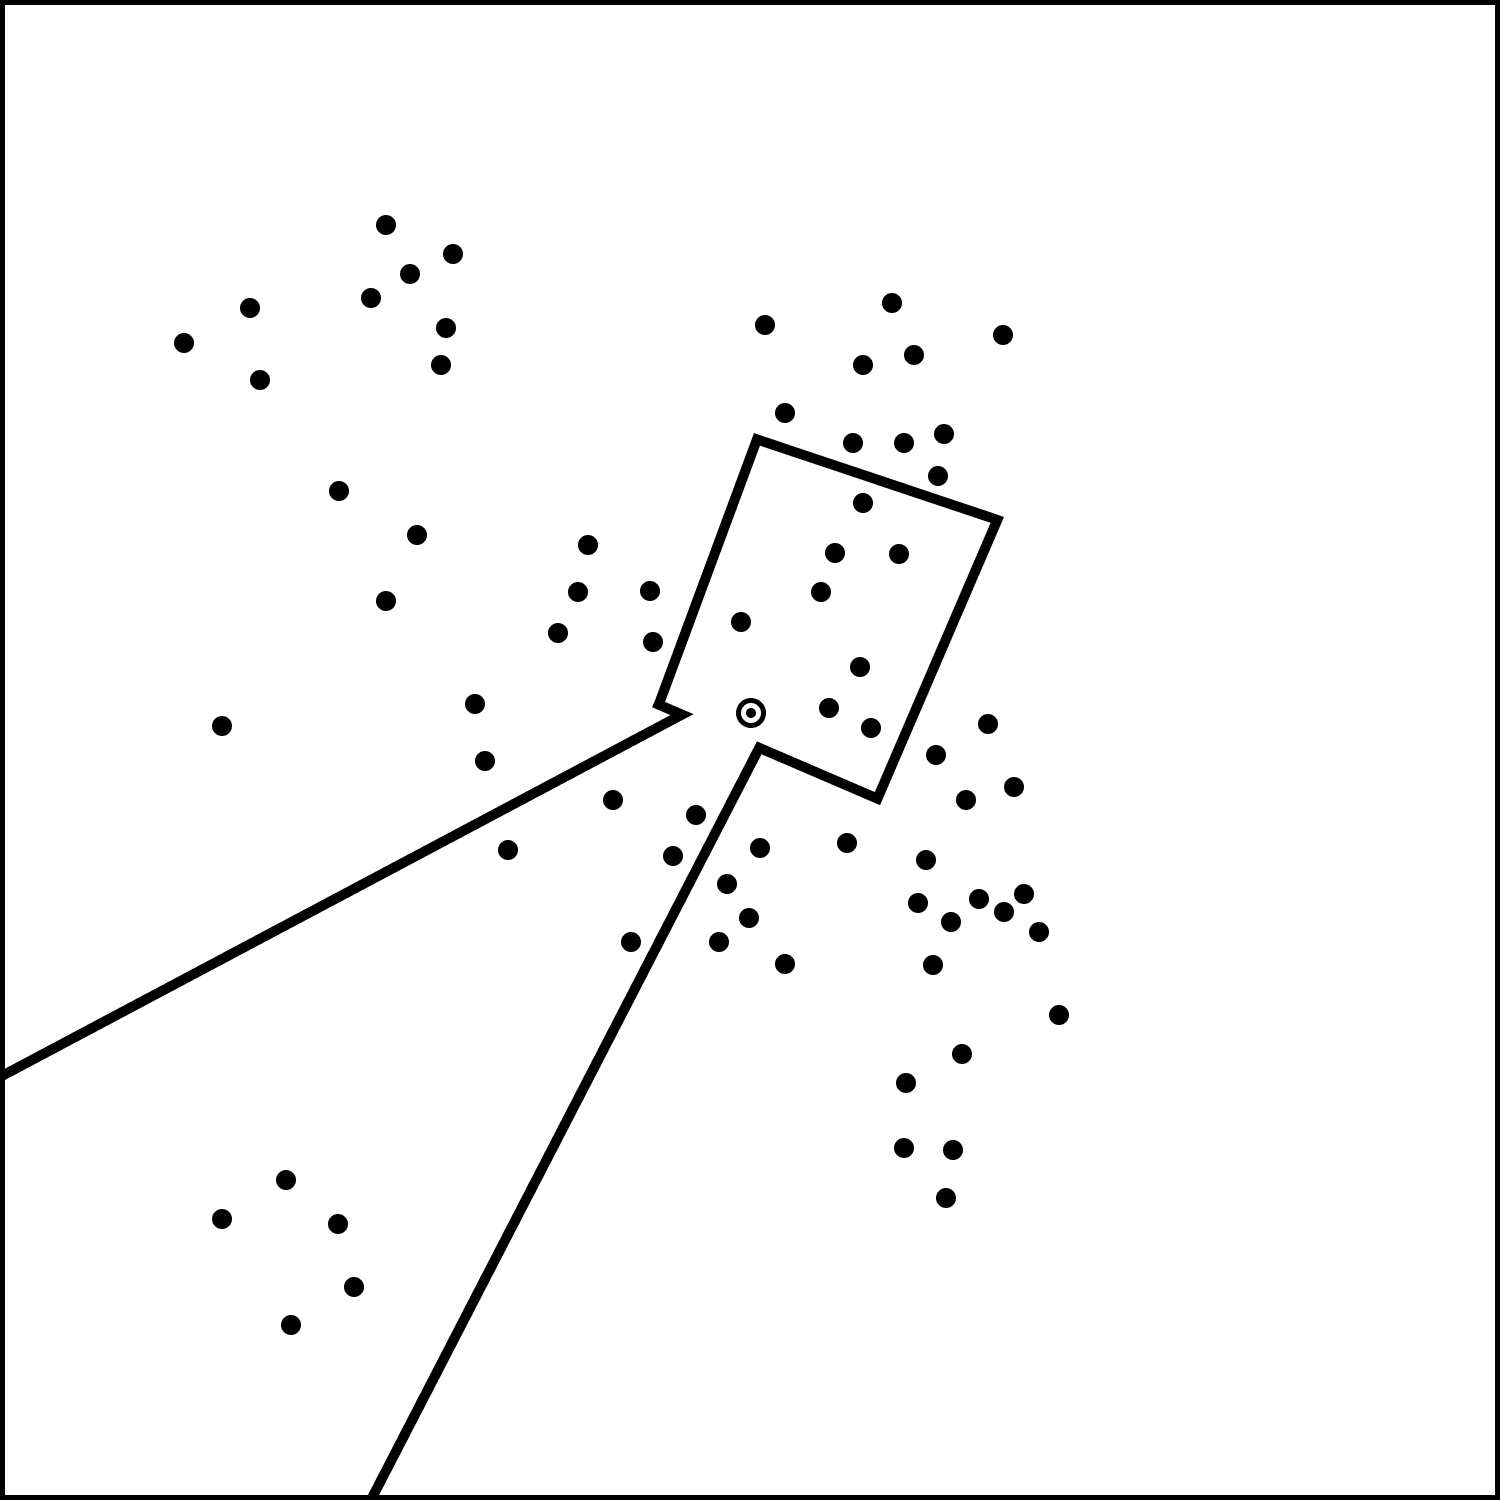
\includegraphics[width=\textwidth]{chapters/algorithms/annoy/figures/union.png}
        \caption{Union of leaf nodes containing the query point across multiple trees in the forest.}
        \label{fig:annoy-8-a}
    \end{subfigure}
    \hfill
    \begin{subfigure}[t]{0.48\textwidth}
        \centering
        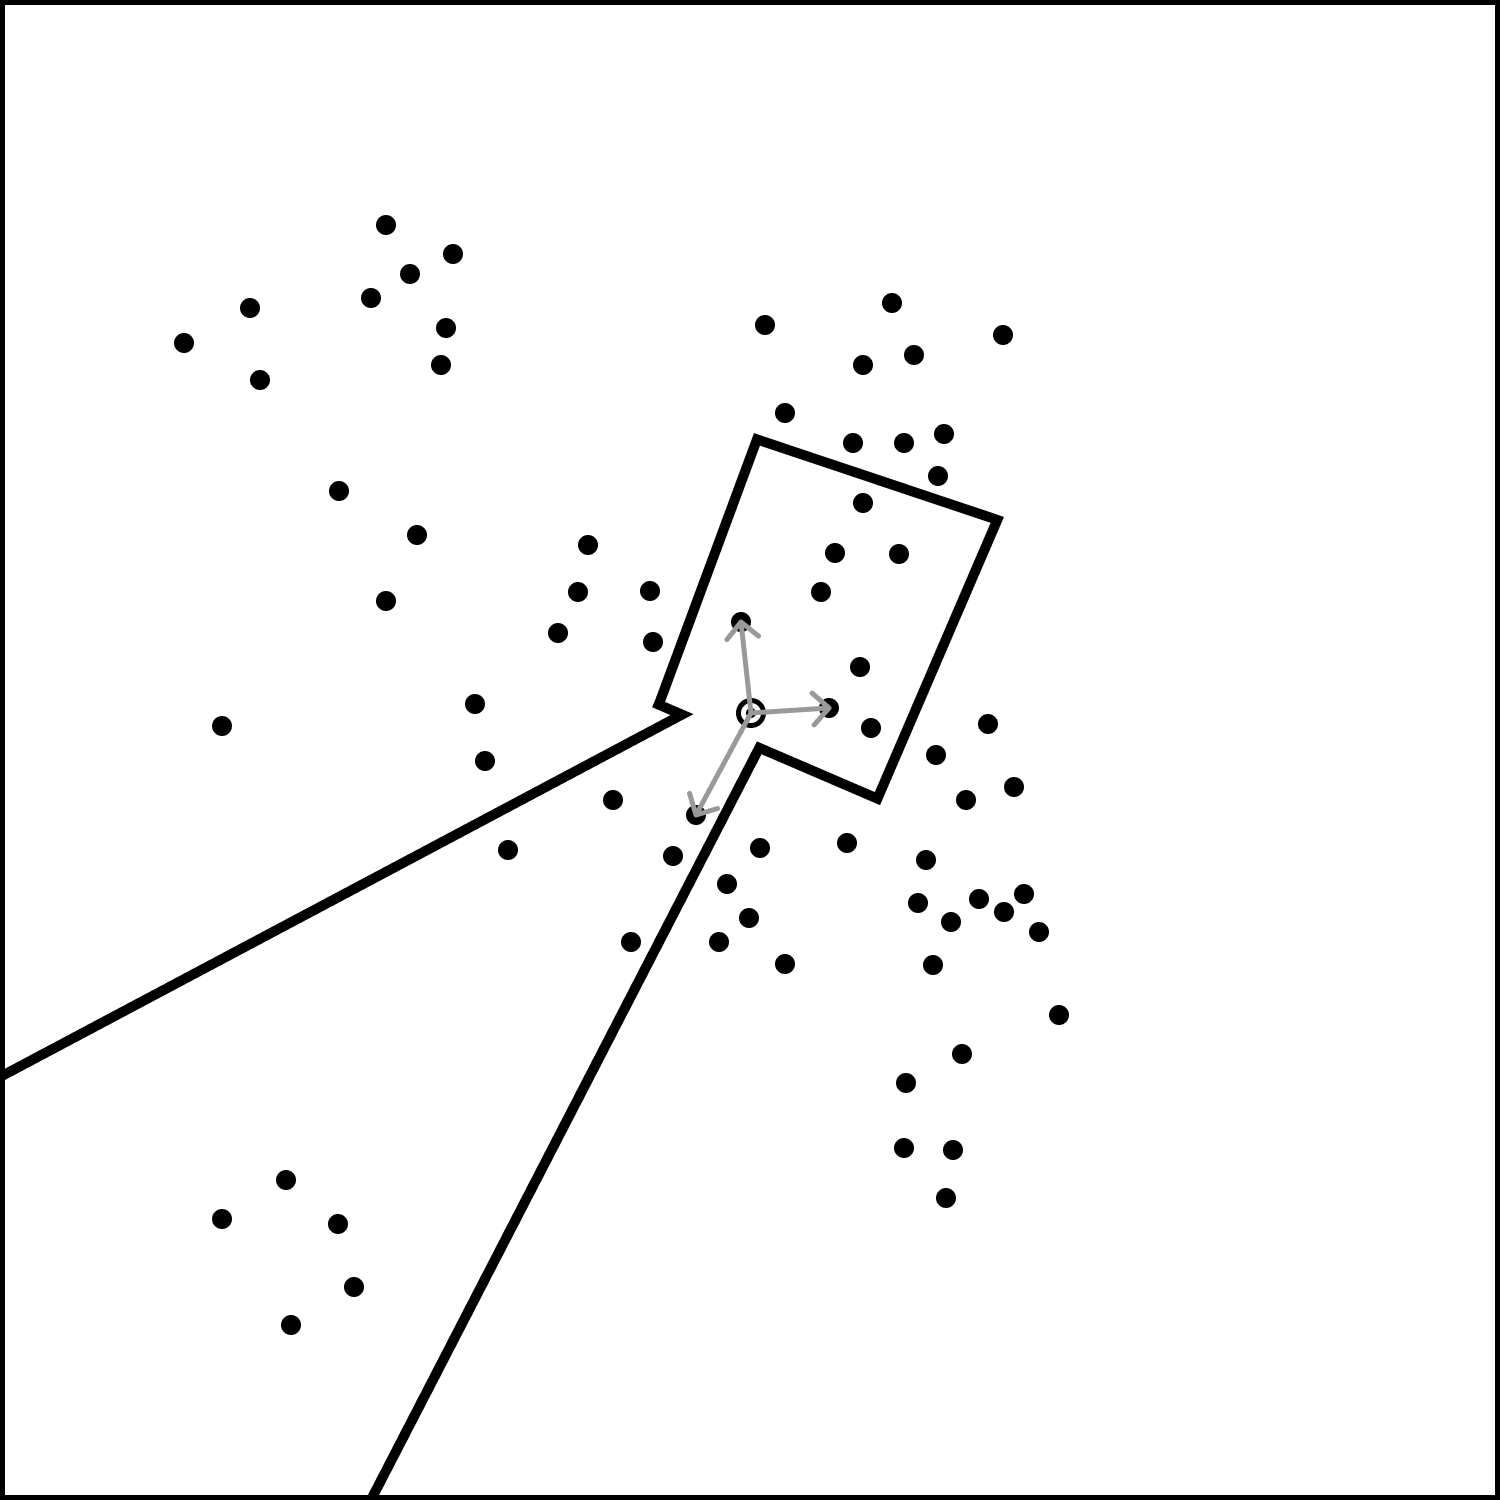
\includegraphics[width=\textwidth]{chapters/algorithms/annoy/figures/distances.png}
        \caption{Distances from the query point to the closest points.}
        \label{fig:annoy-8-b}
    \end{subfigure}
    \caption{Candidate points and distance evaluation during Annoy forest search.}
    \label{fig:annoy-8}
\end{figure}

\noindent
Increasing the number of trees generally improves recall by providing more opportunities to encounter favorable splits. The practical upper limit is typically constrained by available memory resources.

\subsection{Analysis of Annoy}

\subsubsection{Parameters}

There are two main parameters that control the performance of Annoy: the number of trees $n\_trees$ and the number of nodes inspected during query execution $search\_k$ \cite{spotify-annoy}.

\paragraph{$n\_trees$ Parameter}

The parameter $n\_trees$ defines the number of trees in the Annoy forest and is set at build time. Increasing $n\_trees$ generally improves recall, since more independent random partitions raise the chance of obtaining favorable splits. This improvement, however, comes at the cost of longer index construction and increased memory usage. In practice, the value of $n\_trees$ is typically chosen as large as possible within available memory limits \cite{spotify-annoy}.

\paragraph{$search\_k$ Parameter}

The parameter $search\_k$ specifies the number of nodes inspected during query execution and is set at runtime. Larger values improve recall by considering more candidate points, but also increase query latency. If not explicitly specified, $search\_k$ defaults to $n \times n\_trees$, with $n$ denoting the number of requested nearest neighbors. In practice, $search\_k$ is usually set as large as possible given the time constraints for query processing \cite{spotify-annoy}.

\subsubsection{Multiple Processes and Memory Sharing}

A distinctive feature of Annoy is its ability to share a single index across multiple processes. This is achieved by creating static file-based indexes that can be memory-mapped (mmap) by any number of processes. By decoupling index creation from loading, the same index file can be distributed or passed around, allowing immediate lookups without rebuilding the structure.

This approach is particularly useful in high-performance or distributed environments, where multiple CPUs or workers need to access the index concurrently. Only a single copy of the index needs to be built, minimizing both construction overhead and memory usage. Moreover, because index creation is separate from lookup, no additional vectors can be added once the index is built \cite{spotify-annoy}.
\section{Hierarchical Navigable Small World (HNSW)}

\subsection{Introduction to HNSW}

Hierarchical Navigable Small World (HNSW) is a graph-based approach for approximate nearest neighbor (ANN) search, built on navigable small-world (NSW) networks with a controllable hierarchical structure. It was initially introduced by Malkov and Yashunin as an arXiv preprint in 2016 \cite{Malkov-Yashunin-2016} and later published in the peer-reviewed \textit{IEEE Transactions on Pattern Analysis and Machine Intelligence} in 2020 \cite{Malkov-Yashunin-2020}.

HNSW incrementally builds a multi-layered structure composed of hierarchical proximity graphs, where each layer corresponds to a nested subset of the stored elements. The maximum layer in which an element appears is selected randomly according to an exponentially decaying probability distribution \cite{Malkov-Yashunin-2016}.

Starting the search from the upper layer, together with utilizing scale separation, boosts performance compared to NSW and allows logarithmic complexity scaling \cite{Malkov-Yashunin-2016}. Performance evaluations have shown that HNSW remains one of the state-of-the-art approaches for vector search \cite{erikbern-ann-benchmarks}, leading to its adoption in various vector databases and search systems.

The HNSW implementation is available at GitHub\footnote{\url{https://github.com/nmslib/hnswlib}}.

\subsection{Building Blocks of HNSW}

\subsubsection{Navigable Small World (NSW)}

Navigable Small World (NSW), predecessor of HNSW, is a graph-based approach for approximate nearest neighbor (ANN) search. It combines two key ideas: short-range connections that approximate the Delaunay triangulation, and long-range connections that ensure the small-world navigation property (Figure~\ref{fig:hnsw-1} \cite{Malkov-Ponomarenko-Logvinov-Krylov-2014}). The short-range edges preserve local proximity information required for greedy search, while long-range edges maintain overall graph connectivity and enable polylogarithmic scalability of search complexity. A distinctive feature of the NSW construction is that long-range links arise naturally: as new elements are inserted consecutively and connected to their nearest neighbors, some of the previously added edges gradually become long-range connections \cite{Malkov-Ponomarenko-Logvinov-Krylov-2014}.

An important limitation of NSW lies in its routing process, which can be divided into two phases: "zoom-out" and "zoom-in" \cite{Malkov-Yashunin-2016}. In the "zoom-out" phase, the search expands outward from a low-degree node, progressively reaching high-degree nodes (hubs), while in the "zoom-in" phase the routing converges towards the target through increasingly local, short-range connections \cite{Boguna-Krioukov-Claffy-2007}. Starting the search directly from hubs, thereby skipping the "zoom-out" stage, reduces the probability of getting stuck in a distant false local minimum and improves efficiency. Nevertheless, the overall routing in NSW still exhibits only polylogarithmic complexity. This shortcoming motivated the introduction of a hierarchical structure in HNSW to achieve logarithmic search complexity \cite{Malkov-Yashunin-2016}.

\begin{figure}[H]
    \centering
    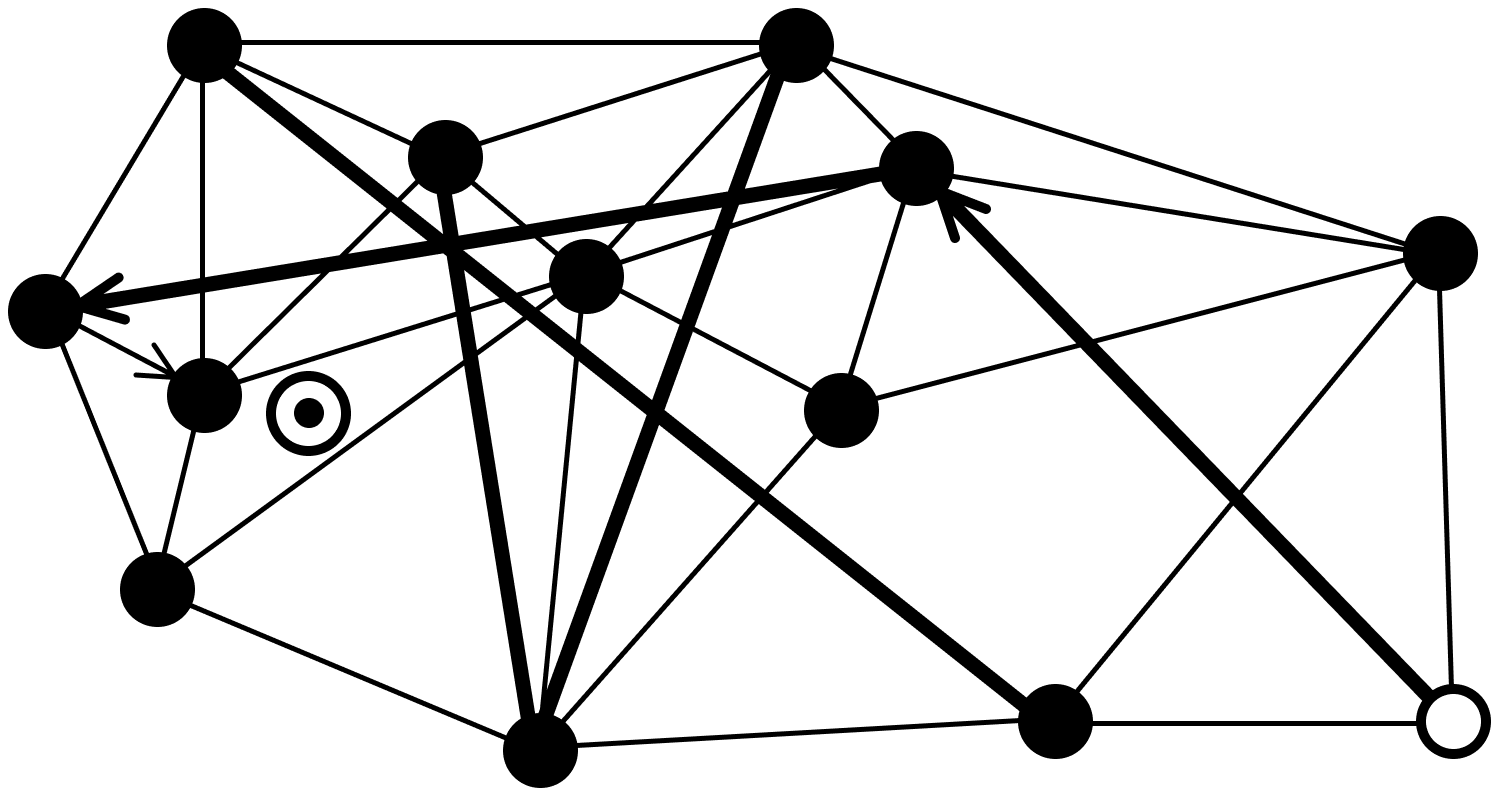
\includegraphics[width=0.6\textwidth]{chapters/algorithms/hnsw/figures/nsw.png}
    \caption{Graph representation of an NSW structure. Filled circles represent data points, while the entry point and the query point are indicated as an empty circle and a target circle, respectively. Thin edges represent short-range connections preserving local proximity, and thick edges represent long-range connections ensuring overall graph connectivity and enabling polylogarithmic search complexity. Arrows illustrate the path of the greedy search from the entry point to the query.}
    \label{fig:hnsw-1}
\end{figure}

\paragraph{The Small World Problem}

Social psychologist Milgram investigated \cite{Milgram-1967} how individuals are connected into social networks through ties of kinship and acquaintance, and whether short paths exist between any two randomly chosen people. To test this, he devised an experimental method: participants were given the name and basic information of a target person. If they did not personally know the target, they were instructed to forward the folder to a personal acquaintance who was more likely to know the target, restricted to contacts they knew on a first-name basis.

The experiment revealed that the median number of intermediaries required to connect two individuals was approximately 5.5, providing empirical evidence for the small-world phenomenon (popularly known as \textit{six degrees of separation} \cite{Guare-1990}).

\subparagraph{Navigability}

Computer scientist Kleinberg studied \cite{Kleinberg-2000-5, Kleinberg-2000-8} how individuals can efficiently find short paths in large social networks using only local information. He modeled networks following the small-world paradigm, characterized by dense short-range connections and a few random long-range links. While small-world networks guarantee that short paths exist between any two nodes, this does not ensure that a decentralized algorithm can discover them.

Kleinberg showed that there exists a unique value of a parameter controlling the distribution of long-range links at which a greedy algorithm can navigate efficiently, with expected delivery time scaling polylogarithmically with $N$, where $N$ is the number of nodes. For other values of this parameter, navigation becomes asymptotically inefficient. These results indicate that navigability is not a general property of all small-world networks but only emerges under specific structural conditions.

\paragraph{Proximity Graph}

Proximity graphs are geometric graphs in which two vertices $p$ and $q$ are connected by an edge $(p, q)$ if and only if a certain exclusion region defined for $p$ and $q$ contains no other points from the vertex set. Depending on the choice of the exclusion region, various types of proximity graphs can be defined, such as the Delaunay triangulation \cite{Mitchell-Mulzer-2017}.

\newpage

\subparagraph{Voronoi Diagram}

Given a set of points in the plane (Figure~\ref{fig:hnsw-2-a} \cite{Moghaddam-Banihashemi-Bakhshoodeh-Mir-Delgado-2023}), a Voronoi diagram partitions the plane according to the nearest-neighbor rule: each point is associated with the region of the plane that is closest to it (Figure~\ref{fig:hnsw-2-b} \cite{Moghaddam-Banihashemi-Bakhshoodeh-Mir-Delgado-2023}). Voronoi diagrams naturally arise in various proximity problems, such as the classical post-office problem, which asks how a fixed set of points can be preprocessed to quickly determine the nearest point to an arbitrary query location, and its generalization to finding the $k$ nearest points \cite{Aurenhammer-1991}.

\begin{figure}[H]
    \centering
    \begin{subfigure}[t]{0.48\textwidth}
        \centering
        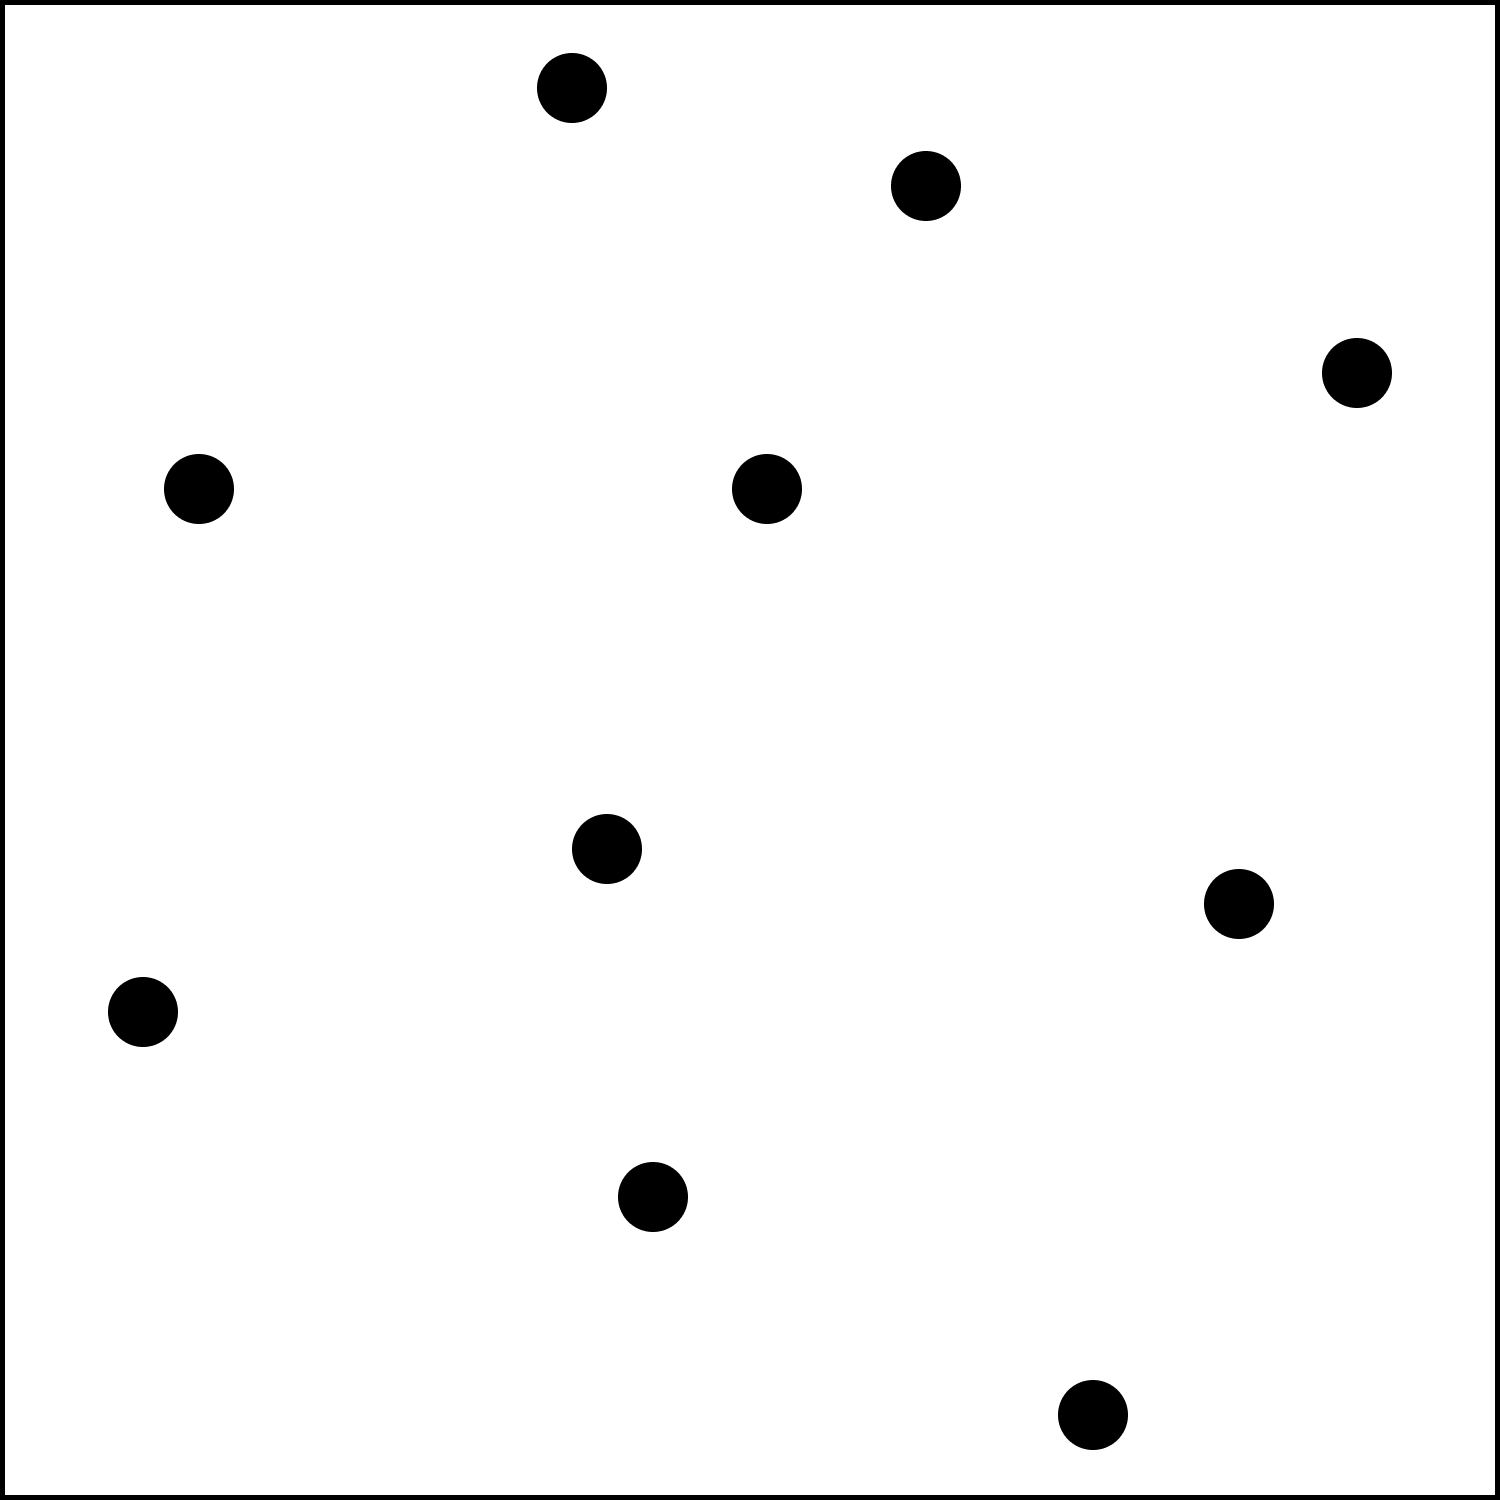
\includegraphics[width=\textwidth]{chapters/algorithms/hnsw/figures/voronoi-points.png}
        \caption{Data points in the plane.}
        \label{fig:hnsw-2-a}
    \end{subfigure}
    \hfill
    \begin{subfigure}[t]{0.48\textwidth}
        \centering
        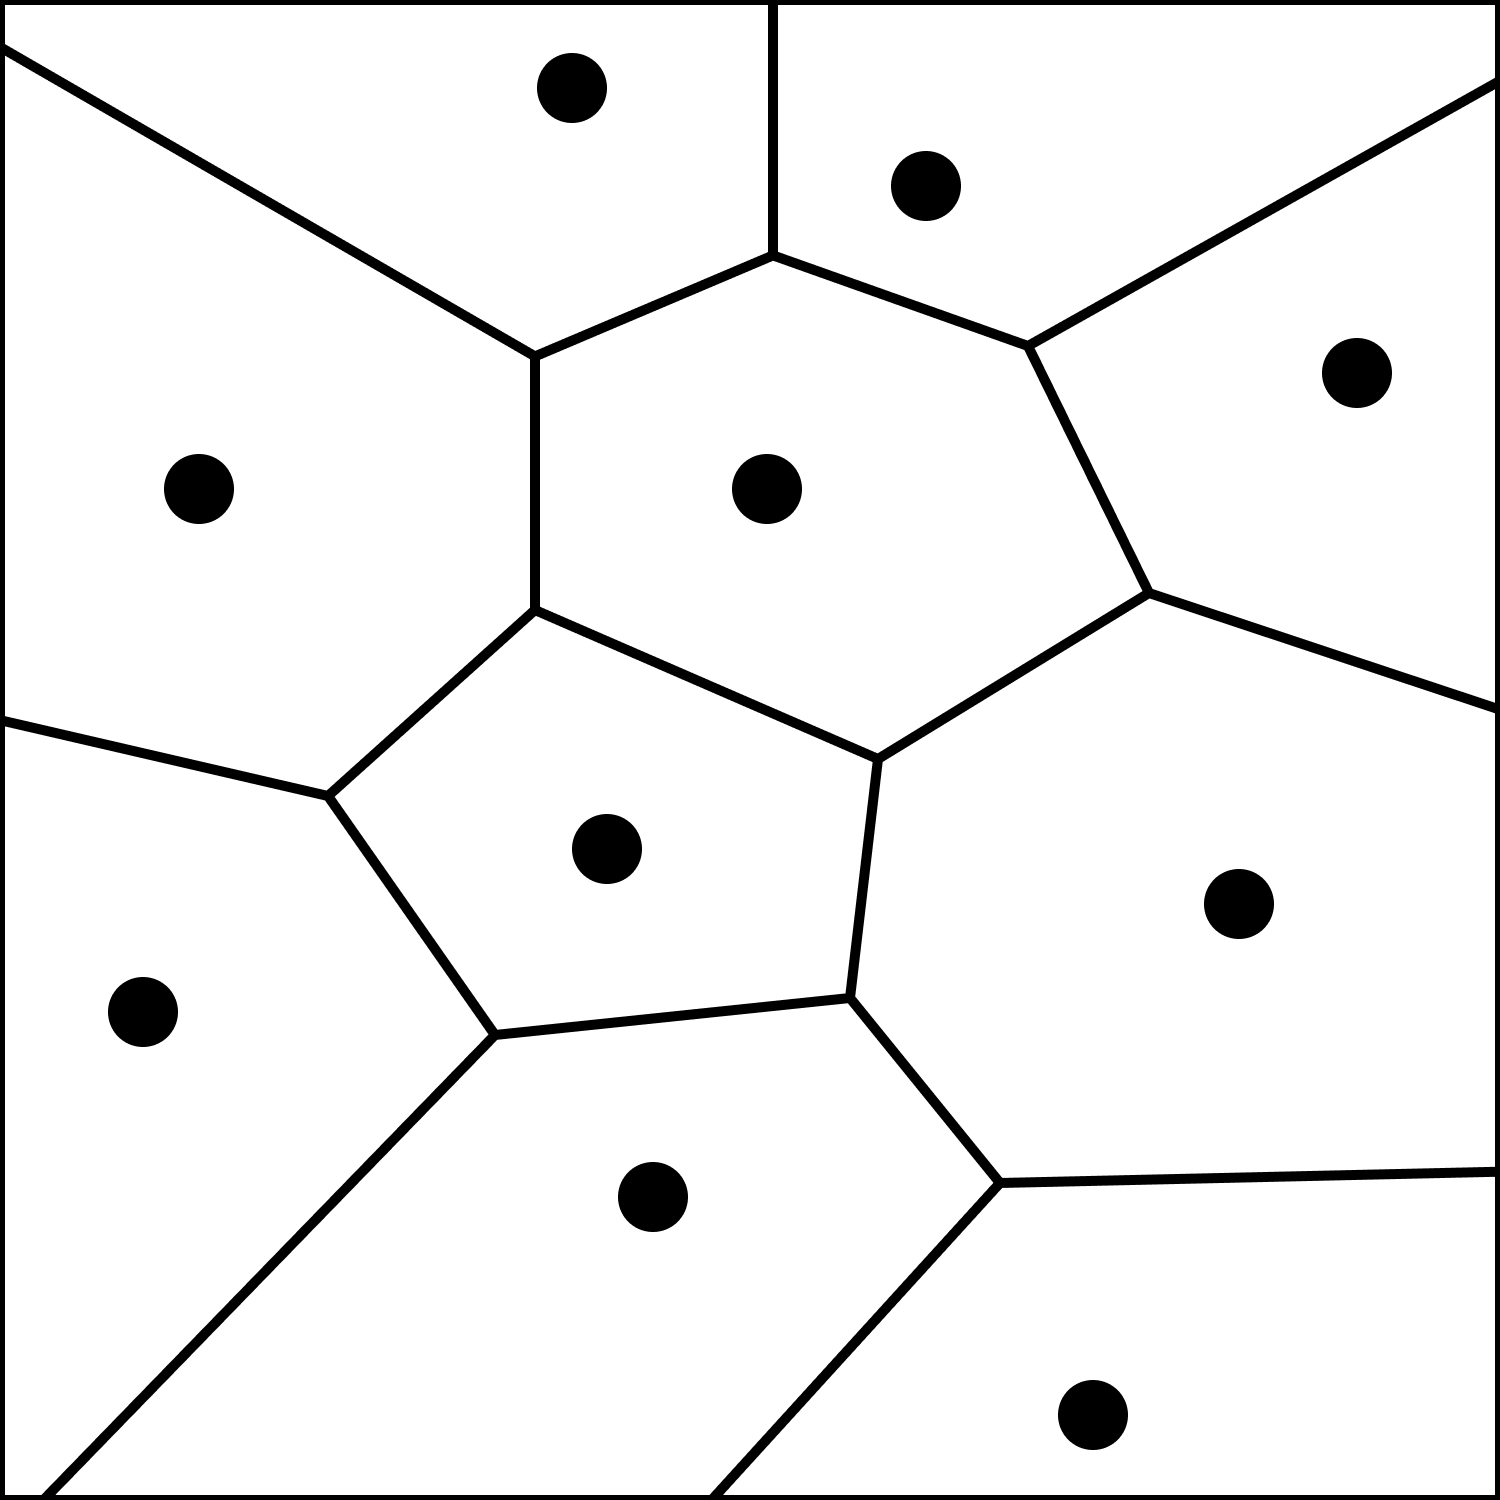
\includegraphics[width=\textwidth]{chapters/algorithms/hnsw/figures/voronoi-diagram.png}
        \caption{Voronoi diagram of the points, showing nearest-neighbor regions.}
        \label{fig:hnsw-2-b}
    \end{subfigure}
    \caption{Voronoi diagram illustration: (a) data points, (b) nearest-neighbor partitioning of the plane.}
    \label{fig:hnsw-2}
\end{figure}

\subparagraph{Delaunay Triangulation}

Delaunay triangulation is closely related to Voronoi diagrams: two points are connected by a straight-line edge if and only if their Voronoi regions share a boundary (Figure~\ref{fig:hnsw-3} \cite{Moghaddam-Banihashemi-Bakhshoodeh-Mir-Delgado-2023}). It can also be defined using the empty-circle property, where triangles are formed such that the circumcircle of each triangle contains no other point, and the set of these edges constitutes the triangulation.

As the geometric dual of the Voronoi diagram, Delaunay triangulation preserves local proximity information by linking neighboring points \cite{Aurenhammer-1991}. A key property of the Delaunay graph is that greedy search is guaranteed to find the true nearest neighbor \cite{Malkov-Yashunin-2016}.

Despite this advantage, constructing the Delaunay graph requires prior knowledge of the metric space \cite{Navarro-2002} and suffers from the curse of dimensionality \cite{Aurenhammer-1991}. Moreover, since exactness is not required in approximate nearest neighbor search, maintaining the full Delaunay graph is unnecessary \cite{Malkov-Ponomarenko-Logvinov-Krylov-2014}.

\begin{figure}[H]
    \centering
    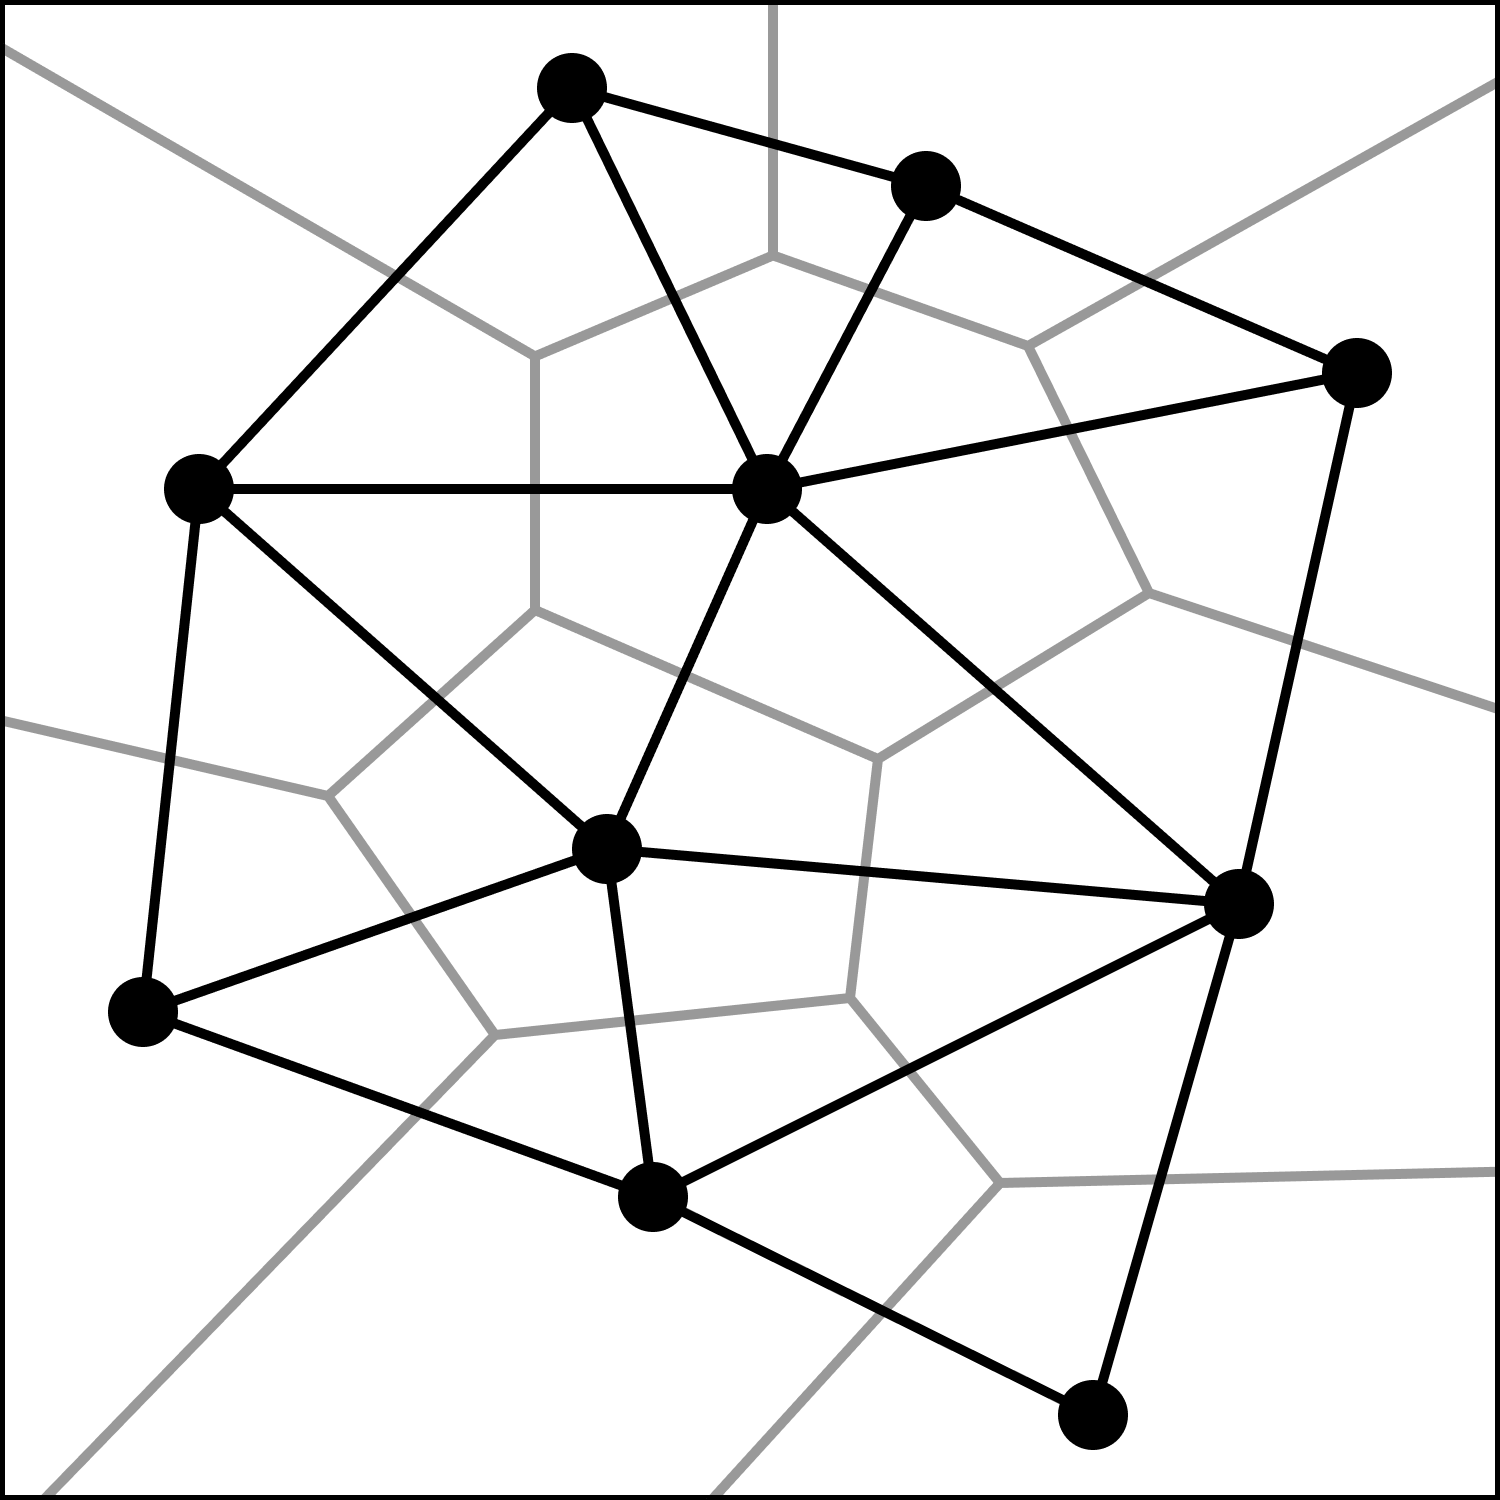
\includegraphics[width=0.48\textwidth]{chapters/algorithms/hnsw/figures/delaunay.png}
    \caption{Delaunay triangulation constructed on top of the Voronoi diagram, connecting points whose Voronoi regions share a boundary.}
    \label{fig:hnsw-3}
\end{figure}

\subsubsection{Skip List}

HNSW can alternatively be interpreted as an extension of the probabilistic skip list structure, where the linked lists are replaced by proximity graphs \cite{Malkov-Yashunin-2016}. This perspective highlights the hierarchical organization of elements across multiple layers, similar to how skip lists allow efficient search through multiple levels of linked nodes.

\subsection{Description of HNSW}

The algorithm organizes elements into multiple layers: upper layers contain longer links and fewer elements, while lower layers contain shorter links and more elements. This design enables efficient search by starting from the upper layer (the "zoom-in" phase), greedily moving toward a local minimum, and then descending to lower layers, restarting from the local minimum found in the previous layer (Figure~\ref{fig:hnsw-4} \cite{Malkov-Yashunin-2016}).

Unlike NSW, elements do not need to be shuffled before insertion. Instead, stochasticity is introduced through level randomization, which supports truly incremental indexing even under temporary changes in data distribution \cite{Malkov-Yashunin-2016}.

\begin{figure}[H]
    \centering
    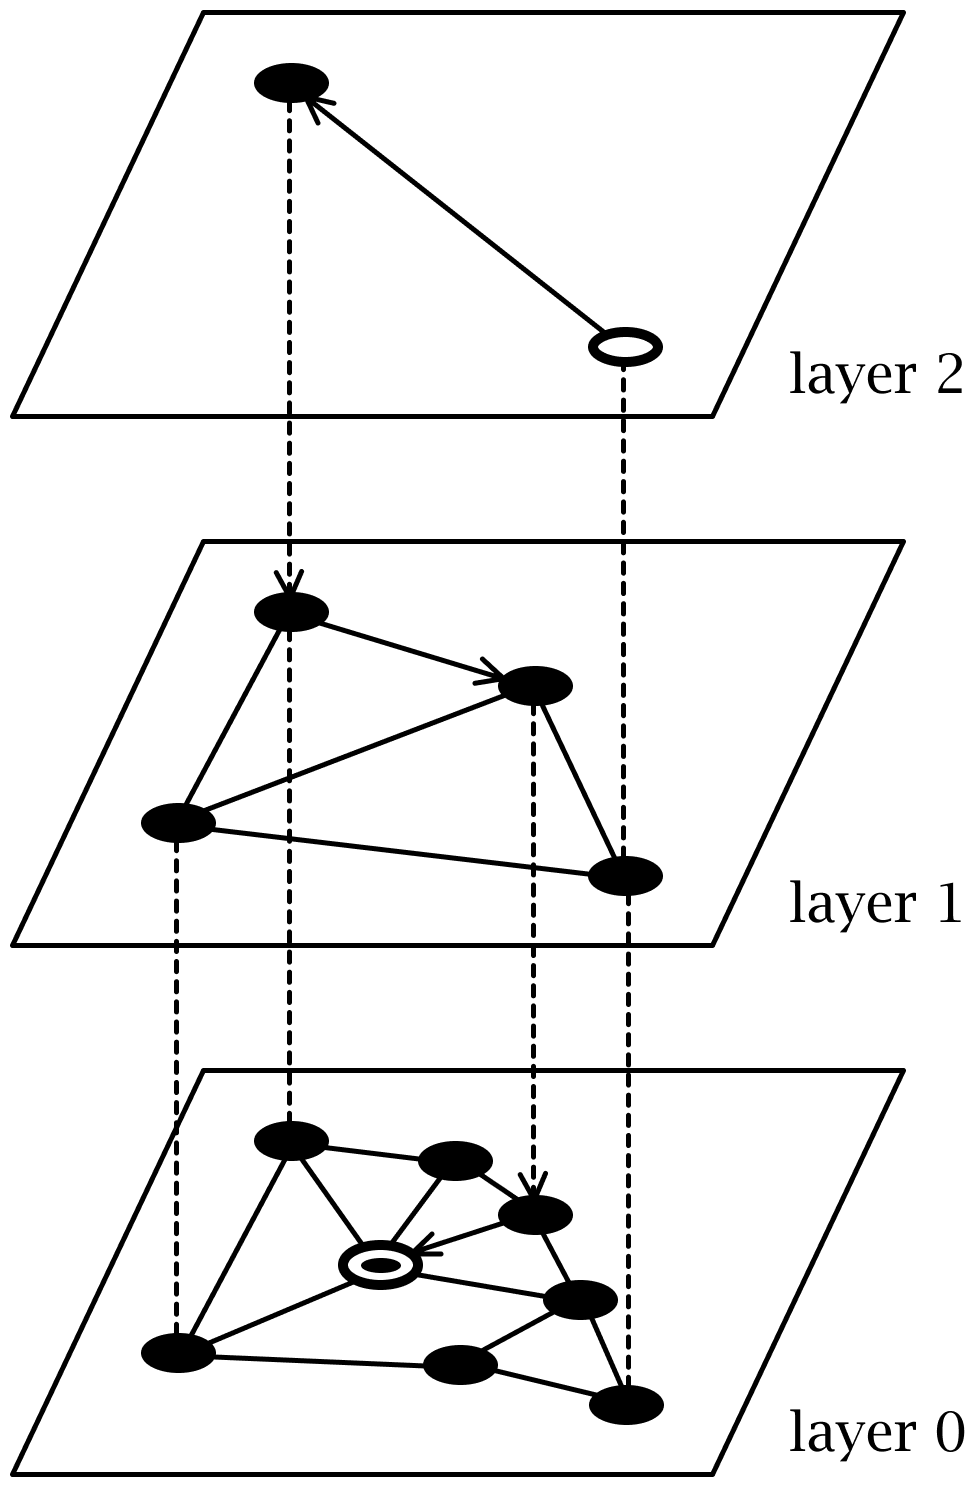
\includegraphics[width=0.4\textwidth]{chapters/algorithms/hnsw/figures/hnsw.png}
    \caption{Graph representation of an HNSW structure. Filled circles represent data points, while the entry point and the query point are indicated as an empty circle and a target circle, respectively. Arrows illustrate the path of the greedy search across layers, starting from the upper layer and descending to lower layers. Upper layers contain longer links and fewer elements, while lower layers contain shorter links and more elements.}
    \label{fig:hnsw-4}
\end{figure}

\paragraph{Element Insertion}

The construction of the HNSW structure is based on consecutive insertions of new elements into the multilayer graph (Algorithm~\ref{alg:hnsw-1}). For each element $q$, a maximum layer $l$ is sampled from a geometric distribution controlled by the parameter $m_L$.

The insertion begins at the top layer $L$, where the algorithm performs a greedy search to find the $ef$ closest neighbors of $q$. The search then proceeds layer by layer down to level $l + 1$, each time using the best candidates from the previous layer as entry points. At layers $l$ down to $0$, the algorithm performs a broader greedy search to identify the $efConstruction$ closest neighbors of $q$, from which up to $M$ are selected to establish bidirectional connections. If the degree of a neighboring element exceeds $M_{\text{max}}$ (or $M_{\text{max0}}$ at the ground layer), its connections are pruned using the same neighbor selection procedure.

Finally, if $q$ is assigned a level higher than the current maximum, it becomes the new entry point of the structure \cite{Malkov-Yashunin-2016}.

\begin{algorithm}[H]
    \caption{INSERT \cite{Malkov-Yashunin-2016}}
    \label{alg:hnsw-1}
    \begin{algorithmic}[1]
        \Require multilayer graph $hnsw$, new element $q$, number of established connections $M$, maximum number of connections per element per layer $M_{\text{max}}$, size of dynamic candidate list $efConstruction$, normalization factor for level generation $m_L$
        \Ensure updated $hnsw$ with element $q$ inserted
        
        \State $W \gets \emptyset$ \Comment{list of currently found nearest elements}
        \State $ep \gets$ get entry point of $hnsw$
        \State $L \gets$ level of $ep$ \Comment{top layer in $hnsw$}
        \State $l \gets \lfloor -\ln(\text{$unif$}(0..1)) \cdot m_L \rfloor$ \Comment{level of new element}
        
        \For{$l_c \gets L \dots l+1$} 
            \State $W \gets \text{SEARCH-LAYER}(q, ep, ef=1, l_c)$
            \State $ep \gets$ get nearest element from $W$ to $q$
        \EndFor
        
        \For{$l_c \gets \min(L,l) \dots 0$} 
            \State $W \gets \text{SEARCH-LAYER}(q, ep, efConstruction, l_c)$
            \State $neighbors \gets \text{SELECT-NEIGHBORS}(q, W, M, l_c)$ \Comment{Algorithm~\ref{alg:hnsw-3} or~\ref{alg:hnsw-4}}
            \State add bidirectional connections from $neighbors$ to $q$ at layer $l_c$
            
            \For{each $e \in neighbors$} \Comment{shrink connections if necessary}
                \State $eConn \gets$ $neighborhood(e)$ at layer $l_c$
                \If{$|eConn| > M_{\text{max}}$} \Comment{shrink connections of $e$ (if $l_c = 0$, then $M_{\text{max}} = M_{\text{max0}}$)}
                    \State $eNewConn \gets \text{SELECT-NEIGHBORS}(e, eConn, M_{\text{max}}, l_c)$ \Comment{Algorithm~\ref{alg:hnsw-3} or~\ref{alg:hnsw-4}}
                    \State set $neighborhood(e)$ at layer $l_c$ to $eNewConn$
                \EndIf
            \EndFor
            
            \State $ep \gets W$
        \EndFor
        
        \If{$l > L$}
            \State set entry point of $hnsw$ to $q$
        \EndIf
    \end{algorithmic}
\end{algorithm}

\paragraph{ANN Layer Search}

To obtain the approximate $ef$ nearest neighbors of a query element $q$ within a given layer $l_c$, the algorithm (Algorithm~\ref{alg:hnsw-2}) maintains a list $W$ of up to $ef$ closest found elements, initialized with the entry points. At each step, the closest non-evaluated element from the candidate set $C$ is selected, and its neighbors are examined. If a neighbor is closer to $q$ than the furthest element currently in $W$, or if $W$ contains fewer than $ef$ elements, it is added to both $C$ and $W$. The process continues until all elements in $C$ have been evaluated.

A key stopping condition is that once the closest candidate in $C$ is further from $q$ than the most distant element in $W$, the search terminates, as no remaining candidates can improve the result. This mechanism prevents unnecessary distance evaluations and avoids bloating of the search structures \cite{Malkov-Yashunin-2016}.

\begin{algorithm}[H]
    \caption{SEARCH-LAYER \cite{Malkov-Yashunin-2016}}
    \label{alg:hnsw-2}
    \begin{algorithmic}[1]
        \Require query element $q$, entry points $ep$, number of nearest neighbors $ef$, layer number $l_c$
        \Ensure $ef$ nearest neighbors to $q$
        
        \State $v \gets ep$ \Comment{set of visited elements}
        \State $C \gets ep$ \Comment{set of candidates}
        \State $W \gets ep$ \Comment{dynamic list of found nearest neighbors}
        
        \While{$|C| > 0$}
            \State $c \gets$ extract nearest element from $C$ to $q$
            \State $f \gets$ get furthest neighbor from $W$ to $q$
            \If{$distance(c, q) > distance(f, q)$}
                \State \textbf{break} \Comment{all elements in $W$ evaluated}
            \EndIf
            
            \For{each $e \in$ $neighborhood(c)$ at layer $l_c$} \Comment{update $C$ and $W$}
                \If{$e \notin v$}
                    \State $v \gets v \cup \{e\}$
                    \State $f \gets$ get furthest neighbor from $W$ to $q$
                    \If{$distance(e, q) < distance(f, q)$ \textbf{or} $|W| < ef$}
                        \State $C \gets C \cup \{e\}$
                        \State $W \gets W \cup \{e\}$
                        \If{$|W| > ef$}
                            \State remove furthest neighbor from $W$ to $q$
                        \EndIf
                    \EndIf
                \EndIf
            \EndFor
        \EndWhile
        
        \State \Return $W$
    \end{algorithmic}
\end{algorithm}

\paragraph{Simple Neighbor Selection}

A straightforward approach for selecting connections in the proximity graph is to simply select the closest elements to the base element from the candidate set (Algorithm~\ref{alg:hnsw-3}). This strategy does not account for the mutual distances between candidates, but only their distances to the base element, which may lead to redundant connections in highly clustered regions of the space \cite{Malkov-Yashunin-2016}.

\begin{algorithm}[H]
    \caption{SELECT-NEIGHBORS-SIMPLE \cite{Malkov-Yashunin-2016}}
    \label{alg:hnsw-3}
    \begin{algorithmic}[1]
        \Require base element $q$, candidate elements $C$, number of neighbors to return $M$
        \Ensure $M$ nearest elements to $q$
        
        \State \Return $M$ nearest elements from $C$ to $q$
    \end{algorithmic}
\end{algorithm}

\paragraph{Heuristic Neighbor Selection}

To address the limitations of the simple strategy, a heuristic procedure is employed for selecting neighbors (Algorithm~\ref{alg:hnsw-4}). The heuristic processes the candidates in order of increasing distance to the base element and establishes a connection to a candidate only if its distance to the base element is smaller than its distance to any of the already selected neighbors. In this way, the algorithm promotes diversity of connections by preventing redundant edges in similar directions.
\newpage
Two optional parameters further refine this method. The first, \textit{extendCandidates}, allows the candidate set to be expanded by including neighbors of the initial candidates; although disabled by default, this option is beneficial in extremely clustered data. The second, \textit{keepPrunedConnections}, enables adding back some of the discarded candidates in order to maintain a fixed number of connections per element \cite{Malkov-Yashunin-2016}.

\begin{algorithm}[H]
    \caption{SELECT-NEIGHBORS-HEURISTIC \cite{Malkov-Yashunin-2016}}
    \label{alg:hnsw-4}
    \begin{algorithmic}[1]
        \Require base element $q$, candidate elements $C$, number of neighbors to return $M$, layer number $l_c$, flag indicating whether or not to extend candidate list $extendCandidates$, flag indicating whether or not to add discarded elements $keepPrunedConnections$
        \Ensure $M$ elements selected by the heuristic

        \State $R \gets \emptyset$
        \State $W \gets C$ \Comment{queue for candidates}

        \If{$extendCandidates$} \Comment{extend candidates by their neighbors}
            \For{each $e \in C$}
                \For{each $e_{adj} \in$ $neighborhood(e)$ at layer $l_c$}
                    \If{$e_{adj} \notin W$}
                        \State $W \gets W \cup \{e_{adj}\}$
                    \EndIf
                \EndFor
            \EndFor
        \EndIf

        \State $W_d \gets \emptyset$ \Comment{queue for discarded candidates}

        \While{$|W| > 0$ \textbf{and} $|R| < M$}
            \State $e \gets$ extract nearest element from $W$ to $q$
            \If{$e$ is closer to $q$ compared to any element from $R$}
                \State $R \gets R \cup \{e\}$
            \Else
                \State $W_d \gets W_d \cup \{e\}$
            \EndIf
        \EndWhile

        \If{$keepPrunedConnections$} \Comment{add some of discarded connections from $W_d$}
            \While{$|W_d| > 0$ \textbf{and} $|R| < M$}
                \State $R \gets R \cup \{$extract nearest element from $W_d$ to $q\}$
            \EndWhile
        \EndIf

        \State \Return $R$
    \end{algorithmic}
\end{algorithm}

\paragraph{$k$-ANN Search}

The retrieval of the $k$ approximate nearest neighbors of a query element $q$ in the HNSW structure (Algorithm~\ref{alg:hnsw-5}) follows a process analogous to inserting a zero-level element. The key distinction is that the closest neighbors at the ground layer are returned as the search result rather than being used to form new connections.

Starting from the top layer $L$, the algorithm traverses down through the layers in a greedy manner. At each layer, the search begins from the element closest to the query found in the previous layer and uses $ef = 1$ to quickly move toward the query. Upon reaching the ground layer ($l_c = 0$), a broader greedy search is conducted with the parameter $ef$ to identify the closest elements, from which the $k$ nearest neighbors are returned \cite{Malkov-Yashunin-2016}.

\begin{algorithm}[H]
    \caption{K-NN-SEARCH \cite{Malkov-Yashunin-2016}}
    \label{alg:hnsw-5}
    \begin{algorithmic}[1]
        \Require multilayer graph $hnsw$, query element $q$, number of nearest neighbors $k$, size of dynamic candidate list $ef$
        \Ensure $k$ nearest neighbors to $q$
        
        \State $W \gets \emptyset$ \Comment{set of current nearest elements}
        \State $ep \gets$ get entry point of $hnsw$
        \State $L \gets$ level of $ep$ \Comment{top layer in $hnsw$}
        
        \For{$l_c \gets L \dots 1$}
            \State $W \gets \text{SEARCH-LAYER}(q, ep, ef=1, l_c)$
            \State $ep \gets$ get nearest element from $W$ to $q$
        \EndFor
        
        \State $W \gets \text{SEARCH-LAYER}(q, ep, ef, l_c=0)$
        \State \Return $k$ nearest elements from $W$ to $q$
        
    \end{algorithmic}
\end{algorithm}

\subsection{Analysis of HNSW}

\subsubsection{Construction Parameters}

The main construction parameters of HNSW are $m_L$, $M_{\text{max0}}$, $M$, and $efConstruction$. These parameters directly influence the graph structure, search performance, and memory usage. The analysis follows \cite{Malkov-Yashunin-2016}.

\paragraph{$m_L$ Parameter}

The parameter $m_L$ controls the probability of assigning elements to higher layers, thereby affecting the hierarchy depth and the navigability of the graph. Its influence can be summarized as: 

\begin{itemize}
    \item $m_L = 0$ and $M_{\text{max0}} = M$: produces a directed $k$-NN graph with power-law complexity.
    \item $m_L = 0$ and $M_{\text{max0}} = \infty$: produces an NSW graph with polylogarithmic complexity.
    \item $m_L > 0$: produces a controllable hierarchy graph with logarithmic complexity.
\end{itemize}

To achieve optimal performance in the controllable hierarchy, the overlap of neighbors across layers (i.e., the percentage of element neighbors shared between layers) should remain small. Reducing $m_L$ decreases this overlap but increases the average number of hops during greedy search, so an optimal tradeoff exists. A practical choice is
\[
m_L = \frac{1}{\ln(M)},
\]
ensuring on average a single overlapping neighbor between layers.

\paragraph{$M_{\text{max0}}$ Parameter}

The parameter $M_{\text{max0}}$ defines the maximum number of connections per element in the ground layer and has a strong influence on search performance, particularly for high-recall queries. Setting $M_{\text{max0}} = M$ leads to a significant performance penalty at high recall. Simulations in \cite{Malkov-Yashunin-2016} suggest that setting $M_{\text{max0}} = 2 \cdot M$ provides good performance, while increasing it further may result in performance degradation and unnecessary memory usage.

\paragraph{$M$ Parameter}

The parameter $M$ defines the number of neighbors to be selected for each element during insertion. It determines how many bidirectional connections a new element establishes in each layer. A reasonable range for $M$ is 5 to 48. Smaller values generally yield better performance for low-dimensional data or low-recall queries, while larger values are more suitable for high-dimensional data or high-recall searches. Memory usage grows proportionally with $M$, so it should be chosen carefully.

\paragraph{$efConstruction$ Parameter}

The parameter $efConstruction$ defines the size of the candidate list used during the insertion of a new element. A sufficiently large $efConstruction$ ensures that most true nearest neighbors of the element are considered, achieving high recall during index construction. Increasing $efConstruction$ can further improve index quality, but at the cost of longer construction times.

\subsubsection{Complexity}

\paragraph{Search Complexity}

A theoretical analysis of a single search, following \cite{Malkov-Yashunin-2016}, assumes exact Delaunay graphs. Suppose the search has identified the closest element at some layer and then descends to the next one. Since the layers are not correlated with the spatial positions of the data points, there is a fixed probability that the next visited node belongs to the upper layer, given by $p = e^{-m_L}$. However, the search within a layer must terminate before reaching such a node; otherwise, the search on the upper layer would have already stopped at a different element. Consequently, the probability of not reaching the target within $s$ steps is bounded by $e^{-s \cdot m_L}$, and the expected number of steps in a layer is given by the geometric series
\[
S = \frac{1}{1 - e^{-m_L}},
\]
which is independent of $N$. If the average degree of a node in the (exact) Delaunay graph is bounded by a constant $C$, then the expected number of distance evaluations per layer is bounded by a constant $C \cdot S$. Since the expected number of layers in the structure grows as $O(\log N)$ by construction, the overall expected search complexity is
\[
O(\log N).
\]

In practice, the assumption of having an exact Delaunay graph is violated in HNSW due to the use of an approximate neighbor selection heuristic with a fixed number of connections per element. To avoid getting stuck in local minima at the ground layer, the greedy search algorithm employs a backtracking procedure. For low-dimensional data, the dependence of the required $ef$ parameter (which controls the number of hops explored during backtracking) on dataset size saturates as $N$ increases, so the backtracking complexity behaves as an additive term and does not affect the overall $O(\log N)$ search scaling \cite{Malkov-Yashunin-2016}.

\paragraph{Construction Complexity}

The index is built by inserting all elements iteratively \cite{Malkov-Yashunin-2016}. Each insertion consists of a sequence of $k$-ANN searches across the layers, followed by applying a heuristic with fixed cost for a given $efConstruction$. The average number of layers an element belongs to is a constant depending only on $m_L$. Therefore, the insertion complexity has the same scaling as the search, and for relatively low-dimensional datasets the overall construction complexity is
\[
O(N \cdot \log N).
\]

\paragraph{Memory Cost}

The memory consumption of HNSW index is primarily determined by the storage of graph connections. Each element has up to $M_{\text{max0}}$ connections in the ground layer and up to $M_{\text{max}}$ connections in all other layers. Therefore, the average memory required per element is 
\[
(M_{\text{max0}} + m_L \cdot M_{\text{max}}) \cdot \text{bytes\_per\_link}.
\]
If the maximum number of elements is limited to approximately four billion, four-byte unsigned integers can be used to store the connections. Typical near-optimal values of $M$ range from 6 to 48, leading to average memory requirements of roughly 60–450 bytes per element, excluding the size of the data itself \cite{Malkov-Yashunin-2016}.

\begin{center}
    \vspace{0.5cm}
    *\hspace{2cm}*\hspace{2cm}*
    \vspace{0.3cm}
\end{center}

Three prominent approaches for approximate nearest neighbor search have been presented: Locality-Sensitive Hashing (LSH), Approximate Nearest Neighbors Oh Yeah (Annoy), and Hierarchical Navigable Small World (HNSW). LSH emphasizes theoretical guarantees and sublinear query time through hash-based partitioning of the data space. Annoy focuses on practical efficiency, using tree-based random projections and supporting memory-friendly, multi-process usage. HNSW combines hierarchical graph structures with scale separation, achieving strong empirical performance and logarithmic search complexity. Together, these methods exemplify three distinct paradigms for approximate nearest neighbor search: hash-based, tree-based, and graph-based.
    \chapter{Vector Databases in Practice}

\section{Systems and Tools}

Vector databases provide specialized infrastructure for managing high-dimensional embeddings, enabling efficient similarity search over large collections of unstructured data. They are optimized for real-time queries, large-scale vector operations, and integrated index management, making them a core component in AI-driven applications.

\paragraph{Vector Databases, Libraries, and Plugins}

Vector search libraries, such as FAISS, are designed to be integrated into the application under development. They provide high-performance ANN search, but scalability becomes an issue as dataset sizes grow.
Traditional relational databases or search systems, such as Elasticsearch, often include built-in vector search plugins. However, these are enhancements on top of existing architectures and are therefore limited in functionality and performance.
Dedicated vector databases, such as Milvus or Weaviate, are purpose-built to deliver scalable, real-time responses and comprehensive APIs for both vector and structured data management.

\subsection{FAISS}

FAISS (Facebook AI Similarity Search) is an open-source\footnote{\url{https://github.com/facebookresearch/faiss}} library for ANN search. Its core is implemented in C++ with no external dependencies and is accompanied by a Python interface, allowing it to be used both in standalone scripts and as a building block for larger systems.

FAISS provides multiple indexing techniques, which may include preprocessing, compression, and non-exhaustive search strategies - specifically, inverted file and graph-based methods, such as HNSW.

At its core, FAISS maintains an index to which database vectors are incrementally added. Queries are submitted as vectors, and the library returns nearest neighbors according to a chosen distance metric, most commonly the Euclidean distance. Variants include returning $k$ nearest neighbors, vectors within a specified radius, batch queries, and execution on CPUs or GPUs.

It is important to note that FAISS does not perform feature extraction, manage concurrency, or provide database services such as sharding, transaction management, or query optimization. Its scope is focused on the algorithmic implementation of ANN search \cite{faiss-2024, faiss-2019}.

\subsection{Milvus}

Milvus is an open-source\footnote{\url{https://github.com/milvus-io/milvus}} vector database. Written in Go and C++, Milvus leverages CPU and GPU acceleration to enhance vector search performance. Kubernetes-native architecture allows horizontal scaling, real-time streaming updates, and deployment in both multi-node clusters and standalone mode.

It stores vectors alongside scalar metadata and enables efficient $k$-NN queries, hybrid search, and metadata filtering. The system supports multiple vector index types, including HNSW, IVF, FLAT, SCANN, and DiskANN, with quantization-based variations.

Milvus also supports sparse vectors for full-text search and hybrid retrieval, combining dense and sparse embeddings within the same collection. Data security is enforced through mandatory authentication, TLS encryption, and role-based access control.

The Milvus ecosystem integrates with various AI development frameworks and provides utilities for embedding transformation, search reranking, administration, monitoring, and data pipeline integration \cite{milvus-2021, milvus-2022}.

\subsection{Weaviate}

Weaviate is an open-source\footnote{\url{https://github.com/weaviate/weaviate}}, cloud-native vector database that stores both objects and vectors, enabling semantic search at scale. It combines vector similarity search with keyword filtering, retrieval-augmented generation (RAG), and reranking in a single query interface, supporting applications such as RAG systems, semantic and image search, recommendation engines, chatbots, and content classification.

Weaviate allows vectors to be either automatically generated at import using integrated models (e.g., OpenAI, Cohere, HuggingFace) or directly imported as pre-computed embeddings. Its production-ready features include multi-tenancy, replication, fine-grained role-based access control (RBAC), and horizontal scaling.

The system supports advanced hybrid search by combining semantic, keyword (BM25), and image search, and integrates generative RAG and reranking capabilities. Performance optimizations, such as vector compression and multi-vector encoding, reduce memory usage while maintaining fast, millisecond-scale retrieval over billions of vectors \cite{weaviate-weaviate}.
\section{Practical Applications}

This section demonstrates the practical applications of vector databases through experiments with FAISS, Milvus, and Weaviate. The aim is to illustrate how embeddings can be stored, indexed, and queried.

Experiments were conducted using Google Colab to provide a consistent and accessible execution environment. FAISS, being a standalone library, was integrated directly into the Colab notebook without additional setup. For Milvus and Weaviate, cloud-based sandbox environments were employed. Each service required the creation of a cluster, followed by retrieval of the connection parameters necessary to interact with the respective database. Once the environments were established, all subsequent operations, including collection creation, embeddings insertion, indexing, and nearest neighbors search, were executed through the code examples presented in this section.

\subsection{Image Search}

Image search involves retrieving visually or semantically similar images given a query image. Traditional approaches, relying on exact pixel comparisons or handcrafted features, often fail to capture higher-level semantic content and do not scale efficiently to large datasets. Representing images as high-dimensional embeddings allows the use of nearest neighbor techniques to measure similarity in a feature space that encodes semantic relationships. Vector databases facilitate efficient storage, indexing, and retrieval of these embeddings, enabling nearest neighbor search even over large-scale datasets. This makes the approach a practical and scalable solution for content-based image retrieval tasks.

\paragraph{Dataset and Embeddings}

Demonstrations were conducted on a subset of the CIFAR-10 dataset, consisting of 60,000 color images of size $32 \times 32$ pixels, evenly distributed across ten object classes. Each image in the subset is labeled according to its class (\texttt{labels}). Feature embeddings were extracted using a pretrained ResNet-18 model, yielding high-dimensional representations suitable for nearest neighbor search (\texttt{embeddings}). Detailed dataset preparation and embeddings extraction steps are provided in Appendix~\ref{app:dataset-and-embeddings}.

\paragraph{Demonstrations}

The examples provided below illustrate the use of vector management systems and tools for nearest neighbor search on image embeddings. The demonstration uses pre-extracted variables including the embedding dimension (\texttt{d}), the query vector (\texttt{query\_vector}, corresponding to the first image in the subset), and the number of nearest neighbors (\texttt{k}, set to 10). The label of the query image is 6, which occurs in 207 images within the subset. Definitions of these variables are provided in Appendix~\ref{app:variables-extraction}. Below each code example, the output shows the $k$ returned IDs and their corresponding labels.

\subsubsection{FAISS HNSW}

The first example demonstrates the use of the FAISS library, employing the HNSW algorithm for approximate nearest neighbor search. The code performs $k$-NN search using pre-extracted embeddings, as shown in Listing~\ref{lst:faiss-hnsw}.

\begin{lstlisting}[
    caption={$k$-NN search using FAISS HNSW approach.},
    label={lst:faiss-hnsw}
]
import numpy as np
import faiss

index_hnsw = faiss.IndexHNSWFlat(d, 32)  # M=32
index_hnsw.hnsw.efConstruction = 40
index_hnsw.add(embeddings)

index_hnsw.hnsw.efSearch = 50
distances_hnsw, indices_hnsw = index_hnsw.search(query_vector.reshape(1, -1), k)

print("Top-k indices:", indices_hnsw[0].tolist())
print("Top-k labels:", labels[indices_hnsw[0]].tolist())
\end{lstlisting}
{\small
\begin{verbatim}
Top-k indices: [0, 1002, 1484, 228, 1393, 314, 1635, 1596, 27, 1202]
Top-k labels: [6, 3, 6, 6, 6, 3, 6, 6, 5, 3]
\end{verbatim}
}

\subsubsection{Milvus HNSW}

The second example demonstrates the use of Milvus, a cloud-based vector database. Connection setup details are provided in Appendix~\ref{app:milvus-connection}. The code performs $k$-NN search using pre-extracted embeddings, as shown in Listing~\ref{lst:milvus-hnsw}.

\begin{lstlisting}[
    caption={$k$-NN search using Milvus HNSW approach.},
    label={lst:milvus-hnsw}
]
import numpy as np
from pymilvus import FieldSchema, DataType, CollectionSchema, Collection, list_collections

collection_name = "CIFAR10"

# Drop the collection if it already exists to ensure a clean start
if collection_name in list_collections():
    Collection(collection_name).drop()

# Define and create the collection schema
# 'index' serves as the primary key, 'embedding' stores the image vectors
collection = Collection(
    collection_name,
    CollectionSchema([
        FieldSchema(name="index", dtype=DataType.INT64, is_primary=True),
        FieldSchema(name="embedding", dtype=DataType.FLOAT_VECTOR, dim=d)
    ])
)

# Insert embeddings with their indices and flush to persist data
collection.insert([np.arange(len(embeddings)), embeddings])
collection.flush()

# Create an HNSW index on the embedding field
index_params = {"index_type": "HNSW", "metric_type": "L2", "params": {"M": 32, "efConstruction": 40}}
collection.create_index(field_name="embedding", index_params=index_params)

# Load the collection into memory to enable search
collection.load()

# Define search parameters and perform top-k nearest neighbor search
search_params = {"metric_type": "L2", "params": {"ef": 50}}
results = collection.search([query_vector], "embedding", search_params, limit=k)

top_ids = [res.index for res in results[0]]
print("Top-k ids:", top_ids)
print("Top-k labels:", labels[top_ids].tolist())
\end{lstlisting}
{\small
\begin{verbatim}
Top-k ids: [0, 1002, 1484, 228, 1393, 314, 1635, 1596, 27, 865]
Top-k labels: [6, 3, 6, 6, 6, 3, 6, 6, 5, 3]
\end{verbatim}
}

\subsubsection{Weaviate HNSW}

The third example demonstrates the use of Weaviate, a cloud-based vector database. Connection setup details are provided in Appendix~\ref{app:weaviate-connection}. The code performs $k$-NN search using pre-extracted embeddings, as shown in Listing~\ref{lst:weaviate-hnsw}.

\begin{lstlisting}[
    caption={$k$-NN search using Weaviate HNSW approach.},
    label={lst:weaviate-hnsw}
]
import weaviate.classes as wvc

collection_name = "CIFAR10"

# Drop the collection if it already exists to ensure a clean start
if collection_name in client.collections.list_all():
    client.collections.delete(collection_name)

# Create a new collection with a single INT property 'index'
# vector_config=self_provided() indicates that embeddings are precomputed
collection = client.collections.create(
    name=collection_name,
    properties=[wvc.config.Property(name="index", data_type=wvc.config.DataType.INT)],
    vector_config=wvc.config.Configure.Vectors.self_provided()
)

# Insert embeddings with their unique indices
collection.data.insert_many([
    wvc.data.DataObject(properties={"index": i}, vector=e)
    for i, e in enumerate(embeddings)
])

# Perform top-k nearest neighbor search
response = collection.query.near_vector(near_vector=query_vector, limit=k)

top_ids = [res.properties["index"] for res in response.objects]
print("Top-k ids:", top_ids)
print("Top-k labels:", labels[top_ids].tolist())
\end{lstlisting}
{\small
\begin{verbatim}
Top-k ids: [0, 1819, 1635, 314, 1002, 1628, 265, 1246, 1646, 1393]
Top-k labels: [6, 6, 6, 3, 3, 6, 9, 6, 6, 6]
\end{verbatim}
}

\newpage

\subsection{Recommendation Systems}

Recommendation systems aim to predict user preferences and suggest relevant items, such as products, movies, or songs. High-dimensional embeddings can represent both users and items in a shared feature space, capturing latent characteristics and similarities. Vector databases enable efficient nearest neighbor search to identify items most similar to a given user profile or query item, supporting real-time personalized recommendations even for very large catalogs. Approximate nearest neighbor search allows scaling to millions of items without sacrificing responsiveness.

\subsection{Document Retrieval and Analysis}

Document retrieval and analysis involve searching, clustering, and organizing large collections of unstructured text data. Embeddings derived from language models capture semantic relationships between documents beyond keyword matching. Storing these embeddings in vector databases allows for fast similarity search, enabling tasks such as semantic search, document clustering, and question-answering over large corpora. This approach provides both efficiency and scalability, crucial for handling modern text-intensive applications.

\begin{center}
    \vspace{0.5cm}
    *\hspace{2cm}*\hspace{2cm}*
    \vspace{0.3cm}
\end{center}

Vector databases provide purpose-built infrastructure for storing and querying embeddings at scale, enabling a wide range of AI applications. Libraries like FAISS offer algorithmic building blocks, while dedicated databases such as Milvus and Weaviate provide fully-managed solutions. Together, these technologies illustrate the spectrum of tools available for managing unstructured data in practical scenarios.

The Google Colab notebook\footnote{\url{https://colab.research.google.com/drive/1JHNvJkmdoVusyAvnL5KEk_dYkhFJgKAa?usp=sharing}} containing the demonstrations presented in this chapter is publicly available for viewing.
    
    \chapter*{Conclusion}

This thesis has examined the theoretical foundations and practical applications of vector databases, with a particular focus on approximate nearest neighbor (ANN) search in high-dimensional spaces. Through detailed analysis of ANN paradigms, including hash-based methods (LSH), tree-based methods (Annoy), and graph-based methods (HNSW), the study clarified their operational principles, advantages, and limitations, providing insights that complement existing literature.

The practical investigation highlighted contemporary vector management systems such as FAISS, Milvus, and Weaviate. By generating embeddings from a representative dataset, constructing indices, and executing similarity searches, the thesis demonstrated how these systems can be effectively leveraged in real-world scenarios. This hands-on component validated theoretical concepts and provided a clear workflow for implementing similarity search in high-dimensional spaces.

\section*{Achieved Objectives of the Thesis}

The primary objectives set at the outset have been successfully met:

\begin{itemize}
    \item Established a comprehensive theoretical foundation, covering vector representations, similarity measures, and nearest neighbor search principles.
    \item Analyzed approximate nearest neighbor algorithms, including hash-based (LSH), tree-based (Annoy), and graph-based (HNSW) methods, highlighting their characteristics, advantages, and limitations.
    \item Demonstrated the practical application of vector databases through FAISS, Milvus, and Weaviate, including embeddings storage, index construction, and similarity-based querying, with experiments that bridged theory and practice on real datasets.
\end{itemize}

\section*{Future Directions}

Building on the work presented in this thesis, future research could focus on enhancing performance and scalability through techniques such as multithreading, CPU-level optimizations, and low-level programming, which were beyond the scope of this study. Other promising directions include the development of hybrid ANN algorithms, large-scale distributed vector database architectures, and tighter integration with AI pipelines to improve retrieval efficiency and versatility.
    
    \begin{appendices}
        \chapter{Code Listings}

\section{Dataset and Embeddings}
\label{app:dataset-and-embeddings}
\begin{lstlisting}[
    caption={Dataset preparation and embeddings extraction.},
    label={lst:dataset}
]
import numpy as np
import torch, torchvision
import torchvision.transforms as transforms
from torchvision.models import resnet18, ResNet18_Weights

# Select device: GPU if available, otherwise CPU
device = torch.device("cuda" if torch.cuda.is_available() else "cpu")

# Define image transformations for ResNet input
transform = transforms.Compose([
    transforms.Resize((224, 224)),   # ResNet standard input size
    transforms.ToTensor(),
    transforms.Normalize(
        mean=[0.485, 0.456, 0.406],  # ImageNet mean
        std=[0.229, 0.224, 0.225]    # ImageNet std
    )
])

# Load CIFAR-10 dataset (subset for demonstration)
dataset = torchvision.datasets.CIFAR10(
    root='./data',
    train=True,
    download=True,
    transform=transform
)

subset_size = 2000
subset_indices = list(range(subset_size))
subset = torch.utils.data.Subset(dataset, subset_indices)
loader = torch.utils.data.DataLoader(subset, batch_size=64, shuffle=False)

# Initialize pretrained ResNet18 model
model = resnet18(weights=ResNet18_Weights.DEFAULT)
model.fc = torch.nn.Identity()  # Remove classification layer to get embeddings
model = model.to(device)
model.eval()

# Compute embeddings for each image in the subset
embeddings = []
labels = []

with torch.no_grad():
    for images, lbls in loader:
        images = images.to(device)
        emb = model(images)  # Extract feature vectors
        embeddings.append(emb.cpu().numpy())
        labels.extend(lbls.numpy())

# Convert lists to NumPy arrays for downstream usage
embeddings = np.vstack(embeddings)
labels = np.array(labels)

print("Embeddings shape:", embeddings.shape)
print("Labels shape:", labels.shape)
\end{lstlisting}

\section{Variables Extraction}
\label{app:variables-extraction}
\begin{lstlisting}[
    caption={Extraction of variables used in demonstration examples.},
    label={lst:vars}
]
# Embedding dimension
d = embeddings.shape[1]

# Query vector: first sample in dataset
query_vector = embeddings[0]

# Number of nearest neighbors to retrieve
k = 10

print(f"Query label: {labels[0]}")
print(f"Number of samples with label {labels[0]}: {np.sum(labels == labels[0])}")
\end{lstlisting}

\newpage

\section{Milvus Connection}
\label{app:milvus-connection}
\begin{lstlisting}[
    caption={Connection to Milvus cluster from Google Colab.},
    label={lst:milvus-connection}
]
from pymilvus import connections

connections.connect(
    alias="default",
    uri="YOUR_URI",
    token="YOUR_TOKEN"
)
\end{lstlisting}

\section{Weaviate Connection}
\label{app:weaviate-connection}
\begin{lstlisting}[
    caption={Connection to Weaviate cluster from Google Colab.},
    label={lst:weaviate-connection}
]
import weaviate
from weaviate.classes.init import Auth

client = weaviate.connect_to_weaviate_cloud(
    cluster_url="YOUR_CLUSTER_URL",
    auth_credentials=Auth.api_key("YOUR_API_KEY")
)
\end{lstlisting}
    \end{appendices}
    
    \backmatter
    
    \addcontentsline{toc}{chapter}{Bibliography}
    \bibliographystyle{IEEEtran} 
    \bibliography{references}
    
    %\addcontentsline{toc}{chapter}{Index}
    %\printindex
\end{document}